\documentclass[slovak,master]{diploma}
\usepackage{subfig}
\usepackage{makecell}
\usepackage[symbol]{footmisc}
\usepackage{wrapfig}
\usepackage{listings}
\usepackage[autostyle=true,czech=quotes]{csquotes} % korektni sazba uvozovek, podpora pro balik biblatex
\usepackage[backend=biber, style=iso-numeric, alldates=iso]{biblatex} % bibliografie
\renewcommand{\thefootnote}{\arabic{footnote}}

\ThesisAuthor{Bc. Matúš Ozaniak}

\ThesisSupervisor{Mgr. Ing. Michal Krumnikl, Ph.D.}

\CzechThesisTitle{Protokol pre komunikáciu medzi uzlami siete LoRa}

\EnglishThesisTitle{LoRa-Based Protocol for Peer-to-Peer Long-Range Communication}

\SubmissionYear{2022}

\ThesisAssignmentFileName{ThesisSpecification_OZA0016.pdf}

\Acknowledgement{
Rád by som sa poďakoval svojmu vedúcemu diplomovej práce pánovi Mgr. Ing. Michalovi Krumniklovi, Ph.D. za 
odborné vedenie, konzultácie a podnety k diplomovej práci.
}

\CzechAbstract{
Technologie LoRa je v současné době jednou z nejslibnějších pro internet věcí a získává si velkou pozornost.
V současných aplikacích však existují omezení způsobená použitou specifikací LoRaWAN, která používá hvězdicovou topologií.
Sítě založené na LoRaWAN mají obvykle omezenou škálovatelnost kvůli použití strategie centralizované správy.
Nedávný pokrok v různých konstrukcích sítí LoRa mesh může představovat potenciální řešení těchto omezení.
V této práci se zabýváme návrhem a implementací protokolu, který umožňuje komunikaci mezi uzly sítě LoRa s využitím topologie mesh.
Protokol vyvinutý v této práci se zaměřuje na komunikaci v reálném čase prostřednictvím technologie LoRa a jako ukázka byla vyvinuta aplikace
určená především pro chatovou komunikaci mezi uživateli v síti mesh. Součástí sítě však mohou být i senzorové uzly, které do sítě odesílají data ze senzorů.
}

\CzechKeywords{LoRa; Mesh; Raspberry Pi; Komunikační protokol; IoT; Diplomová práce}

\EnglishAbstract{
LoRa technology is currently one of the most promising for IoT and is gaining a lot of attention. 
However, there are limitations in current applications due to the LoRaWAN specification used, which uses a star topology. 
LoRaWAN-based networks typically have limited scalability due to the use of a centralized management strategy. 
Recent advances in various LoRa mesh network designs may present a potential solution to these limitations.
In this work, we address the design and implementation of a protocol that enables communication between LoRa network nodes using a mesh topology. 
The protocol developed in this thesis focuses on real time communication through LoRa technology and as a demonstration an application has been developed 
primarily intended for chat communication between users in a mesh network. However, sensor nodes can also be part of the network, sending data from the sensors to the network.
}

\EnglishKeywords{LoRa; Mesh; Raspberry Pi; Communication protocol; IoT; Master's thesis}

\AddAcronym{IoT}{Internet of Things - Internet vecí}
\AddAcronym{SF}{Spreading factor - rozprestierací faktor}
\AddAcronym{BW}{Bandwidth - širka pásma}
\AddAcronym{DR}{Data rate - rýchlosť prenosu}
\AddAcronym{CR}{Coding rate - kódovací pomer}
\AddAcronym{TDMA}{Time Division Multiple Access - Metóda zdielaného prístupu k prenosovemu médiu, ktorá rozdeluje prístup na časové sloty}
\AddAcronym{TTL}{Time To Live - Čas životnosti paketu}
\AddAcronym{SNR}{Signal to Noise ratio - Pomer signálu k šumu}
\AddAcronym{RSSI}{Received Signal Strength Indicator - Miera sily signálu}
\AddAcronym{API}{Aplication Programming Interface - Rozhranie aplikácie}
\AddAcronym{LPWAN}{Low Power Wide Area Network}
\AddAcronym{FEC}{Forward Error Correction}
\AddAcronym{LoRa}{Long Range}
\AddAcronym{LoRaWAN}{Long Range Wide Area Network}
\AddAcronym{SPI}{Serial Peripheral Interface}


\addbibresource{biblatex.bib}

\begin{document}

\MakeTitlePages

\listoffigures
\clearpage

\listoftables
\clearpage

\chapter{Úvod}
V dnešnej dobe sa čoraz viac stretávame s pojmom IoT alebo internet vecí. Jedna sa o lokálne siete, zložené z fyzických zariadení, ktoré tvoria uzly siete.
Zariadenia môžu byť jednoduché senzory na monitorovanie nejakej fyzikálnej veličiny, domáce spotrebiče, vozidla, prípadne 
zariadenia, ktoré je možné ovládať na diaľku. Zariadenia tvoria sieť, v ktorej si môžu medzi sebou posielať 
dáta.

K realizácií takejto siete je potrebné mať niečo, čo by zariadenia spájalo a umožňovalo im komunikáciu. Veľmi používanou technológiou
v tejto oblasti je práve technológia LoRa, ktorá umožňuje bezdrôtovú komunikáciu na veľmi veľké vzdialenosti.

Často je využívané riešenie LoRaWAN, ktoré sa skladá z centrálnych uzlov pripojených k internetu a zariadení, ktoré sú pripojené k centrálnym uzlom pomocou LoRa. 
Zariadenia potom komunikujú len s centrálnym uzlom a predávajú mu svoje dáta. Centrálny uzol dáta môže posielať cez internet na nejakú službu kde 
k ním môžu užívatelia pristupovať z internetu.

Pri LoRaWAN je potrebné mať nejaký centrálny uzol a ak chceme nejaké zariadenie pripojiť do siete, musí mať dosah na daný centrálny uzol. 
Takto sme limitovaní existenciou a dosahom centrálnych uzlov, a hviezdicovou topológiou, čož nie je v niektorých prípadoch užitia vhodné. Neustále vznikajú nové 
protokoly, ktoré by tieto problémy riešili, napríklad za použitia mesh topológii \cite{9385408}.

V tejto práci sa venujeme návrhu a vytvoreniu protokolu, ktorý umožňuje komunikáciu medzi zariadeniami v sieti tvorenej pomocou technológie LoRa,
bez nutnej existencie centrálnych uzlov. Nami vytvorený protokol vytvára sieťovú topológiu typu mesh, ktorá ma oproti hviezdicovej topológii, 
využívanej pri LoRaWAN, niekoľko výhod. Su nimi napríklad škálovatelnosť siete, kedy sa môžu zo siete odoberať alebo do nej pridávať nové zariadenia, 
bez nutnosti akejkoľvek konfigurácie na ostatných zariadeniach. Z toho vyplýva aj vyššia mobilita zariadení. Zariadenia sa môžu fyzicky pohybovať a 
pokiaľ sa nachádzajú v dosahu hocijakého iného uzla, majú prístup do siete.

\chapter{LoRa a spôsob prenosu dát}
V dnešnej dobe sa na trhu nachádza veľa rôznych technológií, ktoré umožňujú bezdrôtovú komunikáciu. Niektoré technológie, ako napríklad Bluetooth, sú vhodné pre komunikáciu na malé 
vzdialenosti, napríklad komunikácia medzi mobilným telefónom a smart hodinkami. Zatiaľ čo iné technológie ako napríklad WiFi nám ponúkajú možnosť komunikácie na väčšie vzdialenosti. 
Nie všetky technológie su však vhodné pre použitie v IoT sieťach. V IoT sieťach sa často dbá na predpoklad nízkej spotreby energie. Okrem nízkej spotreby energie je taktiež vhodné 
aby mal bezdrôtový prenos veľký dosah. Z týchto dôvodov sa pri IoT sieťach využívajú takzvané LPWAN siete.
\section {LPWAN}
LPWAN (Low Power Wide Area Network) je kategória sieti s veľkou rozlohou a nízkou spotrebou energie. Tieto siete sa vyznačujú nízkymi obstarávacími 
nákladmi a dlhodobou prevádzkou. Siete sú tvorené jednoduchými a často pomerné lacnými zariadeniami, ktoré vďaka nízkej spotrebe energie dokážu pracovať dlhú dobu bez 
nutnosti stáleho pripojenia do elektrickej siete. Zariadenia bývajú napájane batériami a môžu nepretržite fungovať aj niekoľko rokov. V kombinácií so solárnymi panelmi 
môže byť ich prevádzka ešte predĺžená. 

Tieto siete sú teda vhodné pre aplikácie, kde je potrebná dlhodobá prevádzka bez nutných servisných zásahov.

LPWAN siete majú veľké pokrytie, v niektorých prípadoch to môžu byť až desiatky kilometrov v otvorenom priestranstve. Zväčša využívajú na prenos 
ultrakrátke ( sub-GHz ) frekvenčné pásma, ktoré nevyžadujú na používanie žiadnu rádiovú licenciu.

Medzi tie najznámejšie technológie na realizáciu LPWAN sieti patria napríklad Sigfox \cite{sigfox}, LoRa \cite{lora}, NB-IoT (NarrowBand Internet of Things) a iné.

\section {LoRa}
LoRa je proprietárna technológia na bezdrôtový prenos dát za pomoci rádiových vĺn.
Používa bez-licenčné rádiové pásma, ktoré sú odlišné medzi Európou, Amerikou a Áziou \cite{loraRegionalParameters}, a poskytuje rádiový prenos na veľkú vzdialenosť s nízkou spotrebou energie.
V otvorenom priestranstve môže mať rádiový prenos dosah až 10--15 km \cite{loraDoc}. LoRa má však veľkú limitáciu v podobe nízkej rýchlosti prenosu dát.
Rýchlosti prenosu sa pohybujú medzi 0,3 až 37,5 kbps v závislosti na vybraných parametroch.

Vďaka týmto aspektom je vhodná pre použitie v IoT senzorových sieťach, kde sa často vyskytujú senzory poháňané batériami a je potrebné aby vydržali dlhú dobu 
bez výmeny batérií. Okrem toho senzory väčšinou odosielajú veľmi malý obsah dát a dáta posielajú iba v určitých časových intervaloch (napr. raz za hodinu), 
takže nízka prenosová rýchlosť v tomto prípade nie je až tak veľkou limitáciou.

Na prenos dát v LoRa, je použitá proprietárna frequency hopping chirp spread-spectrum modulácia -- modulácia rozprestreného spektra s preskokom frekvencií, pri ktorej sú prenášané dáta kódovane do symbolov 
a každý vysielaný symbol je prenášaný takzvaným chirp signálom, do ktorého sa daný symbol moduluje.

Chirp signál ma konštantnú amplitúdu ale mení svoju frekvenciu lineárne s časom. 
Frekvencia sa mení v rozmedzí od spodnej hranice frekvenčného pásma, po hornú hranicu frekvenčného pásma.
Po dosiahnutí hraničnej frekvencie sa frekvencia vráti na opačnú hranicu a proces sa opakuje.
Frekvenčné pásmo, v ktorom sa chirp signál prenáša je určené vybranou šírkou pásma.
Graf frekvenčnej charakteristiky a postupné zvyšovanie frekvencie chirp signálu môžme vidieť na Obr. \ref{fig:loraSymbols}.
\begin{figure}
	\centering
	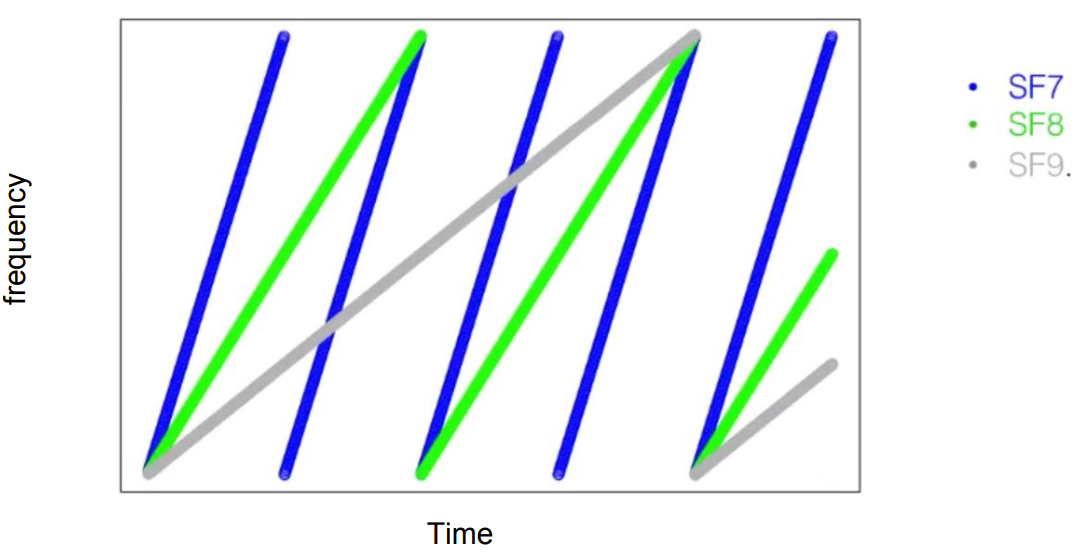
\includegraphics[width=0.7\textwidth]{Figures/spreading factors.png}
	\caption{Chirp signál a porovnanie rozprestieracích faktorov. Prevzaté z \cite{spreadfactorimage}}
	\label{fig:spreadingfactors}
\end{figure}

Existujú dva druhy chirp signálov, sú nimi up-chirp signál a down-chirp signál. Pri up-chirp signále sa prechádza zo spodnej hranice frekvenčného pásma do hornej hranice a pri 
down-chirp zase naopak.

\newpage
Ako rýchlo sa chirp posúva po frekvenčnom pásme - tzn. ako rýchlo chirp signál mení svoju frekvenciu, je určené parametrom rozprestierací faktor -- spreading factor (SF). 
Rozprestierací faktor zároveň vyjadruje, koľko bitov informácie je v každom symbole prenesených. Pri nižšom rozprestieracom faktore sa chirp signál posúva po 
frekvenčnom pásme rýchlejšie (viď Obr. \ref{fig:spreadingfactors}) a tým sa zvyšuje rýchlosť dátového prenosu, 
avšak zhoršuje sa citlivosť, ktorou dokáže prijímač prijať signál a dôsledkom toho je menší použiteľný dosah.

Každý chirp signál je rozdelený na X častí -- tzv. chips. Tieto chips predstavujú skoky vo vysielacej frekvencii signálu. 
Koľko týchto chips jeden chirp obsahuje je závisle od vybraného rozprestieracieho faktoru. 
Jeden chirp je rozdelený na $2^{SF}$ častí alebo chips.

Vysielaný symbol sa potom skladá z cyklicky posunutého chirp signálu, kde posun definuje hodnotu daného symbolu. 
To znamená, že vysielaný chirp nebude začínať na spodnej hranici frekvenčného pásma, ale na určitej frekvencii korešpondujúcej so symbolom, 
ktorý je modulovaný do daného chirp signálu. Viď Obr. \ref{fig:loraSymbols}.

\begin{figure}
	\centering
	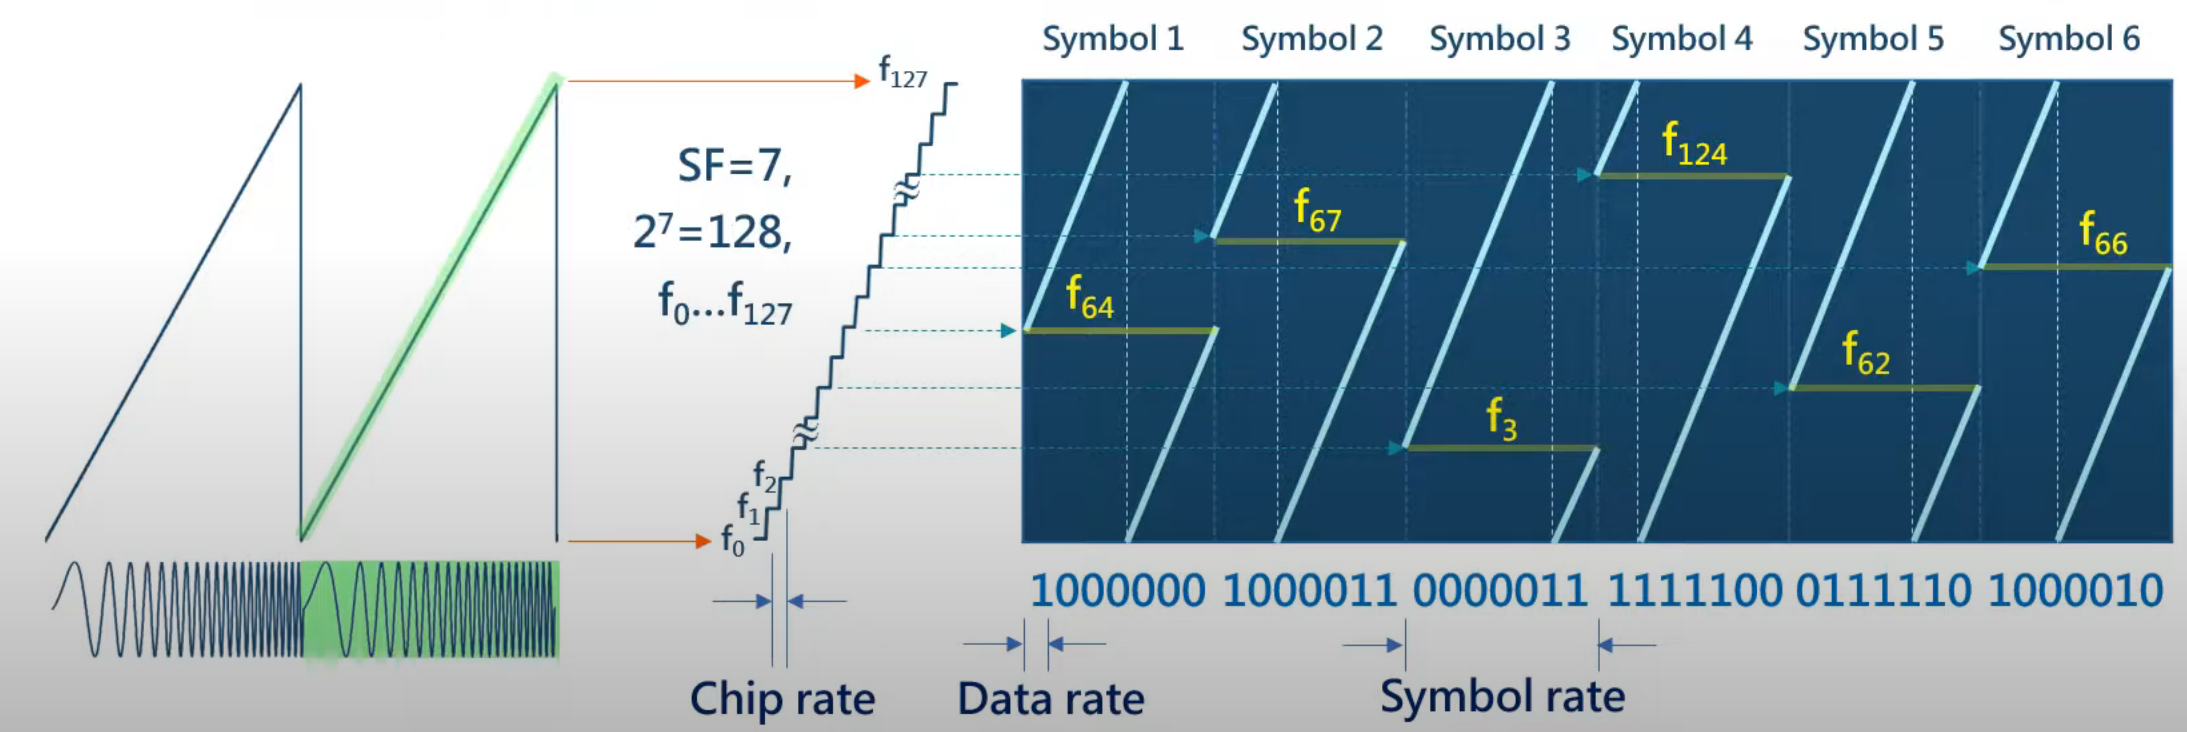
\includegraphics[width=1\textwidth]{Figures/loraSymbols.png}
	\caption{Chirp signály, do ktorých boli modulované symboly. \cite[Prevzaté z video prezentácie výrobcu GW Instek]{loratester}}
	\label{fig:loraSymbols}
\end{figure}

Celý proces vyslania správy cez LoRa sa teda skladá z nasledujúcich krokov:
\begin{enumerate}
  \item Konverzia správy do binárneho kódu
  \item Pridanie korekčných bitov slúžiacich na opravu chýb
  \item Pridanie preambuly a kontrolného súčtu, a poskladanie do LoRa paketu
  \item Modulácia bitov do chirp signálov
  \item Odvysielanie chirp signálov
\end{enumerate}
Ukážku môžme vidieť na Obr. \ref{fig:loraModulation}.

\begin{figure}
	\centering
	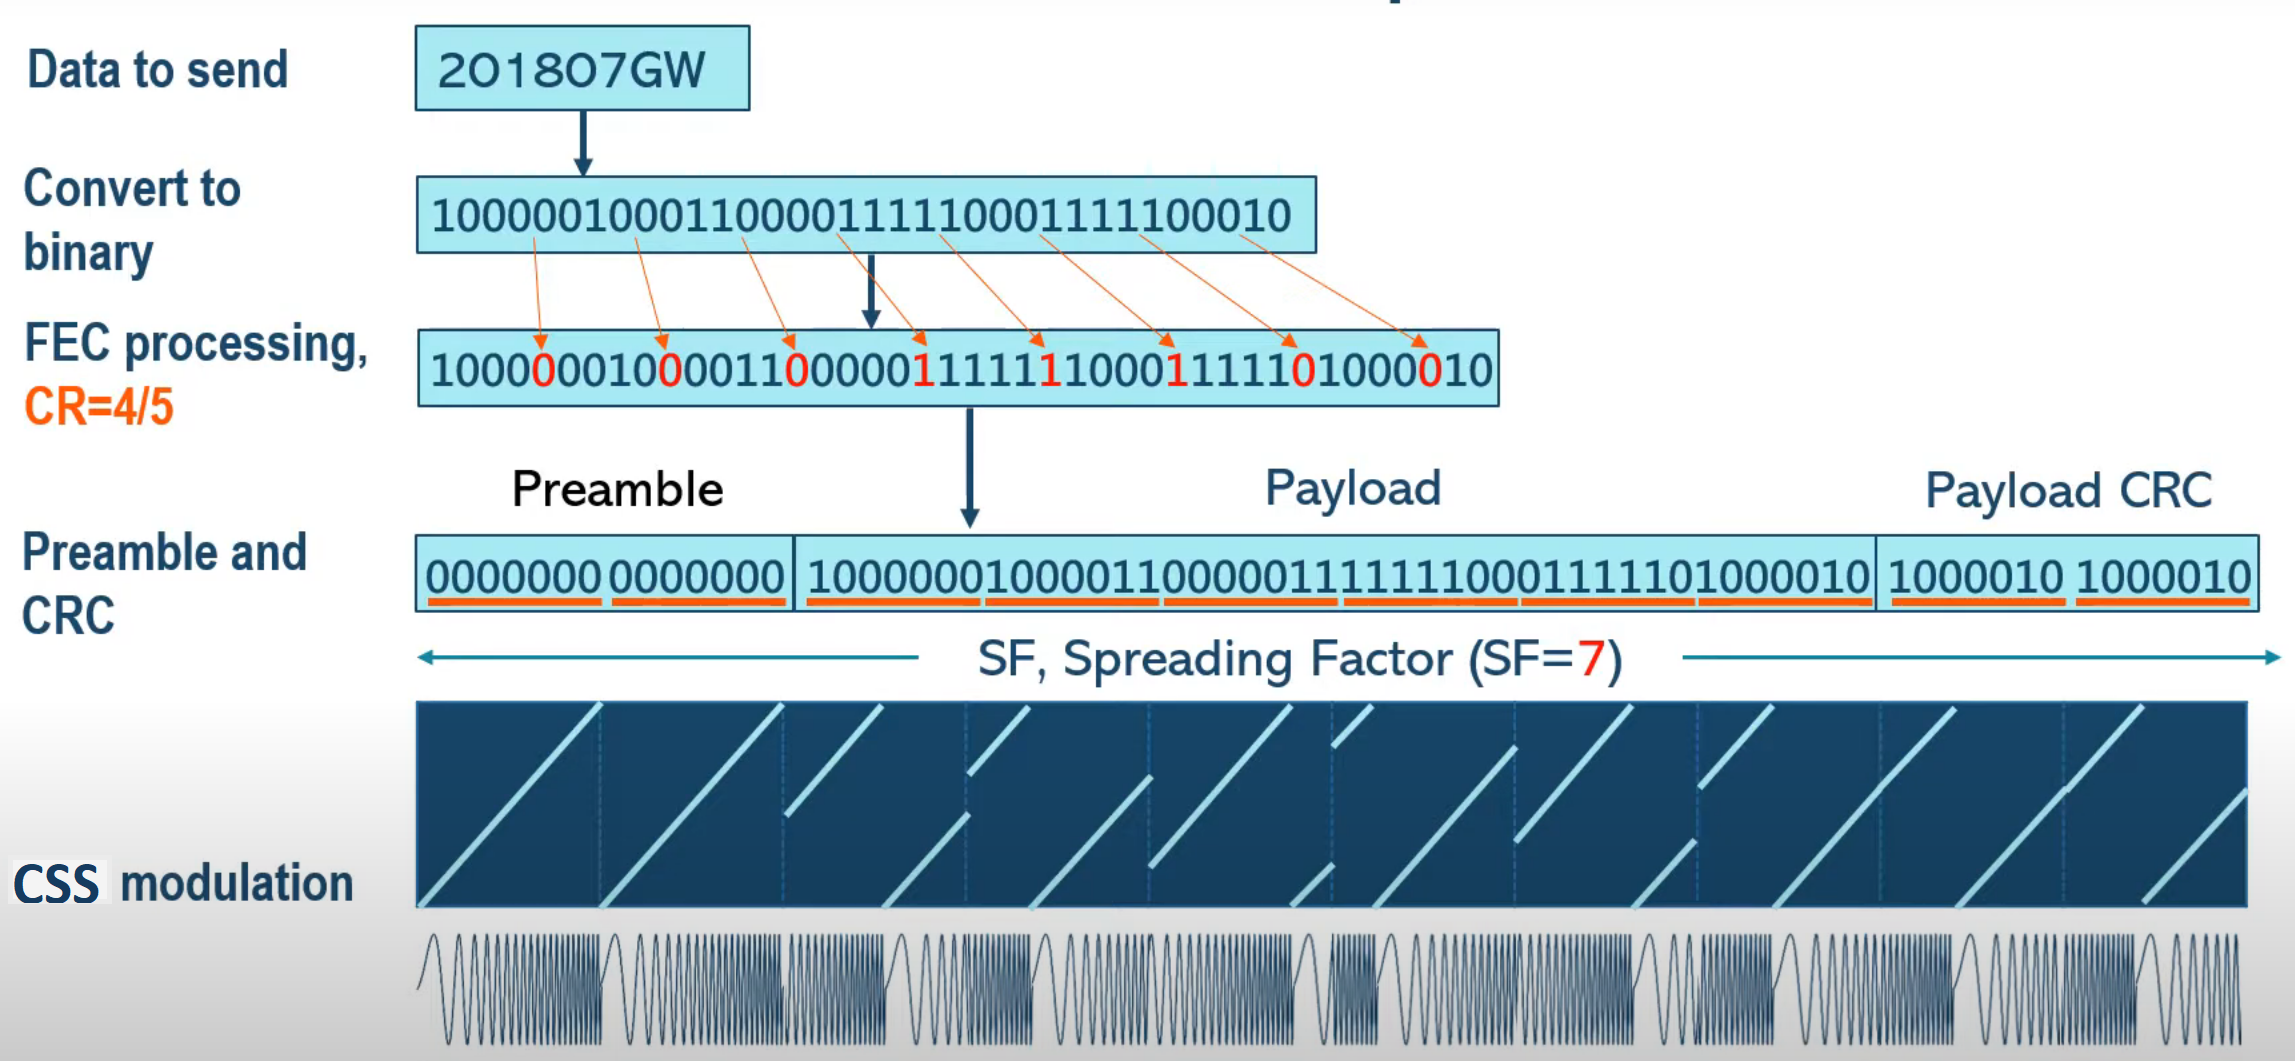
\includegraphics[width=1\textwidth]{Figures/loraModulation2.png}
	\caption{Proces spracovania odosielaných dát v LoRa (Binárne hodnoty su ukážkové, nezodpovedajú reálnej konverzií). \cite[Prevzaté z video prezentácie výrobcu GW Instek]{loratester}}
	\label{fig:loraModulation}
\end{figure}

\section{LoRa paket}
Štruktúra LoRa paketu môže byť závislá od daného použitia. Bežné sa ale stretávame s LoRa paketom, zloženým z preambuly, dát a kontrolného súčtu. Pričom maximálna 
povolená dĺžka dát je 255 bajtov.

Preambula slúži na synchronizáciu prijímacieho zariadenia. Je tvorená niekoľkými opakovaniami prázdneho chirp signálu, ktorý predstavuje symbol s hodnotou 0. 
Dĺžka preambuly, tzn. počet opakovaní prázdneho chirp signálu, je stanovená konfiguráciou zariadenia. Bežne sa stretávame s dĺžkou preambuly 8.
Na Obr. \ref{fig:loraModulation} môžme vidieť, že na preambulu boli použité iba 2 prázdne chirp signály -- teda dĺžka preambuly je 2.

Prijímacie zariadenie číta prijaté symboly v určitom časovom intervale -- okne. Tento interval sa ale nemusí zhodovať s intervalom, ktorý bol použitý pri vysielaní daných symbolov.
Je preto potreba synchronizovať prijímacie zariadenie aby hodnoty symbolov boli správne interpretované.

Zariadenie po prijatí nového paketu očakáva, že na začiatku paketu bude preambula definovanej dĺžky. Ak z paketu prečíta počet symbolov rovnakej hodnoty, zhodný 
s definovanou dĺžkou preambuly, predpokladá že sa jedná o preambulu a synchronizuje čítacie okno tak aby bolo zarovnané so symbolmi preambuly. Tzn. tak, aby symboly preambuly boli 
prečítané ako symbol 0.

Zjednodušené znázornenie procesu čítania symbolov a posun čítacieho okna môžme vidieť na Obr. \ref{fig:loraPreamble1}.

\begin{figure}[h!]
	\centering
	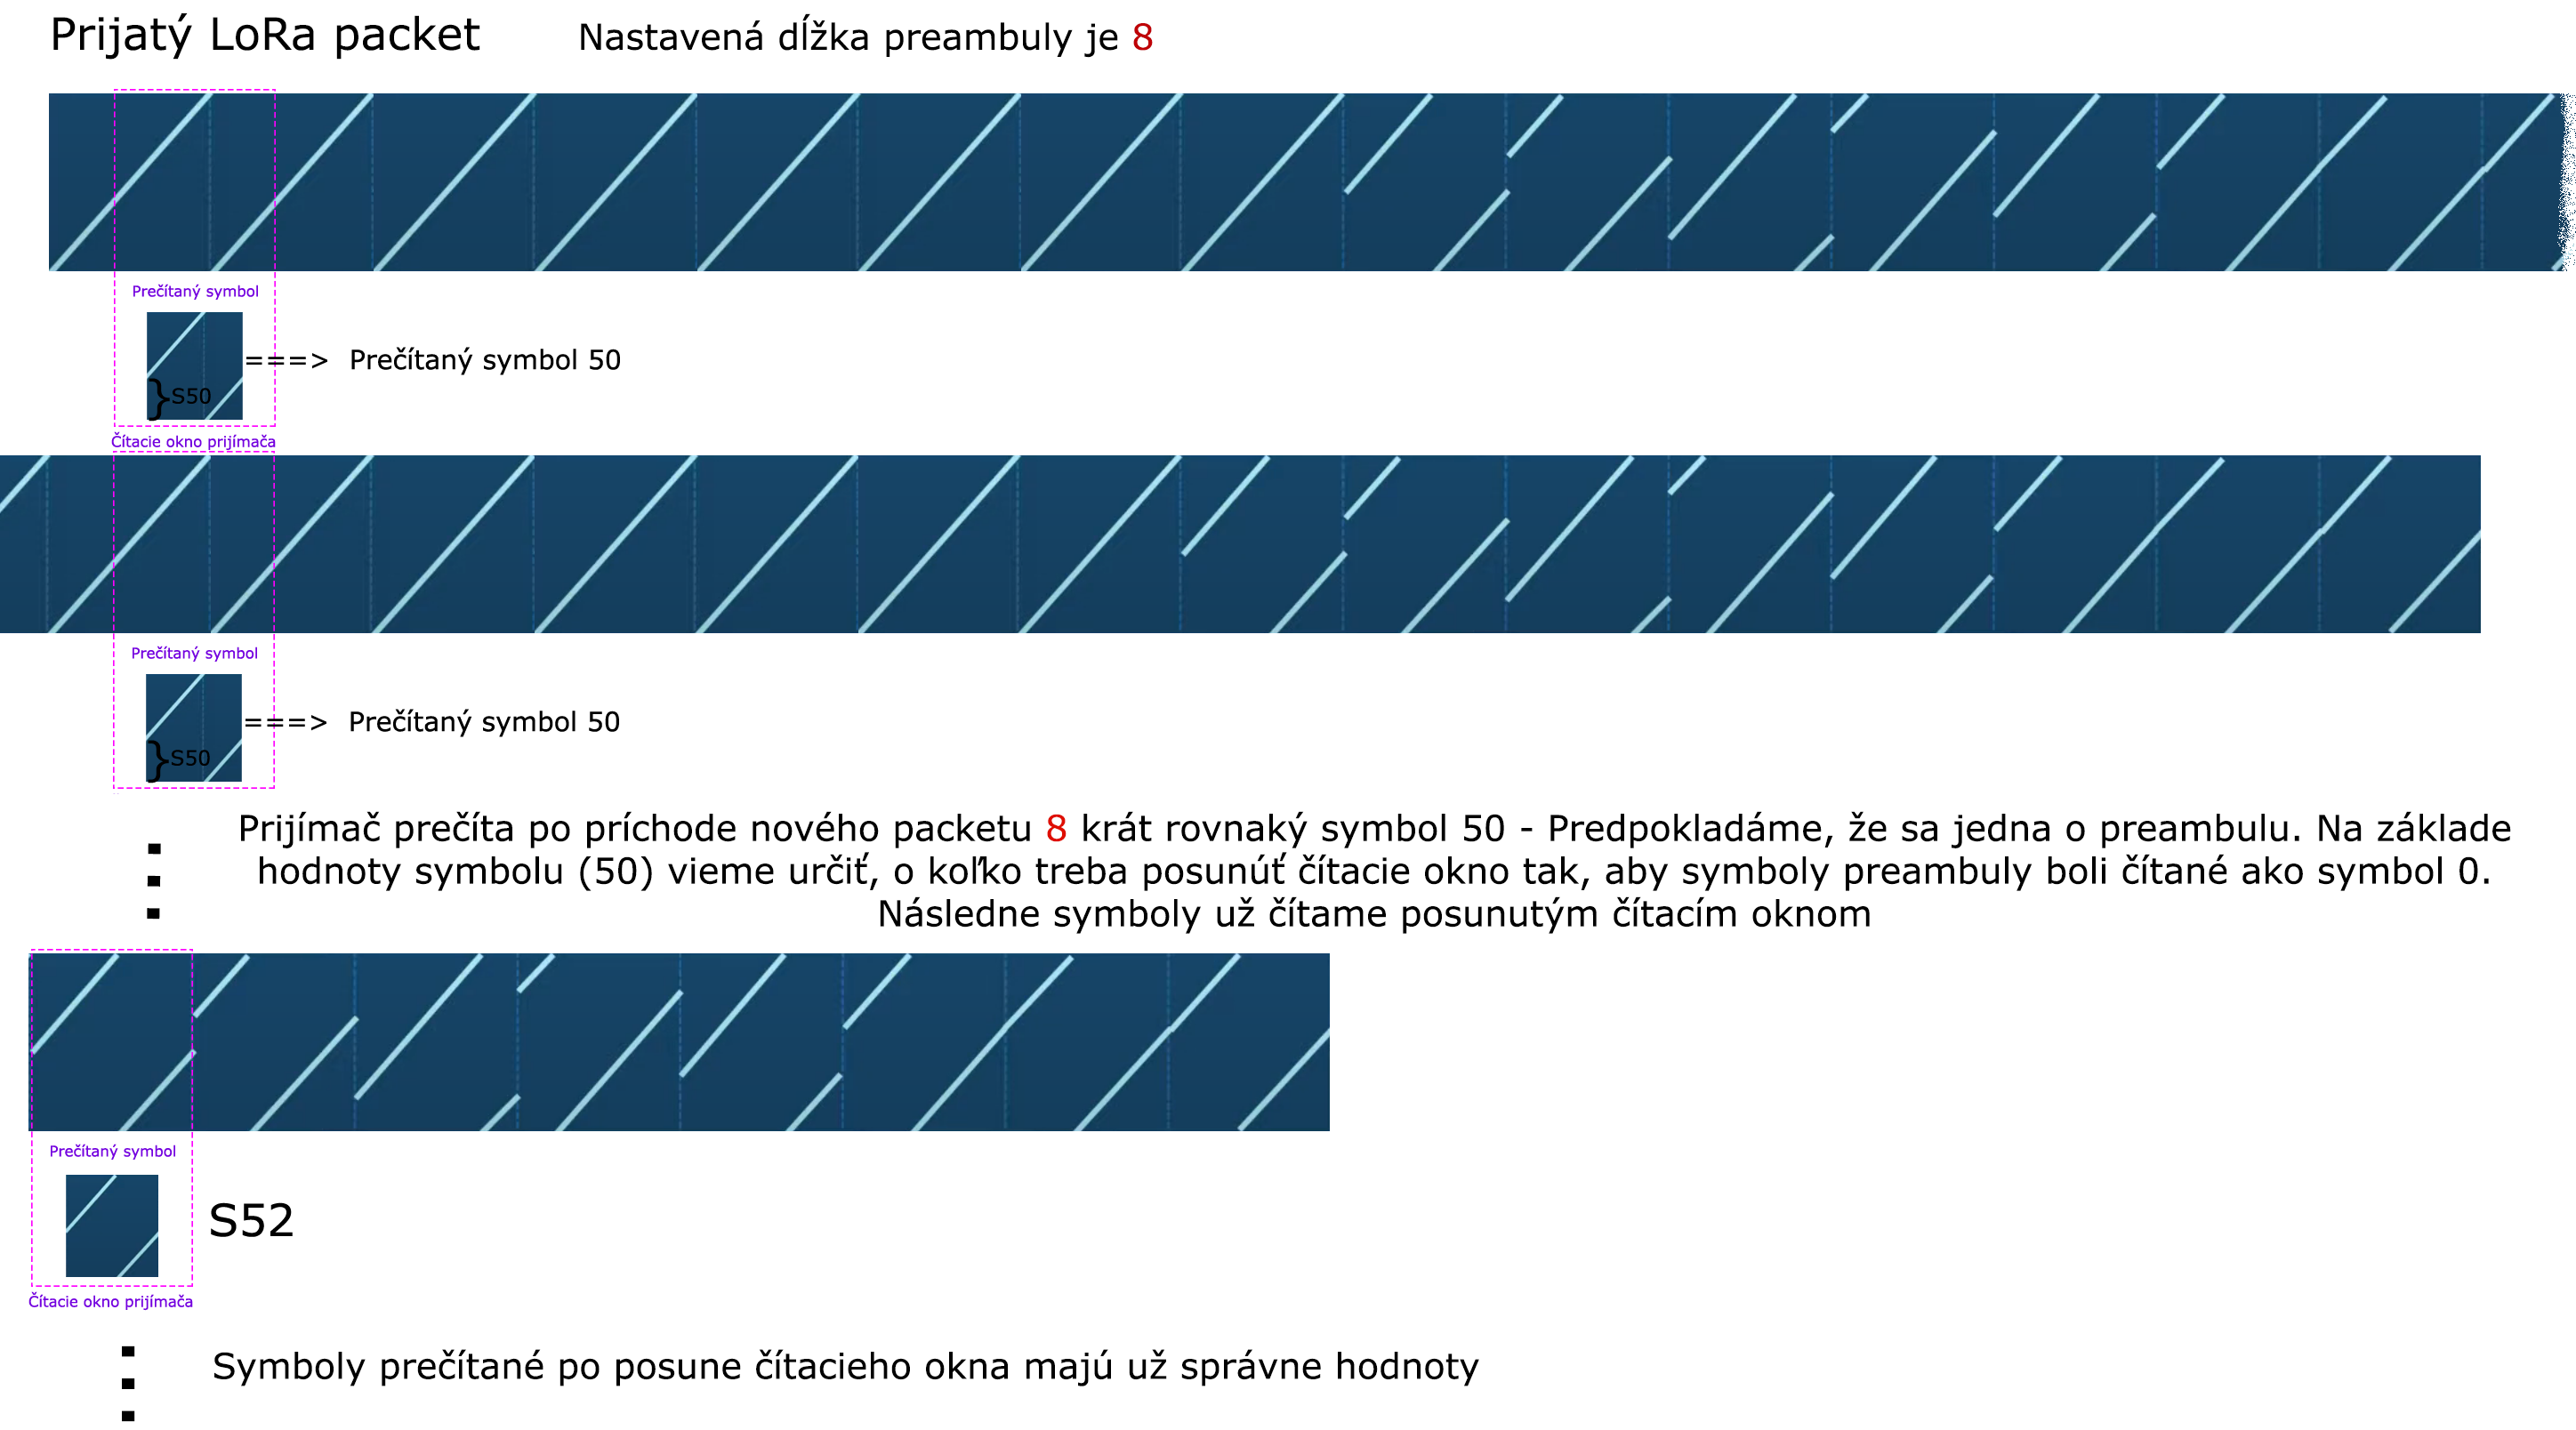
\includegraphics[width=1\textwidth]{Figures/preambulaSmall.png}
	\caption{Čítanie symbolov preambuly prijatého paketu a synchronizácia čítacieho okna na základe posunu preambuly.}
	\label{fig:loraPreamble1}
\end{figure}

\newpage
\section{LoRa parametre}
Pri používaní technológie LoRa je nutné správne zvoliť parametre na bezdrôtový prenos. Medzi nastaviteľné parametre patrí frekvencia, šírka pásma, rozprestierací factor a kódovací pomer.
Použitá frekvencia je závislá od regiónu, v ktorom chceme technológiu LoRa využívať, viď Tabuľka \ref{tab:ismBands}. 

V Európe je možné mimo 866 MHz pásma používať na LoRa aj 433 MHz pásmo. Okrem toho existuje ešte globálne používaná frekvencia 2,4 GHz. Tu sme ale limitovaní 
podporou daných frekvencií v nami použitom LoRa modeme. Bežné používané moduly, zväčša nemajú podporu pre 2,4 GHz frekvenčné pásmo.

\begin{table}[h!]
	\centering
  \small
  \setlength\tabcolsep{6pt}
	\caption[Frekvenčne pásma používane pre LoRa]{Frekvenčne pásma používane pre LoRa}
  \begin{tabular}{c|c}
    \toprule
    Región & Frekvenčné pásmo (MHz)\\
    \midrule
    Ázia & 433 \\
    Európa, Rusko, India, Afrika & 863--870 \\
    Severná Amerika & 902--928 \\
    Austrália & 915--928 \\
    Kanada & 779--787 \\
    Čína & 779--787, 470--510 \\
    \midrule
  \end{tabular}
  \label{tab:ismBands}
\end{table}
\newpage

Ostatné LoRa parametre sú vyberané na základe toho ako ďaleko, ako spoľahlivo a ako rýchlo je potrebné dáta prenášať. Je nutné zvoliť vhodný kompromis medzi rýchlosťou prenosu 
a dosahom prenosu. Pri výbere parametrov je ale taktiež potrebné dbať na to, aby nebol prekročený povolený kľučovací pomer. O tom si povieme viac v sekcii legislatíva.

Parameter bandwidth (BW) určuje šírku pásma, v ktorom sa bude chirp posúvať. Pri vyššej šírke pásma sa zvyšuje rýchlosť prenosu, avšak znižuje sa použiteľný dosah.
Najbežnejšie používané šírky pásma sú 125 kHz, 250 kHz a 500 kHz.

Rozprestierací faktor -- spreading factor (SF) určuje koľko bitov dát bude prenesených v každom vysielanom symbole. To určuje ako rýchlo sa chirp posúva po frekvenčnom pásme a tym pádom 
zvyšuje alebo znižuje rýchlosť prenosu na úkor zníženia alebo zvýšenia dosahu prenosu. Spreading factor je vo väčšine prípadov možné zvoliť z intervalu 6--12. 
Avšak niektoré LoRa modemy umožňujú nastaviť aj nižšie hodnoty rozprestieracieho faktoru. 

Používanie rozprestieracích faktorov prináša výhodu v podobe ortogonality správ vysielaných s rôznymi rozprestieracími faktormi. 
To znamená, že prijímač dokáže správne prijať a dekódovať správu poslanú s rozprestieracím faktorom X aj 
keď sa vysielaná správa časovo prekrýva s inou vysielanou správou s iným rozprestieracím faktorom Y.

LoRa obsahuje korekciu chýb spôsobených rušením. Využíva k tomu samo-opravný kód -- forward error correction (FEC), pri ktorom 
sa ku prenášaným dátam pridávajú korekčné bity. Tieto bity sú potom na prijímacej strane použité na detekciu a prípadnú opravu chyby ak k nejakej došlo vplyvom rušenia.
K nastaveniu korekcie chýb slúži parameter kódovací pomer -- coding rate (CR).

V technológií LoRa máme na výber zo štyroch možností pre parameter coding rate: 4/5, 4/6, 4/7 a 4/8. 
Označenie vyjadruje pomer bitov, ktoré nesú informáciu, ku bitom, ktoré budú reálne použité na prenos informácie. 
Napríklad pri kódovacom pomere 4/5 sa na každé 4 bity informácie pridáva 1 korekčný bit.
Vyšší kódovací pomer zabezpečí spoľahlivejší prenos dát ak sa nachádzame v rušivom prostredí, avšak zníži rýchlosť prenosu dát, 
pretože ku prenášaným dátam pridáva navyše dáta potrebné na korekciu chýb.

Rýchlosť prenosu dát (Data rate -- DR) môžme vyjadriť vzťahom:
\begin{figure}[h!]
  \centering
  \[DR = SF * \frac{\frac{4}{4+CR}}{\frac{2^{SF}}{BW}} *1000 \]
  \begin{tabular}{c c}
    DR & rýchlosť prenosu dát v bitoch za sekundu\\
    BW & šírka pásma v kHz \\
    SF & rozprestierací faktor (hodnoty 6--12) \\
    CR & kódovací pomer (hodnoty 1--4) \\
  \end{tabular}
\end{figure}

\section{LoRaWAN}
Technológia LoRa je definovaná len na fyzickej vrstve. Na používanie LoRa v IoT sieťach sú však potrebné aj vyššie vrstvy sieťového modelu.
K tomu vznikol protokol LoRaWAN \cite{lorawan}, ktorý je spravovaný organizáciou LoRa Alliance \cite{lora}.

LoRaWAN definuje komunikačný protokol a architektúru IoT sieti. Siete používajú hviezdicovú topológiu, prípadne topológiu hviezdu hviezd, kde 
centrálnym uzlom je LoRaWAN brána -- gateway, ktorá je pripojená k internetu a pevnému napájaniu. Ostatné uzly siete posielajú dáta do tejto brány, 
ktorá ich potom preposiela na internet. Tam sú už dáta dostupné odkiaľkoľvek.

LoRaWAN definuje tri základne triedy zariadení, ktoré sa v sieti vyskytujú. Triedy špecifikujú funkciu zariadenia a jeho vlastnosti.
Sú nimi triedy A, B a C, kde do triedy A spadajú zariadenia väčšinou poháňané batériami, ktoré po odvysielaní svojich dát otvárajú dve prijímacie okna, 
v ktorých čakajú na príjem dát z brány.
Trieda B je rozšírením triedy A. Zariadenia v tejto triede môžu otvárať dodatočné prijímacie okna v naplánovaných časových intervaloch.
Zariadenia z triedy C môžu prijímať neustále. Z tohto dôvodu majú vyššiu spotrebu energie a zvyčajne su pripojené k stálemu napájaniu.

Zariadenia používané na realizáciu gateway bývajú zväčša výkonnejšie oproti koncovým zariadeniam. Okrem toho su schopné prijímať na viacerých frekvenciách a
LoRa parametroch zároveň. Gateway môže byť pripojená ne nejakú cloudovú službu, cez ktorú je možne spravovať zariadenia v sieti. Medzi najznámejšie 
služby patrí The Things Network (TTN) \cite{ttn}. Je však možné spojiť LoRaWAN aj s inými populárnymi cloudovými službami ako je napríklad Microsoft Azure \cite{azure} 
alebo Google Cloud \cite{googleCloud}.

\section{Legislatíva}
V Európe sa k frekvenčnému pásmu používaného pri technológií LoRa viažu určité obmedzenia. 
Obmedzenia sa týkajú používania fyzického média. Regulácia určuje maximálnu povolenú dobu, v ktorú môže vysielač na daných frekvenciách vysielať 
v rámci jednej hodiny a maximálny vysielací výkon, akým môže signal vysielať.

Určuje sa takzvaný klučovací pomer, ktorý hovorí koľko percent času z nejakého celkového času môže vysielač vysielať.
Ak by zariadenie vysielalo signál po dobu jednej jednotky času z celkových 10 jednotiek času, tak kľučovací pomer by bol 10 \%.

Český Telekomunikačný úrad stanovuje vo všeobecné oprávnění č. VO-R/10/07.2021-8 \cite{vor}, že 
frekvenčné pásmo, do ktorého spadá technológia LoRa, patrí do skupiny g. Pre túto skupinu je maximálny povolený kľučovací pomer 1 \% a maximálny 
vysielací výkon 25 mW (14 dBm). Znamená to teda, že zariadenia môžu každú hodinu vysielať maximálne po dobu 36 sekúnd.
Pre pásmo 869,40--869,65 MHz je ale udelená výnimka, ktorá umožňuje vysielať s kľučovacím pomerom 10 \% a maximálnym vysielacím výkonom 500 mW (27 dBm).

\chapter{Dostupné LoRa moduly }
Pri práci s technológiou LoRa máme na výber z rôznych modulov od rôznych výrobcov.
Moduly môžme rozdeliť podla použitia na moduly pre koncové zariadenia a moduly pre gateway.
Moduly pre koncové zariadenia obvykle dokážu prijímať a odosielať iba na jednom kanále ( kombinácia LoRa parametrov --  BW, SF, CR a frekvencia ) súčasne a majú 
nízku spotrebu energie. Moduly pre gateway dokážu prijímať a odosielať na viacerých kanáloch súčasne.

V tejto časti sa budeme zaoberať dostupnými modulmi pre koncové zariadenia.
Keďže je technológia LoRa patentovaná výrobcom Semtech \cite{semtech}, tak všetky dostupné LoRa čipy su práve od tohto výrobcu a moduly od iných výrobcov 
sú založené na používaní týchto čipov. Kompletné porovnanie parametrov najpouživanejších modulov je možné vidieť v tabuľke \ref{tab:semtechModules}.

\section{SX127x/SX126x}
Výrobca Semtech \cite{semtech}, prináša LoRa čipy -- modemy série SX127x a SX126x. Ponúkajú vysoký výkon za pomerne nízku cenu a ako sme už spomínali, ostatné LoRa moduly 
iba implementujú tieto LoRa modemy a rozširujú ich o ďalšiu funkcionalitu.

\subsection{SX127x}
SX127x LoRa modemy používajú LoRa modulačnú techniku frequency hopping spread-spectrum, patentovanú firmou Semtech.

Maximálny vysielací výkon týchto modemov je 100 mW.
Vďaka použitej modulačnej technike je možné dosiahnuť vysokej citlivosti modemov.
Výrobca uvádza citlivosť cez -137 dBm pri modemoch SX1272/73 a -148 dBm pri modemoch SX1276/78/79.


Modemy SX1272 a SX1273 ponúkajú menší link budget \footnotemark[1] 157 dB oproti 168 dB pri modemoch SX1276/77/78/79. 
\footnotetext[1]{Súčet zisku a strát signálu medzi vysielačom a prijímačom v bezdrôtovom prenose.}
\newpage
Majú menší rozsah frekvenčných pásiem medzi 860 a 1020 MHz oproti modemom SX1276/77/78/79, kde 
je možné vybrať frekvenčné pásma z rozsahu 137 až 1020 MHz.

Okrem toho majú aj vyššiu spotrebu energie.

\subsection{SX126x}

Modemy zo série SX126x - SX1261/62/68 sú nasledovníkmi predošlých modemov SX127x. Majú väčší vysielací výkon vďaka integrovanému zosilňovaču a menšiu spotrebu energie. 
Obsahujú precízny TCXO oscilátor, ktorý zabezpečuje presnejšie a stabilnejšie riadenie počas prevádzky modemu. Okrem LoRa modulácie obsahujú aj G(FSK) moduláciu, ktorá je vhodná pre staršie 
prípady použitia.

Modemy obsahujú +22/+15 dBm zosilňovač, vďaka ktorému majú vyšší link budget oproti modemom zo série SX127x. 
Ten je pri modemoch série SX126x výrobcom udávaný na 170 dBm, takže sú optimálne pre aplikácie vyžadujúce väčší dosah alebo robustnosť.

\begin{table}[!h]
	\centering
  \small
  \setlength\tabcolsep{4pt}
	\caption[Parametre Semtech SX modemov]{Parametre Semtech SX modemov}
  \begin{tabular}{c|c|c|c|c|c|c|c|c}
    \toprule
    Modem & Frekvencia & SF & BW (kHz) & Citlivosť & Spotreba \footnotemark[1] & Rozhranie & Výkon\footnotemark[2] & Cena\footnotemark[3]\\
    \midrule
    SX1272 & 860--1020 MHz & 6--12 & 125--500 & -137 dBm & 11,2 mA & SPI & 20 dbm & 9€ \\
    SX1273 & 860--1020 MHz & 6--9 & 125--500 & -130 dBm & 11,2 mA & SPI & 20 dbm & 7€ \\
    SX1276 & 137--1020 MHz & 6--12 & 7,8--500 & -148 dBm & 12 mA & SPI & 20 dbm & 10€ \\
    SX1277 & 137--1020 MHz & 6--9 & 7,8--500 & -139 dBm & 12 mA & SPI & 20 dbm & 7€ \\
    SX1278 & 137--525 MHz & 6--12 & 7,8--500 & -148 dBm & 12 mA & SPI & 20 dbm & 8€ \\
    SX1279 & 137--960 MHz & 6--12 & 7,8--500 & -148 dBm & 12 mA & SPI, UART & 20 dbm & 11€ \\
    \hline
    SX1261 & 150--690 MHz & 5--12 & 7,80--500 & -125 dBm & 8 mA & SPI & 15 dbm & 7€ \\
    SX1262 & 150--690 MHz & 5--12 & 7,80--500 & -125 dBm & 8 mA & SPI & 22 dbm & 8€ \\
    SX1268 & 410--810 MHz & 5--12 & 7,80--500 & -148 dBm & 4.6 mA & SPI & 22 dbm & 7€ \\
    \midrule
  \end{tabular}
  \label{tab:semtechModules}
\end{table}
\footnotetext[1]{Spotreba počas prijímania (mA)}
\footnotetext[2]{Maximálny vysielací výkon}
\footnotetext[3]{Cena platná ku Q4 2022}

\section{RFM9xW}
Moduly RFM95W/96W/98W od výrobcu HopeRF \cite{hoperf} implementujú SX LoRa modemy od výrobcu Semtech.
Jedná sa o jednoduchý modul, ktorý obsahuje všetku riadiacu elektroniku potrebnú pre riadenie Semtech LoRa modemu.
Okrem riadiacej elektroniky obsahuje modul aj zosilňovač signálu (+14 dBm), ktorý zvyšuje dosah bezdrôtového prenosu.

Existuje niekoľko verzií modulov RFM9xW, kde každá verzia používa iný semtech LoRa modem a zdieľa parametre daného modemu.

\section{Moduly a zariadenia použité v tejto práci}
Na vývoj a testovanie tejto práce boli použité rôzne zariadenia s rôznymi platformami. Na simulovanie jednoduchých koncových zariadení, 
ktoré môžu predstavovať napríklad nejaký senzor, boli použité mikrokontroléry TTGO od výrobcu LILYGO \cite{lilygo}.

Okrem mikrokontrolérov TTGO boli použité aj mikrokontroléry Raspberry Pi Pico a jednodoskový počítač Raspberry Pi.
Nami použité mikrokontroléry môžu byť neskôr rozšírene o batériu a stať sa tak mobilnými.

\subsection{TTGO LoRa32}
TTGO LoRa32 je multifunkčný mikrokontrolér postavený na module ESP32, ktorý poskytuje 
potrebné moduly pre bezdrôtovú komunikáciu, vrátane Wi-Fi, Bluetooth a SX1276 LoRa modulu. 

Tento mikrokontrolér je špeciálne navrhnutý pre projektovanie internetu vecí (IoT), senzorov a ďalších podobných aplikácií, 
ktoré vyžadujú spoľahlivú a energeticky úspornú bezdrôtovú komunikáciu.

Jednou z výhod tohto mikrokontroléru je jeho úsporný režim spánku, ktorý umožňuje znížiť spotrebu až na 0,6 mA. 
Tento režim je ideálny pre aplikácie, ktoré potrebujú byť v prevádzke čo najdlhšie, bez nutnosti pravidelného nabíjania batérie.

Okrem toho TTGO LoRa32 obsahuje aj 0,96 palcový čiernobiely displej pripojený cez I2C rozhranie. 
Tento displej môže slúžiť ako zobrazovací panel pre aplikácie, ktoré potrebujú zobrazovať textové a grafické informácie.

\subsection{TTGO T-Beam}
Tento mikrokontrolér je taktiež založený na module ESP32 a obsahuje Wi-Fi, bluetooth a LoRa modul.
Rovnako používa SX1276 LoRa modem no okrem spomínaných modulov obsahuje aj GPS modul.

Mikrokontrolér ma na zadnej strane držiak na batériu, z ktorej môže byť napájaný a taktiež aj nabíjací modul 
pre bezpečné nabíjanie a ochranu lítiových batérií.
V režime spánku ma spotrebu 0,2 mA. Podporuje pripojenie dodatočného displeju, avšak nami používaný mikrokontrolér tento displej nemal.

Na Obr \ref{fig:ttgo-moduly} môžeme vidieť oba mikrokontroléry TTGO.
\begin{figure}[h!]
  \centering
  \subfloat[\centering TTGO LoRa32]{{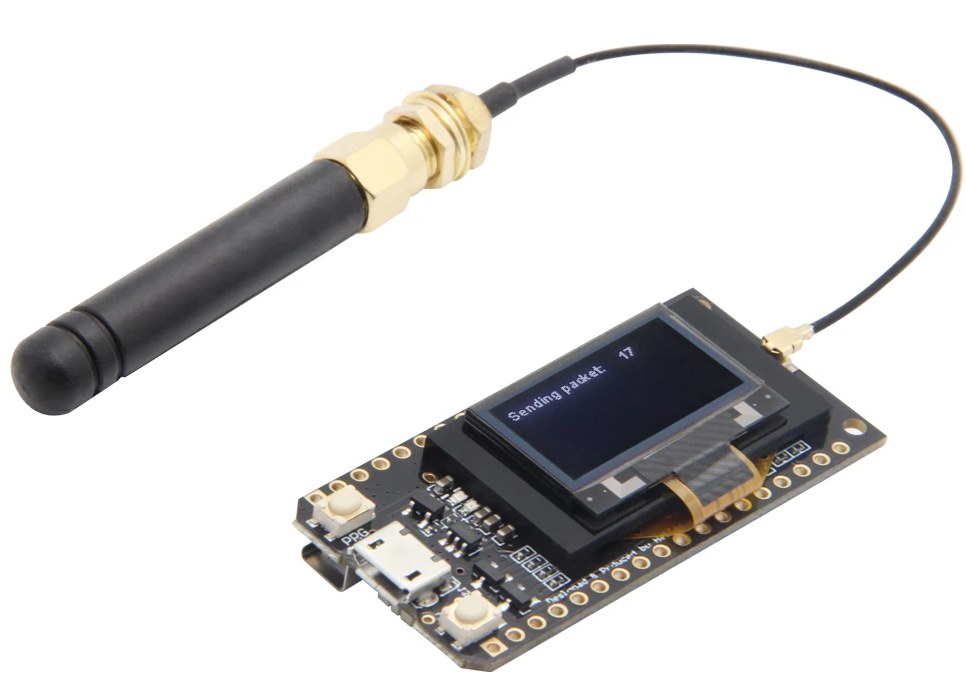
\includegraphics[width=0.4\textwidth]{Figures/LILYGO-TTGO-LoRa32-V1.png} }}
  \qquad
  \subfloat[\centering TTGO T-beam]{{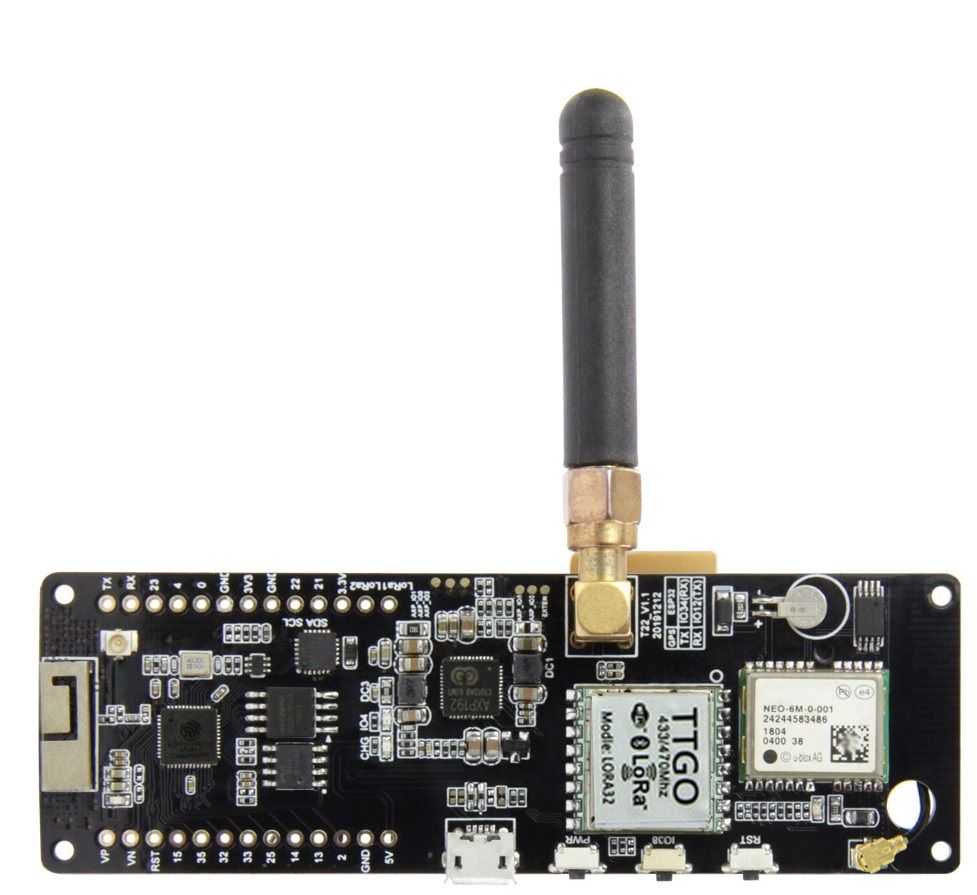
\includegraphics[width=0.35\textwidth]{Figures/ttgo-tbeam.jpg} }}
  \caption{Mikrokontroléry TTGO. Prevzaté z \cite{lilygo}}
  \label{fig:ttgo-moduly}
\end{figure}
\newpage

\subsection{Raspberry Pi Pico RP2040}
Mikrokontrolér od známej organizácie Raspberry Pi \cite{rpiOrg}, založený na dvoj-jadrovom ARM procesore. 
Existuje verzia s Wi-Fi modulom aj bez. Na programovanie sa využíva jazyk C alebo MicroPython, 
prípadne derivát MicroPythonu -- CircuitPython. V tejto práci bol použitý práve CircuitPython.

Avšak aby bolo možné využívať tieto mikrokontroléry s technológiou LoRa, bolo potrebné pridať k nim nejaký LoRa modul.

Na implementáciu v tejto práci boli preto zvolené zariadenia Armachat, ktoré kombinujú mikrokontrolér Raspberry Pi Pico s LoRa modulom RFM96W.
Okrem toho pridávajú dvoj palcový farebný displej a klávesnicu.

Ako toto zariadenie vyzerá môžme vidieť na Obr \ref{fig:armachat}.

\begin{figure}[h!]
	\centering
	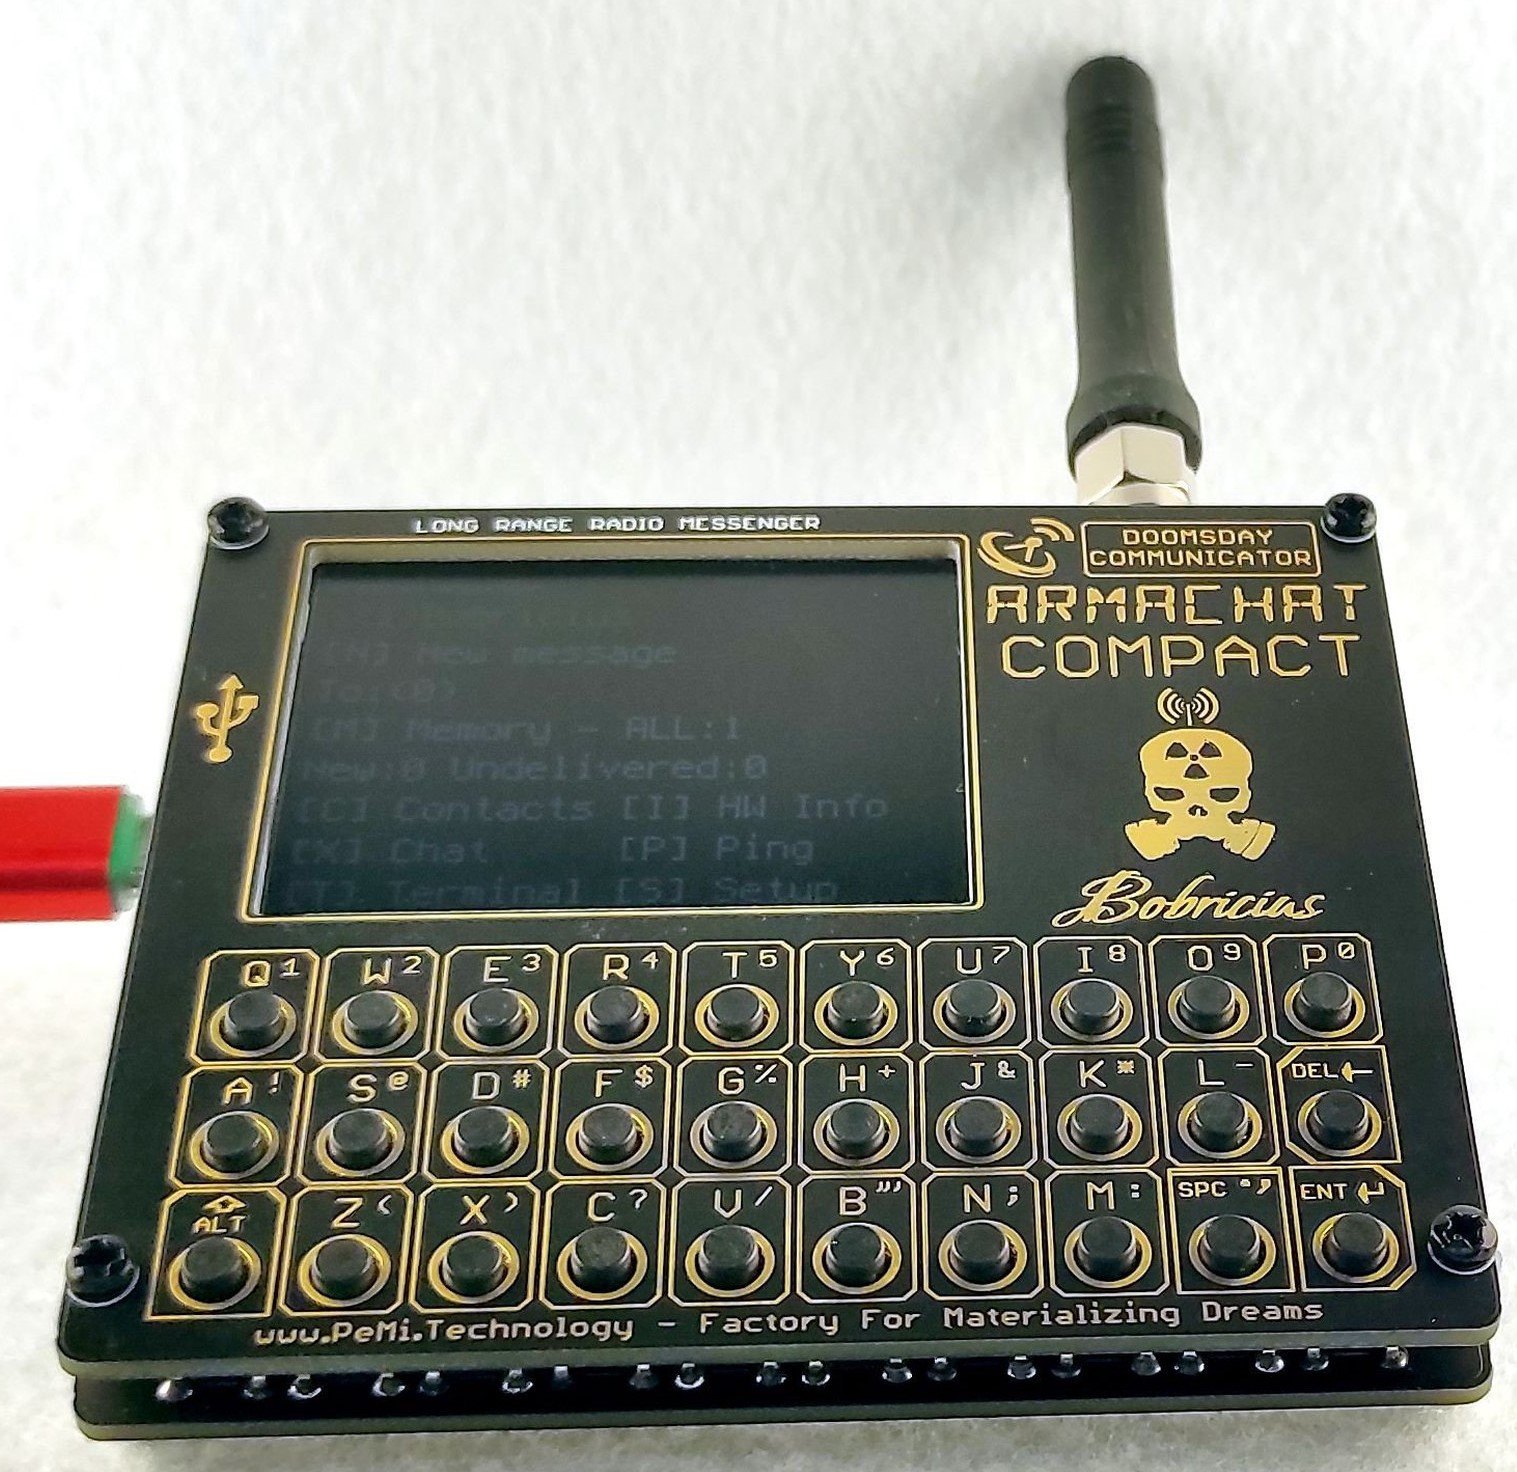
\includegraphics[width=0.4\textwidth]{Figures/armachat.jpg}
	\caption{Zariadenie Armachat. Prevzaté z \cite{armachatObr}}
	\label{fig:armachat}
\end{figure}

\subsection{Raspberry Pi 2B}
Jednodoskový, štvor-jadrový počítač vytvorený organizáciou Raspberry Pi. 
Toto zariadenie obsahuje eternetový port, ktorý môže slúžiť na pevné pripojenie do internetovej siete.
Počítač sam o sebe neobsahuje žiaden modul a tak bol pre prácu s LoRa pridaný RFM96W modul, pripojený do vstupno-výstupných pinov počítača.

Na pripojenie bola použitá SPI zbernica. Raspberry Pi ponúka dva SPI porty, v našom prípade bol použitý ten prvý na pinoch 11, 10, 9 a 8.

Na rozdiel od predchádzajúcich mikrokontrolérov disponuje tento jednodoskový počítač oveľa väčším výkonom a pamäťou, 
avšak ma oveľa vyššiu spotrebu energie. Z tohto dôvodu tento počítač plnil rolu nemobilného uzlu v sieti, ktorý bol pripojený cez ethernet do internetovej siete.

Vďaka tomu, že CircuitPython je možne spojazdniť aj na Raspberry Pi, bolo možné čast implementácie zdielať medzi Raspberry Pi Pico a Raspberry Pi 2B.


\chapter{Existujúce riešenia}
Téma mesh sietí je v tejto dobe veľmi aktuálna a vývojári sa snažia vytvoriť rôzne riešenia, ktoré by nahradili aktuálne používane 
prístupy topológie hviezda v IoT sieťach. 

V rámci sieťového prenosu je kľúčové zabezpečiť správne smerovanie, aby správy mohli byť úspešne doručené 
od odosielateľa k príjemcovi. Je k dispozícii celé množstvo rôznych smerovacích algoritmov, ktoré môžu byť využité 
s cieľom dosiahnuť tento cieľ, pričom každý z nich prináša svoje výhody a nevýhody \cite{ALOTAIBI2012940}. Preto je dôležité zvážiť 
konkrétne požiadavky a okolnosti siete a zvoliť ten najlepší algoritmus pre danú situáciu

Použitie mesh topológie môže so sebou prinášať rôzne výhody oproti bežne zaužívaným topológiam typu hviezda.
Vo výskume od Ochoa et al. \cite{8115793} porovnávali spotrebu energie medzi 
topológiou typu mesh a hviezdicovou topológiou v sieti LoRa. A z týchto štúdií možno vyvodiť, že pre rozsiahlejšie siete je viac
efektívnejšie, z hľadiska spotreby energie, použiť topológiu mesh. 

Okrem toho je možné optimalizovať výber rádiových nastavení v súlade s hustotou siete tak, 
aby sa v mesh sieťach ešte viac optimalizovala spotreba energie.


Existujú rozvinuté projekty ako napríklad Meshtastic \cite{meshtastic}, ktorý sa snaží vytvoriť rozsiahlu decentralizovanú mesh sieť na miestach bez inej dostupnej konektivity, 
za použitia lacných zariadení.

Ďalším zaujímavým projektom je Armachat \cite{armachat}, ktorý ponúka možnosť komunikácie v prípade nedostupnosti ostatných sieti, napríklad po nejakej prírodnej alebo inej katastrofe.
Súčasťou projektu Armachat sú plošné spoje, z ktorých si používateľ poskladá finálne zariadenie.
Zariadenia Armachat su poháňané mikrokontrolérmi Raspberry Pi Pico, obsahujú LoRa moduly, displej, klávesnicu a ďalšie vymoženosti.

Originálny projekt avšak sám o sebe zatiaľ nepodporuje využívanie mesh topológie. Používa ale rovnakú štruktúru správ ako projekt Meshtastic a vďaka tomu je možné 
v projekte Armachat využívať mesh sieť projektu Meshtastic.

Teoretických návrhov ako realizovať smerovanie v mesh sieťach je mnoho, avšak v praxi sa najčastejšie stretávame s 
distance vector smerovaním alebo flooding prístupom. Najzaujímavejšie riešenia si bližšie popíšeme 
v následujúcich sekciách.

\section{LoRa mesher}
LoRaMesher \cite{loramesher} je C++ knižnica, ktorú je možné použiť na komunikáciu v LoRa mesh sieťach.

Na smerovanie v sieti používa distance vector routing protokol. Tento protokol vyberá cestu, kadiaľ bude správa v sieti preposlaná od odosielateľa k príjemcovi, na základe 
najlepšej cesty. Najlepšiu cestu definuje ako cestu s najmenším počtom hopov -- preskokov medzi uzlami v mesh sieti.

K realizácií distance vector smerovania je potrebné udržiavať smerovaciu tabuľku, ktorá obsahuje informácie o ID uzlov, cez ktoré susedné uzly sa dané uzly dajú dosiahnuť a 
koľko preskokov bude potrebných na dosiahnutie týchto uzlov. Smerovacia tabuľka je periodicky aktualizovaná cez špeciálny typ správ, ktoré sú odosielané 
všetkými uzlami v sieti. Túto smerovaciu tabuľku si drží a priebežne aktualizuje každý uzol v sieti.

LoRaMesher používa FreeRTOS, čo je operačný systém reálneho času. Takéto operačné systémy garantujú dokončenie úloh v určitom čase.
FreeRTOS je použitý na zabezpečenie plánovania úloh. Rozličné úlohy sa starajú o prijatie a odoslanie paketov, iné úlohy sa starajú o samotne 
spracovanie prijatých paketov.

LoRaMesher dokáže nájsť novo vytvorené uzly v sieti vďaka smerovaciemu protokolu. Pri odoslaní správ čaká na prijatie potvrdzujúcej ACK správy, ktorá potvrdzuje, 
že správa bola prijatá a tým zaisťuje spoľahlivosť. Správy väčšie ako 222 bajtov rozdeľuje na viacero správ, ktoré pošle postupne.

\section{Meshtastic}
Meshtastic vytvára mesh sieť za použitia lacných mikrokontrolérov s LoRa modulmi.
Myšlienka tohto projektu spočíva v tom, že vytvára komunikačnú sieť na miestach kde neexistuje spoľahlivá infraštruktúra na bezdrôtovú komunikáciu (napr. v horách).

Posielanie správ v sieti je založené na jednoduchom multi-hop flooding.
Každý uzol znovu odvysiela paket, ktorý prijal ( pokiaľ nedošiel počet preskokov na 0 ), až kým sa paket nedostane do určenej destinácie naprieč mesh sieťou.
Prenášane správy su šifrované za pomoci šifrovacieho algoritmu AES.

Zariadenia používane v projekte Meshtastic majú okrem LoRa modulu zabudovaný aj bluetooth modul, vďaka ktorému je možne sa k zariadeniu pripojiť cez mobilný telefón, ktorý slúži ako rozhranie pre 
užívateľa. Cez aplikáciu v mobilnom telefóne môže používateľ vytvárať a prijímať správy. Správy sa cez bluetooth prenášajú z telefónu do zariadenia kde sa následne odošlú cez 
LoRa do siete.

Meshtastic poskytuje možnosť pripojenia sa k oficiálnemu meshtastic mqtt brokerovi. Toto umožňuje prepojiť malé lokálne mesh siete do väčšej globálnej siete a 
tak rozšíriť dosah siete.

\section{LoRaBlink}
Ďalší multi-hop protokol, ktorý používa časovú synchronizáciu medzi uzlami. Časová synchronizácia definuje sloty, v ktorých môže uzol pristupovať ku prenosovému médiu a 
vysielať svoje dáta. Správy sa sieťou šíria pomocou multi-hop flooding.

Sieť sa skladá z jedného uzlu, ktorý plní rolu takzvaného datasinku (gateway alebo brána) a ostatných uzlov. Uzly siete posielajú dáta do datasinku alebo dáta z neho prijímajú.

V určitých intervaloch datasink vyšle tzv. beacon signál. Tento signál slúži na časovú synchronizáciu medzi uzlami a značí začiatok novej epochy. 
Každá epocha obsahuje N slotov, v ktorých môžu uzly vysielať dáta. Beacon správa obsahuje hop count, ktorá udáva vzdialenosť ku datasinku.
Ked nejaký uzol príjme beacon signál, vyšle svoj vlastný beacon signál v ďalšom volnom slote, ktorý vyberá na základe vzdialenosti od datasinku (hop count).

Ked uzol potrebuje poslať nejaké dáta, tak vyberie najskorší volný slot a v nom vysiela svoje dáta. Ak tieto dáta príjme uzol, ktorý nie je datasink a 
hop count daného uzlu ku sinku je menší ako hop count vysielacieho uzlu, tak dáta v ďalšom volnom slote znovu prepošle. Toto sa opakuje, až 
kým dáta nedosiahnu datasink.

Takto tvorená sieť avšak vyžaduje existenciu nejakého hlavného uzlu (datasinku), ktorý je potrebný na riadenie siete prostredníctvom časovej synchronizácie.

\section{Pymesh}
Pymesh je súčasťou Pycom \cite{pycom} ekosystému. Tento ekosystém je určený na vývoj IoT systémov. Ponúka rôzne zariadenia, ktoré su určené na použitie s týmto 
ekosystémom. Zariadenia obsahujú WiFi, bluetooth a LoRa, prípadne SigFox moduly. Zariadenia je možné rozšíriť o rôzne moduly so senzormi, ktoré rozširujú ich schopnosti.

PyMesh sieť sa skladá z uzlov, ktoré môžu vystupovať v rôznych roliach. Sú nimi Border Router, Leader, Router a Child. Uzly typu gateway su označované ako Border Routers a prepájajú LoRa sieť s 
internetom. Uzly typu router slúžia len na preposielanie paketov ďalej. Leader alebo koordinátorske uzly sú zodpovedné za vytváranie a správu siete a Child uzly sú koncové 
zariadenia.

Uzly v sieti môžu komunikovať ad-hoc. V sieti môže dojsť k situácií kedy bude chcieť viacero uzlov vysielať v rovnakom čase a došlo by tak ku kolízií.
Aby sa zabránilo takýmto situáciám, je použitá metóda Listen Before Talk, pri ktorej sa pred vysielaním signálu overí, či nie je v sieti už niekto iný, kto by práve 
vysielal. Pokiaľ áno, tak sa posielaná správa vyšle neskôr.

PyMesh je primárne určený na použitie s Pycom zariadeniami a použitie na inom zariadení by vyžadovalo väčšie úpravy zdrojového kódu.

Na smerovanie paketov v sieti využíva kombináciu dvoch prístupov. Ak chce uzol vyslať nejaký paket a destinácia toho paketu je v dosahu daného uzla, tak sa paket priamo odošle. 
Pokiaľ ale destinácia nie je v dosahu, uzol najskôr vyšle požiadavok na vytvorenie trasy ku destinácií všetkým svojím susedom. Títo susedia to prepošlú ďalej svojím susedom. 
Takto sa bude paket preposielať, až kým sa nedostane ku uzlu, ktorého susedom je hľadaná destinácia prípadne destinácia samotná. Následne sa nájde najkratšia cesta ku destinácii a táto cesta sa uloží do smerovacích 
tabuliek uzlov. Následne môže uzol vyslať pôvodný paket do destinácie.


\section{Synchronous LoRa Mesh}
Projekt Synchronous LoRa Mesh \cite{synchronouslorameshnetwork} vznikol z potreby získavania real-time dát z podzemných kanalizácií. Tieto dáta sú potrebné k monitorovaniu a predikcií kritických situácií akými 
sú napríklad záplavy.

LoRaWAN však nemá moc veľký dosah do podzemia. Z toho dôvodu by bolo potrebné v podzemných priestoroch implementovať LoRaWAN gateway-e, ktoré su ale energeticky náročne, drahé a vyžadujú 
pevné pripojenie do elektrickej a prípadne aj internetovej siete, ktoré v kanalizáciách niesu dostupné. Okrem toho, by museli byť všetky ostatné uzly v podzemnej sieti v dosahu danej gateway a pri väčšej podzemnej sieti 
by teda bolo potrebné implementovať viacero LoRaWAN gateway.

Tento projekt sa snaží vyriešiť tieto problémy. Prináša protokol, ktorý rozširuje LoRaWAN o tzv. repeater uzly (RN) viď Obr. \ref{fig:synchronouslora}. Tieto uzly sa vyskytujú na povrchu a preposielajú dáta z 
podzemných monitorovacích uzlov (sensor node  - SN) do LoRaWAN siete. Monitorovacie uzly pod zemou tvoria mesh sieť a RN plní funkciu riadiaceho uzlu pre podzemnú mesh sieť. 
Komunikácia medzi RN a SN je synchronizovaná pomocou presného časovania, čo umožňuje koordináciu zmeny stavov SN z režimu spánku do normálneho režimu v čase, kedy 
potrebuje SN prijímať a odosielať dáta. Komunikácia sa cez uzly šíri multi-hop prístupom, za použitia smerovacej tabuľky.

Protokol používa na riadenie komunikácie metódu TDMA. RN priradí každej SN časový slot, v ktorom SN môže vyslať alebo prijať dáta.
Monitorovacie uzly su väčšinu času v režime spánku, zobudia sa len v ich určenom časovom slote a vďaka tomu majú tieto uzly nízku spotrebu energie.

Novo pripojený uzol do siete musí čakať na periodický beacon, vysielaný RN uzlom. Z beaconu sa zistí, aky časový slot je priradený danému uzlu a až po priradení slotu, môže uzol začať komunikovať v sieti.

\begin{figure}
	\centering
	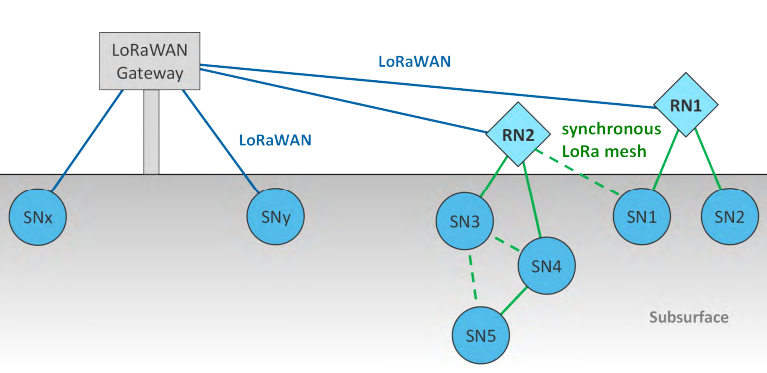
\includegraphics[width=0.6\textwidth]{Figures/synchronouslorameshnetwork.png}
	\caption{Schéma Synchronous LoRa Mesh. Prevzaté z \cite{synchronouslorameshnetwork}}
	\label{fig:synchronouslora}
\end{figure}


\section{Porovnanie a návrh rozšírenia}
Niektoré zo spomenutých riešení využívajú smerovacie tabuľky na efektívnejší prenos dát v rámci siete. Tie môžu byť však limitáciou pokiaľ 
chceme dosiahnuť vyššej mobility uzlov. V prípade, že by sme chceli spolu so smerovacími tabuľkami podporovať mobilitu uzlov, je potrebné zabezpečiť 
dostatočné časté aktualizácie smerovacích tabuliek.

Niektoré spomenuté riešenia limitujú komunikáciu medzi uzlami na vyhradené časové okná, mimo ktoré su uzly v úspornom režime. To môže byť 
veľkou limitáciou pri niektorých aplikáciách, kde je potrebná komunikácia v reálnom čase  (napr. chat).

V tejto práci sme navrhli protokol, ktorý nevyužíval žiadne smerovacie tabuľky. Vďaka tomu bola dosiahnutá vysoká mobilita uzlov. 
Hlavným využitím nášho protokolu bola ad-hoc komunikácia, preto protokol nepoužíval 
žiadnu časovú synchronizáciu a časové okná vyhradené na komunikáciu, uzly siete tak mohli prijímať a odosielať dáta kedykoľvek to bolo potrebné.
To so sebou ale prinášalo nevýhodu v podobe vyššej spotreby energie.

Funkcionalita navrhnutého protokolu, podobne ako niektoré zo spomínaných riešení, fungovala na základe multi hop flooding, 
kedy sa správa v sieti preposielala cez uzly siete až kým nedorazila do destinácie.
Správa sa odoslala a uzol, ktorý túto správu prijal ako posledný ju preposlal ďalej. Toto sa opakovalo na ostatných uzloch v sieti až kým sa správa nedostala do destinácie alebo kym správe nedošiel limit preskokov, prípade TTL.

Navrhnutý protokol nebol závislý na žiadnych špeciálnych centrálnych uzloch typu gateway, prípadne nejakých riadiacich uzloch. Každý uzol v sieti mohol byť jednoduchým uzlom, ktorý prijímal a preposielal dáta ďalej.
Vďaka tomu mohli byť uzly realizované prostredníctvom lacných a malých zariadení.

Protokol bolo možné používať na rôznych platformách. V tejto práci vznikla implementácia protokolu pre mikrokontroléry používajúce programovací jazyk C++ a 
mikrokontroléry alebo jednodoskové počítače podporujúce CircuitPython.

Na šifrovanie obsahu správ bol použitý šifrovací algoritmus AES.


\renewcommand{\thefootnote}{\fnsymbol{footnote}}
\begin{table}[!h]
	\centering
  \small
  \setlength\tabcolsep{3pt}
	\caption[Porovnanie LoRa mesh protokolov]{Porovnanie LoRa mesh protokolov}
  \begin{tabular}{c|c|c|c|c|c|c}
    \toprule
    Protokol  & \makecell{LoRa \\ mesher} & Meshtastic & LoRaBlink & Pymesh & \makecell{Synchronous\\ LoRa Mesh} & Náš protokol\\
    \midrule
    Centrálne uzly & Nie & Nie & Áno & Áno & Áno & Nie \\
    \hline
    Mobilita uzlov & Áno\footnotemark[7] & Áno & Áno\footnotemark[1] & Áno\footnotemark[7] & Áno\footnotemark[1] & Áno\\
    \hline
    Smerovanie & \makecell{Distance \\ Vector} & Flooding & Flooding & \makecell{Distance \\ Vector} & Flooding & Flooding\\
    \hline
    Ad-hoc komunikácia & Áno & Áno & Nie & Áno & Nie & Áno \\
    \midrule
  \end{tabular}
  \label{tab:compar}
\end{table}
\footnotetext[1]{Po zmene polohy mobilného uzla, je potrebné čakať pokým nastane ďalšia epocha}
\footnotetext[7]{Po zmene polohy mobilného uzla, je potrebné nájsť a aktualizovať cestu k nemu v smerovacích tabuľkách}
\renewcommand{\thefootnote}{\arabic{footnote}}

\chapter{Vlastná implementácia}
Ako sme už spomínali v predchádzajúcej kapitole, nami vytvorený protokol fungoval na základe multi hop flooding. Tento prístup so sebou ale niesol 
niekoľko nevýhod, ktoré sme museli zohľadniť pri navrhovaní implementácie.

Jednou z nevýhod bolo, že ak sme poslali niekam správu, a destinácia práve nebola v dosahu, tak sme o správu prišli. Tento problém bol vyriešený tak, 
že odosielateľ si odoslané správy ukladá a v prípade, že sa nepodarí správu doručiť, môže ju opätovne 
odoslať niekedy neskôr. To, že sa správu nepodarilo doručiť do destinácie, sme zisťovali vďaka potvrdzovacím ACK správam. 

Ďalším z problémov mohlo byť potenciálne zahltenie siete správami. Keby každý uzol v sieti preposielal ďalej každú správu, ktorú prijal, tak by sme sa rýchlo dostali 
do stavu kedy by množstvo uzlov preposielalo rovnaké správy a sieť by sa tym pádom zahltila.
Riešenie tohto problému spočívalo v niekoľkých procesoch ako stavu zahltenia predchádzať. Tieto procesy si bližšie popíšeme v kapitole implementácie.

V tejto práci vznikli dve verzie implementácie. Jedna verzia, implementovaná v CircuitPython, bola určená pre výkonnejšie zariadenia. Táto implementácia obsahovala aj webové rozhranie na 
obsluhu, posielanie a prijímanie sprav. Webové rozhranie avšak šlo využiť len na zariadeniach, ktoré podporujú WiFi prípadne ethernet.

Implementácia v C++ bola určená pre menej výkonne zariadenia. Táto implementácia bola len zjednodušená verzia kompletnej implementácie a 
bola primárne určená pre mikrokontroléry TTGO. Z dôvodu výkonnosti a obmedzenej pamäti táto implementácia obsahovala iba základné funkcionality protokolu, potrebné na odosielanie správ s 
údajmi so senzorov. Mikrokontroléry TTGO tak v sieti fungovali iba ako jednoduché uzly, ktoré v určitých časových intervaloch odosielali dáta zo senzorov.

\section{Typy a stavy správ}
Predom sme si stanovili, že v našom protokole bude možné odosielať rôzne typy správ. Na základe typov správ, sa potom správy spracovávajú odlišne.

Okrem typov správ, bolo nutné si definovať aj určité stavy, v ktorých sa správa môže nachádzať. Tieto stavy potom určovali, ako sa správa spracováva.
\subsection{Typy správ}
Rozhodli sme sa v našom protokole implementovať dokopy sedem typov správ. Každý typ správy má svoju úlohu a využitie.
Sú nasledovné:

ACK správa slúžila na potvrdenie doručenia správy. Keď odosielateľ pôvodnej správy niekedy neskôr prijal ACK správu, ktorá 
potvrdzovala doručenie správy, tak mohol pôvodnú správu považovať za doručenú.

Textová správa (TEXT\_MSG) je správa, ktorá obsahovala textový reťazec. Rozšírením tejto správy je správa s potvrdením o doručení (TEXT\_MSG\_W\_ACK).
Obsah textových správ je šifrovaný.

Správa typu senzorové dáta (SENSOR\_DATA) bola určená na prenos dát z rôznych senzorov. Obsah správy bol taktiež vo forme textového 
reťazca, ktorý obsahoval dáta zo senzorov. Tento typ správ avšak oproti obyčajnej textovej správe ponúkal možnosť nastaviť 
časový interval -- TTL, po ktorého uplynutí sa správa nebude ďalej šíriť sieťou. Obsah správy bol taktiež šifrovaný.

Sprava žiadosť o traceroute (TRACEROUTE\_REQUEST) bola používaná len v krajných prípadoch, kedy nás zaujímalo akou cestou sa správa preposiela sieťou. 
Ked nejaký uzol prijal správu typu žiadosť o traceroute, tak vytvoril novu správu typu odpoveď na traceroute (TRACEROUTE) a vložil do nej svoju adresu. 
Adresátom tejto novej správy bol odosielateľ pôvodnej správy. Ked sa táto odpoveď na traceroute šírila sieťou, 
tak každý uzol, ktorý danú správu preposlal ďalej, pridal do nej svoju vlastnú adresu.
Takto sa vytvoril reťazec, ktorý obsahoval adresy všetkých uzlov, cez ktoré bola správa preposlaná.
Aby mohli ostatné uzly v sieti do správy postupne pridávať svoje adresy, tak obsah tejto správy nemohol byť šifrovaný.

Posledným typom správy je nespracovaný paket (RAW\_PACKET). Tento typ správy bol využívaný iba v prípade, že ma používateľ zapnutý monitorovací režim.
V tomto režime sa zaznamenávali všetky správy, ktoré sa v sieti prenášali. V tomto režime bolo možne zachytiť aj pakety, 
ktoré neboli súčasťou nášho protokolu a ich štruktúra nezodpovedala našim špecifikáciám. Z toho dôvodu ich nebolo možné spracovať a 
uložili sa teda ako typ správy nespracovaný paket. Ich obsah tvorili iba holé prijaté dáta vo forme bajtov.

\subsection{Stavy správ}
Na správnu funkčnosť bolo potrebné aby správy existovali v určitých stavoch. Správy časom svoj stav aktualizovali a prechádzali medzi nimi. 
Tieto stavy boli definované nasledovne:

Stav nová správa (NEW). Tento stav bol určený pre správu, ktorá bola práve vytvorená. Nebola ešte ani raz odoslaná aktuálnym uzlom, a čaká na svoje 
prvé odoslanie. Po prvom odoslaní sa správa presunula do stavu odoslaná (SENT).

Zo stavu odoslaná bolo možne správu presunúť do stavu neúspešná (FAILED), hotová (DONE), preposlaná (REBROADCASTED) alebo zmazaná (DELETED). 
Ak aktuálny uzol prijal tu istú správu, odoslanú iným uzlom, znamená to, že dana správa sa šíri ďalej v sieti. Aktuálny uzol teda správu 
presunul do stavu preposlaná alebo do stavu zmazaná. 
To či sa správa presunula do stavu zmazaná alebo preposlaná bolo závisle od toho, či bol aktuálny uzol zároveň aj autorom danej správy. V prípade, že bol autorom, 
správa sa presunula do stavu preposlaná.

Správy v stave preposlaná, pri ktorých nepotrebujeme sledovať, či správa dorazila do destinácie, sa následne presunuli do stavu hotová.

Pokiaľ aktuálny uzol vyčerpal všetky pokusy o odoslanie správy, prípadne pri správe typu senzorové dáta došiel časový limit, správa sa presunula do stavu neúspešná alebo zmazaná.
To či sa presunula do stavu neúspešná alebo zmazaná bolo znovu závisle na tom, či bol aktuálny uzol autorom danej správy alebo nie.

Správam, ktoré boli v stave preposlané sa odpočítaval časový limit na prijatie potvrdenia. Pokiaľ v tomto časovom intervale nedorazila potvrdzovacia ACK správa, tak sa 
správa presunula do stavu nepotvrdená (NAK). V opačnom prípade sa presunula do stavu potvrdená (ACK).

Stav zmazaná značil, že správu považujeme za vymazanú. Ďalej s ňou už nebudeme pracovať a po uplynutí určitého intervalu sa reálne vymazala z pamäti.

Zjednodušený diagram prechodu medzi jednotlivými stavmi správ je vyobrazený na obrázku v prílohe \ref{fig:stateDiagram}.

\section{Návrh paketu}
Paket obsahoval hlavičku a dátový rámec. Štruktúra dátového rámcu bola závislá od typu správy.
Navrhnutú štruktúru hlavičky paketu môžme vidieť v tabuľke \ref{tab:packetHeader}

\begin{table}[!h]
	\centering
  \caption{Štruktúra hlavičky paketu a dĺžka jednotlivých polí v bajtoch.}
  \begin{tabular}{|c|c|c|c|c|c|c|}
    \toprule
    2B uint & 2B uint & 4B uint & 2B uint & 1B uint & 1B uint & 0 -- 240B \\
    \midrule
    Destinácia & Odosielateľ & ID správy & Kontrolný súčet & Typ správy & Priorita & Dátový rámec \\
    \midrule
  \end{tabular}
  \label{tab:packetHeader}
\end{table}

Pre adresy odosielateľa a destinácie boli využité dvoj bajtové adresy. Pre broadcast adresu bola rezervovaná hodnota 0xFFFF. 
Štvor bajtový identifikátor správy bol náhodne generovaný pri každom vytvorení novej správy.

Z adresy destinácie, adresy odosielateľa a identifikátoru správy bol vytvorený dvoj bajtový kontrolný súčet. Tento kontrolný súčet bol používaný na overenie, či prijatá správa 
patrila do nášho protokolu. Overovať integritu dát na základe kontrolného súčtu nie je za potreby, pretože táto kontrola je už zahrnutá na fyzickej vrstve LoRa technológie.

Položka typ správy obsahovala číslo, ktoré definovalo typ danej správy. Číslo reprezentovalo jeden z typov spomínaných v predošlej sekcii.

Správam bolo možné v hlavičke paketu určiť vyššiu prioritu. Na túto prioritu sa následne bral ohľad pri spracovávaní správ a správy s vyššou prioritou boli odbavené prioritne. 
Rozhodli sme sa poskytovať iba dva stupne priority správ a to normálna priorita a vysoká priorita. 

Dátové rámce sa líšili na základe typu správy. V tabuľkách \ref{tab:textFrame}, \ref{tab:trFrames} a \ref{tab:frames} 
sú uvedené štruktúry dátových rámcov pre jednotlivé typy správ.


\begin{table}[!h]
	\centering
  \caption{Štruktúra dátového rámcu pre textové správy.}
  \begin{tabular}{|c|c|c|}
    \toprule
    1B uint & 1B uint & 0 -- 238B String \\
    \midrule
    Počet skokov & Pôvodný počet skokov & Textové dáta \\
    \midrule
  \end{tabular}
  \label{tab:textFrame}
\end{table}

\begin{table}[h!]
  \centering
  \subfloat[\centering Správa typu žiadosť o traceroute.]{{
    \begin{tabular}{|c|c|}
      \toprule
      1B uint & 1B uint \\
      \midrule
      Počet skokov & Pôvodný počet skokov \\
      \midrule
    \end{tabular}
  }}
  \qquad
  \subfloat[\centering Správa typu odpoveď na traceroute.]{{
    \begin{tabular}{|c|c|}
      \toprule
      1B uint & 0 -- 239B String\\
      \midrule
      Počet skokov & Navštívené adresy \\
      \midrule
    \end{tabular}
  }}
  \caption{Štruktúra dátového rámcu pre správy typu traceroute.}
  \label{tab:trFrames}
\end{table}

V niektorých dátových rámcoch môžme vidieť položku počet skokov. Do tejto položky bol pri vytvorení novej správy zapísaný maximálny počet skokov, ktoré môže správa vykonať 
pri prenose sieťou. Každý uzol, predtým ako správu preposlal ďalej, zmenšil počet skokov o jedna. Ak sa počet skokov dostal na nulu tak sa daná správa ďalej nespracovávala a nastavil sa jej 
adekvátny stav.

V rámcoch tiež nájdeme položku pôvodný počet skokov. Do tejto položky bol tak isto pri vytvorení novej správy zapísaný maximálny počet skokov. Hodnota v tejto položke sa 
však už ďalej nemenila. Slúžila k tomu, aby prijímateľ dokázal zistiť, koľko preskokov správe zabralo, kym správa dorazila až k nemu. Túto informáciu bolo možné 
následne použiť na správne nastavenie maximálneho počtu skokov pre odoslanie potvrdzovacej správy, prípadne správy typu odpoveď na traceroute.

\begin{table}[h!]
  \centering
  \subfloat[\centering Potvrdzovacie ACK správy.]{{
    \begin{tabular}{|c|c|}
      \toprule
      1B uint & 4B uint \\
      \midrule
      Počet skokov & ID potvrdzovanej správy \\
      \midrule
    \end{tabular}
  }}
  \qquad
  \subfloat[\centering Správy pre senzorové dáta.]{{
    \begin{tabular}{|c|c|}
      \toprule
      2B uint & 0 -- 238B String \\
      \midrule
      TTL & Senzorové dáta \\
      \midrule
    \end{tabular}
  }}
  \caption{Štruktúra dátového rámcu pre ACK a senzorové správy.}
  \label{tab:frames}
\end{table}

V dátovom rámci, používanom na senzorové dáta, bol použitý, namiesto maximálneho počtu preskokov, TTL. TTL vyjadruje časový interval, po ktorý mohla byť daná správa 
spracovávaná a preposielaná v sieti. Táto hodnota sa pri vytvorení správy nastavila na predom určený časový interval v sekundách. Každý uzol, ktorý danú správu preposielal, 
si overil ako dlho už bola správa uložená u neho v pamäti a na základe toho odčítal hodnotu z TTL. Po odčítaní hodnoty z TTL, uzol správu ďalej preposlal.

Pri odčítavaní TTL bol braný do úvahy iba čas, ktorý daná správa strávila na určitom uzle. Nebral sa do úvahy čas, ktorý správe zabralo preniesť sa rádiovými vlnami z jedného uzlu 
na ďalší. A to z toho dôvodu, že sme neboli schopní presne určiť, aku vzdialenosť prekonala vysielaná správa rádiovými vlnami. Existujúce spôsoby merania vzdialenosti, 
ktorú správa prešla vzduchom, produkovali len hrubé odhady a boli veľmi závisle od aktuálnych atmosférických podmienok. Preto sme sa rozhodli, že v našom riešení budeme 
počítať iba s časom, ktorý správa strávila na určitom uzle. Mimo toho, keby sme počítali s maximálnou možnou vzdialenosťou medzi dvoma uzlami, ktorá sa pri LoRa 
udáva okolo 15 kilometrov v otvorenom priestranstve, a rýchlosťou ktorou sa šíria rádiové vlny, ktorá je vo vákuu rovná rýchlosti svetla, tak by sme zistili, 
že prenos správy medzi týmito dvoma uzlami by v ideálnom prípade trval okolo 50 mikrosekúnd. Táto hodnota bola v porovnaní s časom, ktorý správa strávi na určitom uzle, 
zanedbateľná.

\section{Funkcionalita protokolu}
Navrhnutý protokol fungoval tak, že každý uzol si u seba uložil novo prijatú správu. Následne boli uložené správy spracovávané v hlavnom cykle programu. 
Každú správu, ktorú uzol prijal, sa následne pokúšal znovu preposlať ďalej, pokiaľ teda nebola daná správa určená práve tomu uzlu.

Uzol každú správu odosielal iba určitý počet krát a medzi každým odoslaním konkrétnej správy uzol čakal predom stanovený časový interval predtým ako ju mohol znova odoslať.
Toto viacnásobne odosielanie každej správy nám zabezpečilo vyššiu spoľahlivosť v doručení. Keby sa každá správa preposielala iba jeden krát, mohlo by sa stať, že na ten prvý raz 
by tuto vyslanú správu nezachytil žiaden ďalší uzol a správa by sa tak nedoručila ďalej.

Medzi tým ako boli správy spracovávané a preposielané, uzol zároveň počúval na novo príchodzie správy od iných uzlov. Ak náhodou uzol 
prijal správu, ktorá už bola prijatá a uložená u neho tak to považoval ako potvrdenie, že sa správa šírila ďalej v sieti. Uzol teda u seba danú správu zahodil a už ju 
ďalej nepreposielal.

Ak došlo k situácií, kedy uzol jednu správu opakovane preposlal maximálny možný počet pokusov a medzitým neprijal danú správu preposlanú iným uzlom, 
tak bola považovaná táto situácia ako neúspešne odoslanie správy. Správe sa nastavil adekvátny stav a nebola ďalej spracovávaná.

Každý uzol prijatej správe znížil hodnotu maximálneho počtu preskokov. Pokiaľ sa však jednalo o správy typu senzorové dáta, tak sa neznižovala hodnota maximálneho počtu preskokov 
ale hodnota TTL, a to pred každým znovu odoslaním danej správy. Pokiaľ však uzol prijal správu, ktorej hodnota maximálneho počtu skokov dosiahla nulu, tak táto 
správa nebola u daného uzla ani ukladaná. Ak sa počas spracovávania správ na uzle dostala hodnota TTL nejakej senzorovej správy na nulu, tak táto situácia bola tak isto považovaná 
za neúspešne odoslanie správy. Správe sa nastavil adekvátny stav a nebola ďalej spracovávaná.

Obsah textových a senzorových správ bol vždy šifrovaný, pokiaľ nebola správa posielaná na broadcast adresu. Na šifrovanie bol použitý šifrovací algoritmus AES, ktorý šifruje bloky dát za pomoci kľúča.
Jedna sa o symetrickú šifru, takže zašifrované dáta bolo možné rovnakým kľúčom neskôr dešifrovať. To ponúkalo možnosť aby si určitá skupina používateľov vytvorila vlastný 
šifrovací kľúč a iba oni boli schopní dešifrovať svoje správy, ktoré boli vytvorené za použitia tohto kľúča. Ostatní účastníci siete obsah správ neboli schopní dešifrovať.

V protokole bolo možné odosielať správy aj na broadcast adresu. Tieto správy boli potom prijaté každým uzlom.

\section{Implementácia protokolu}
Hlavnou súčasťou nami navrhnutého protokolu bol zoznam správ. Do tohto zoznamu boli pridávané novo vytvorené, 
prípadne novo prijaté správy. Následne bol tento zoznam správ v hlavnom cykle programu prechádzaný a každá správa sa bola spracovávaná.

Na to aby bolo možné správy do tohoto zoznamu ukladať, bolo potrebné vytvoriť istú dátovú štruktúru, do ktorej by sa ukladali jednotlivé správy.
Správy v zozname so sebou držali rôzne informácie. Okrem tých základných informácií o správe akými boli napríklad jej identifikátor, odosielateľ a prijímateľ, obsah správy atď., 
bolo potrebné držať spolu so správou aj dodatočné informácie, ktoré boli potrebné na jej následne spracovávanie. Do týchto dodatočných informácií patrili napríklad 
čas, kedy bola správa naposledy spracovávaná aktuálnym uzlom. Táto informácia bola využitá pri kontrole či uz nadišiel čas správu znovu preposlať ale aj 
na to aby bolo možné zistiť koľko času treba odčítať z hodnoty TTL pri senzorových správach.

Pri prechádzaní zoznamu správ sa pri každej správe skontroloval jej stav a to či časový limit už dosiahol požadovanej hodnoty. Opakované znovu odosielanie 
správy, bolo vykonávané iba pri správach v stave nová a odoslaná. Spomínali sme, že je bolo možne určiť správe vyššiu prioritu. Tato vyššia priorita zabezpečila to, že sa pri správe, 
ktorá má nastavenú vyššiu prioritu, vykonávalo opakované znovu odosielanie správy, aj keď jej časový limit ešte nebol dosiahnutý. Tým bolo dosiahnuté toho, že správa sa 
skôr odoslala a do destinácie by mala v ideálnom prípade doraziť skôr ako správa s nižšou prioritou.

Spomínali sme tiež, že môže dôjsť k problému zahltenia siete, keby každý uzol v sieti preposielal všetky správy, ktoré príjme. Spôsob akým sme vzniku tohto problému zabránili 
spočíval práve v tom, že keď uzol prijal správu, ktorú už mal u seba uloženú, tak u seba tuto správu označil ako zmazanú ( stav zmazaná ) a správa nebola ďalej preposielaná. 
Správy v zmazanom stave neboli ale ihneď vymazané z pamäti. Miesto toho sa im nastavoval časový interval a až po tom čo uplynul tento interval boli správy skutočne vymazané z pamäti. 
Vďaka tomu, že sme si držali v pamäti správy aj keď boli považované za zmazané, bolo možné overiť či novo prijatá správa nebola náhodou jedná z tých zmazaných. Ak áno tak nová 
správ nebola znovu ukladaná. K tejto situácii môže bežne dochádzať a neošetrenie tohto problému by mohlo viesť k zacykleniu, kedy by sa jedna a ta istá správa neustále 
preposielala medzi dvoma uzlami až kým by jej nedošiel limit skokov prípadne TTL.

Aby bolo v mesh sieti dosiahnuté čo najlepšieho dosahu, bolo nutné nejak zabezpečiť, aby sa odosielané správy dostali k čo najvzdialenejším uzlom a aby tieto 
najvzdialenejšie uzly boli tie ktoré propagujú prenášanú správu ďalej. To bolo zabezpečene tak, že každej novo prijatej správe bolo nastavené prvotné časové oneskorenie na základe 
toho s akou hodnotou SNR bola daná správa prijatá. Hodnota SNR vyjadruje pomer signálu k šumu. Čím je hodnota SNR vyššia, tým je signál silnejší oproti okolitému šumu.
Vďaka tomu, bolo možné približne odhadnúť, ktorý uzol bol vzdialenejší. Uzly ktoré boli vzdialenejšie mali nižšiu hodnotu SNR a teda aj nižšiu hodnotu časového oneskorenia.
To poviedlo k tomu, že vzdialenejšie uzly odvysielali správu skôr, ako uzly ktoré boli bližšie. Ostatné uzly toto vysielanie prijali, a u seba označili danú správu ako zmazanú, 
keďže už nebolo potrebné aby ju oni preposielali.

Ďalší z potrebných aspektov správneho fungovania nášho protokolu bolo zabezpečiť aby nedošlo k situácií kedy by dva alebo viac uzlov v sieti začalo vysielať signály v rovnakom čase.
K tomu bol využitý takzvaný prístup listen before talk, kedy sa uzol predtým ako začal vysielať presvedčil, či náhodou práve nevysielal niekto iný v jeho dosahu. Ak áno tak tak sa vyslanie správy pozdržalo 
a skúsilo sa odoslať neskôr.

Rozhodli sme sa implementáciu protokolu začať na zariadeniach Armachat. Keďže sme zatiaľ nemali vytvorené žiadne užívateľské rozhranie, tak veľké farebné displeje na zariadeniach Armachat 
boli vhodné na zobrazovanie informácií o prebiehajúcich procesoch a komunikácií v sieti. Na programovanie zariadení Armachat bol použitý CircuitPython, ktorý ma ale rovnakú syntax ako 
programovací jazyk Python.

Ako prvé bolo potrebné vytvoriť vhodnú dátovú štruktúru, ktorá by uchovávala v sebe správu. K tomu bola vytvorená trieda Message. Trieda obsahovala všetky potrebné informácie o správe. 
Taktiež obsahovala metódy na vytváranie rôznych typov a obsahov správ. Tieto metódy slúžili na prvotné vytvorenie nových správ, na autorskom uzle. Okrem týchto metód bolo 
ale potrebné mať aj metódy, ktoré dokázali z prijatých dát vytvoriť správu. Pri prijatí nového paketu v LoRa, sme dostali dáta vo forme bajtového poľa. Tieto dáta boli potom predané 
do metódy, ktorá z nich vytvorila správu.

Po implementácií triedy Message, sme teda boli schopní vytvoriť novu správu alebo prijať bajtové pole z LoRa, z ktorého sa následne poskladala správa. Na to aby sme 
mohli správy ukladať do zoznamu správ bolo ale potrebné vytvoriť ešte akýsi kontajner, ktorý by v sebe uchovával správu plus dodatočne informácie potrebne k ďalšiemu spracovávaniu.
K tomu vznikla trieda MessageQueueItem. Tá v sebe držala inštanciu triedy Message, počítadlo opakovaných odoslaní, časový odpočet, časové razítko, ktoré zachytávalo čas, kedy bola 
správa naposledy spracovávaná, aktuálny stav správy a ďalšie užitočné informácie. Okrem toho obsahovala táto trieda metódy, ktoré boli využívane pri spracovávaní správ. Sem patria metódy na zníženie maximálneho počtu preskokov alebo 
TTL, metóda na zmenu stavu správy, metóda na aktualizovanie časového razítka, ktorá časové razítko nastavila na aktuálny čas a mnoho ďalších.

Po implementácii triedy MessageQueueItem sme mohli začať implementovať samotný proces funkcionality nášho protokolu. Zoznam správ bol realizovaný ako slovník, 
kde kľúčom bol identifikátor správy, a hodnota pod daným kľúčom bola inštanciou triedy MessageQueueItem. To nám umožnilo rýchlo vyhľadávať správy na základe jej identifikátora. 
Tento slovník sme pomenovali message queue a tak ku nemu budeme referovať aj vo zvyšku tejto práce.

Hlavný proces protokolu pozostával z cyklu, v ktorom bolo najskôr skontrolované či náhodou nebol prijatý nový LoRa paket a následne boli prejdené všetky správy z message queue. Ak to bolo 
potrebné tak sa určité správy spracovali. K tomu vznikli dve hlavné funkcie. Funkcia receive(), ktorá slúžila na skontrolovanie či nebol prijatý nový LoRa paket a funkcia tick(), v ktorej boli prejdené všetky správy z message queue.

Funkcia receive() prečítala novo prijatý paket z LoRa a následne overila, či daný paket spĺňa dĺžku aspoň 12 bajtov. Vychádza to z toho, že všetky správy nášho protokolu obsahujú predom definovanú 
hlavičku paketu (viď. Tab. \ref{tab:packetHeader} ), ktorá mala veľkosť 12 bajtov. Ak bol paket kratší ako 12 bajtov, bolo možné s istotou povedať, že sa nejednalo o správu nášho protokolu a teda ho nebolo 
nutné ďalej spracovávať. Po kontrole dĺžky paketu, nasledovalo overenie kontrolného súčtu. Funkcia zobrala prvých 8 bajtov paketu a vypočítal sa z nich kontrolný súčet. 
Ak sa vypočítaný kontrolný súčet zhodoval s kontrolným súčtom, ktorý bol v pakete, tak bolo možné správu považovať za 
súčasť nášho protokolu. Na výpočet kontrolného súčtu bola použitá funkcia cyklicky redundantného súčtu typu CRC-16/CCITT-FALSE. Overovanie, či paket prisluhuje do nášho protokolu bolo pomerné dôležité, 
pretože na rovnakých LoRa parametroch mohli byť vysielané aj pakety iných protokolov a tieto pakety by sa nam nepodarilo správne spracovať keďže by nespĺňali našu štruktúru paketu.

Potom čo sa vo funkcii receive() overilo, že paket spĺňa naše požiadavky, bola z neho vytvorená nova inštancia triedy Message. Bola k tomu využitá metóda triedy Message určená na vytvorenie správy z 
poľa bajtov. Pri novo prijatej správe nás zaujímalo či je správa určená nám. Ak bola správa určená nám, bolo potrebné zistiť o aky typ správy sa jednalo. Pokiaľ bola prijatá správa typu ACK, tak bolo 
nutné vyhľadať v message queue korešpondujúcu správu a zmeniť jej stav na ACK. Pokiaľ sa nejednalo o ACK správu, nasledovala kontrola, či sa daná správa už nenachádzala v message queue a ak nie tak tam bola pridaná.

Bolo dôležité, aby uzol po prijatí správy, odoslal naspäť ACK správu. A to aj v prípade, že sa nejednalo o typ správy, ktorý vyžadoval potvrdenie o doručení. Dôvodom bolo to, že ak by 
uzol neposlal naspäť ACK správu, tak by predošlý uzol pokračoval v opakovanom vysielaní správy, a tieto vysielania by zbytočne obsadzovali prenos v sieti. Uzol teda po prijatí vyslal ACK správu. 
V prípade, že prijatá správa nevyžadovala potvrdenie o doručení, tak mohol uzol ACK správe nastaviť maximálny počet preskokov na 0. 
Tým pádom sa správa neposunula ďalej v sieti ako k najbližšiemu uzlu. Ak sa ale jednalo o správu vyžadujúcu potvrdenie o doručení, tak sa maximálny počet preskokov nastavil na 
hodnotu, ktorá bola uložená v prijatej správe pod položkou pôvodný počet skokov. 
Tym bolo zaručené, že správa bude mať dostatočný počet dostupných skokov aby sa dostala naspäť k uzlu, ktorý pôvodnú správu poslal.

V prípadnom scenári, že prijatá správa nebola určená nám, bolo skontrolované či sa rovnaká správa už nenachádzala v message queue a ak nie tak tam bola pridaná za predpokladu, že mala ešte dostupný 
nejaký počet skokov alebo TTL. Správe bolo zároveň nastavené prvotné časové pozdržanie na základe hodnoty SNR, s ktorou bola prijatá.

V opačnom prípade, kedy sa sprava už nachádzala v message queue, bolo nutné znova vykonať sériu overení a na základe nich zmeniť stav správy.
Prvé z overení bolo, či daná správa bola vytvorená nami. To či bola vytvorená nami, sme zistili na základe toho, či sa adresa odosielateľa správy zhodovala s tou našou. 
V tom prípade nastala situácia kedy našu správu preposlal nejaký iny uzol. Bolo možné teda správe zmeniť stav na hotovo, prípadne na stav preposlaná ak sa jednalo o správu s potrebným 
potvrdením o doručení.

Ak sa ukázalo, že správa nebola vytvorená nami ale niekým iným, tak bola správa presunutá do stavu zmazaná. Do tohto stavu bola ale presunutá iba v prípade overenia, že hodnota počtu preskokov alebo TTL 
z prijatej správy bola nižšia ako hodnota správy v message queue. %TODO tu mozno vysvetlit preco sa to tak robi

Po dokončení funkcie receive(), nasledovala funkcia tick(). V tejto funkcii bolo postupne prechádzane všetkými spravami z message queue. Pri každej správe bol overený jej stav 
a ak bola v stave preposlaná alebo zmazaná tak sa následne skontrolovalo, či jej už nevypršal časový limit. Pokiaľ limit vypršal, tak sa správa 
skutočne vymazala z message queue ak bola v stave zmazaná. Ak bola v stave preposlaná, tak sa jej stav zmenil na nepotvrdená -- NAK.

V prípade, že bol stav správy nová alebo odoslaná, tak sa pokračovalo v jej spracovávaní, ktoré pozostávalo z následujúcich krokov.
Ako prvé bolo overené, či už nadišiel čas danú správu spracovať. To bolo zistené tak, že sme sa pozreli či správe už vypršal časový limit. Ak áno, znamenalo to, že správa bola pripravená na spracovávanie 
a bolo možné pokračovať ďalej. Ak nie tak sa daná správa preskočila a prešlo sa na ďalšiu správu.

Ak nadišiel čas správu spracovať, tak bolo skontrolované, či má ešte dostupné nejaké pokusy o odoslanie a v prípade senzorových správ aj to, či bol ešte dostupný TTL.
Ak došlo k situácii, že správa už vyčerpala všetky pokusy o odoslanie alebo jej TTL došlo na nulu, tak bola správa presunutá do stavu neúspešná alebo zmazaná ak to nebola 
správa vytvorená nami. Ak správe ešte zostali nejaké pokusy o odoslanie, tak bola správa odoslaná cez LoRa. Keď sa jednalo o správu typu senzorové dáta, tak sa správe pred 
odoslaním zmenšila hodnota TTL.

Po odoslaní bolo správe aktualizované aktuálne časové razítko, znížilo sa počítadlo dostupných pokusov o odoslanie a bol nastavený nový časový limit pre správu. Tento 
limit bol závislý od konfiguračnej premennej, ktorá určovala, ako často sa ma správa znovu odosielať. Pokiaľ bola správa pred odoslaním v stave nová, tak jej stav bol aktualizovaný 
na odoslaná.

Pri pokuse o odoslanie mohlo dôjsť k situácií, kedy práve niekto iný vysielal signál a tak bolo nutné pozdržanie odoslania. To bolo realizované tak, že správe bolo nastavené 
časové pozdržanie na hodnotu konfiguračnej premennej a bolo aktualizované jej časové razítko. Výsledkom bolo, že táto správa sa pokúšala znovu odoslať až po uplynutí 
časového intervalu.

Po dokončení implementácie hlavnej funkcionality sme ju mohli otestovať. Na zariadeniach Armachat sme vytvorili jednoduché rozhranie, 
ktoré zobrazovalo na displeji informácie o novo prijatej správe. Taktiež bolo možné využiť klávesnicu zariadenia, na napísanie vlastnej správy a jej odoslanie.
Na obrázku \ref{fig:armRec} môžme vidieť, že zariadenie prijalo správu od odosielateľa s adresou 0xA1BC, ktoré bolo v tomto prípade druhé Armachat zariadenie.
\begin{figure}
	\centering
	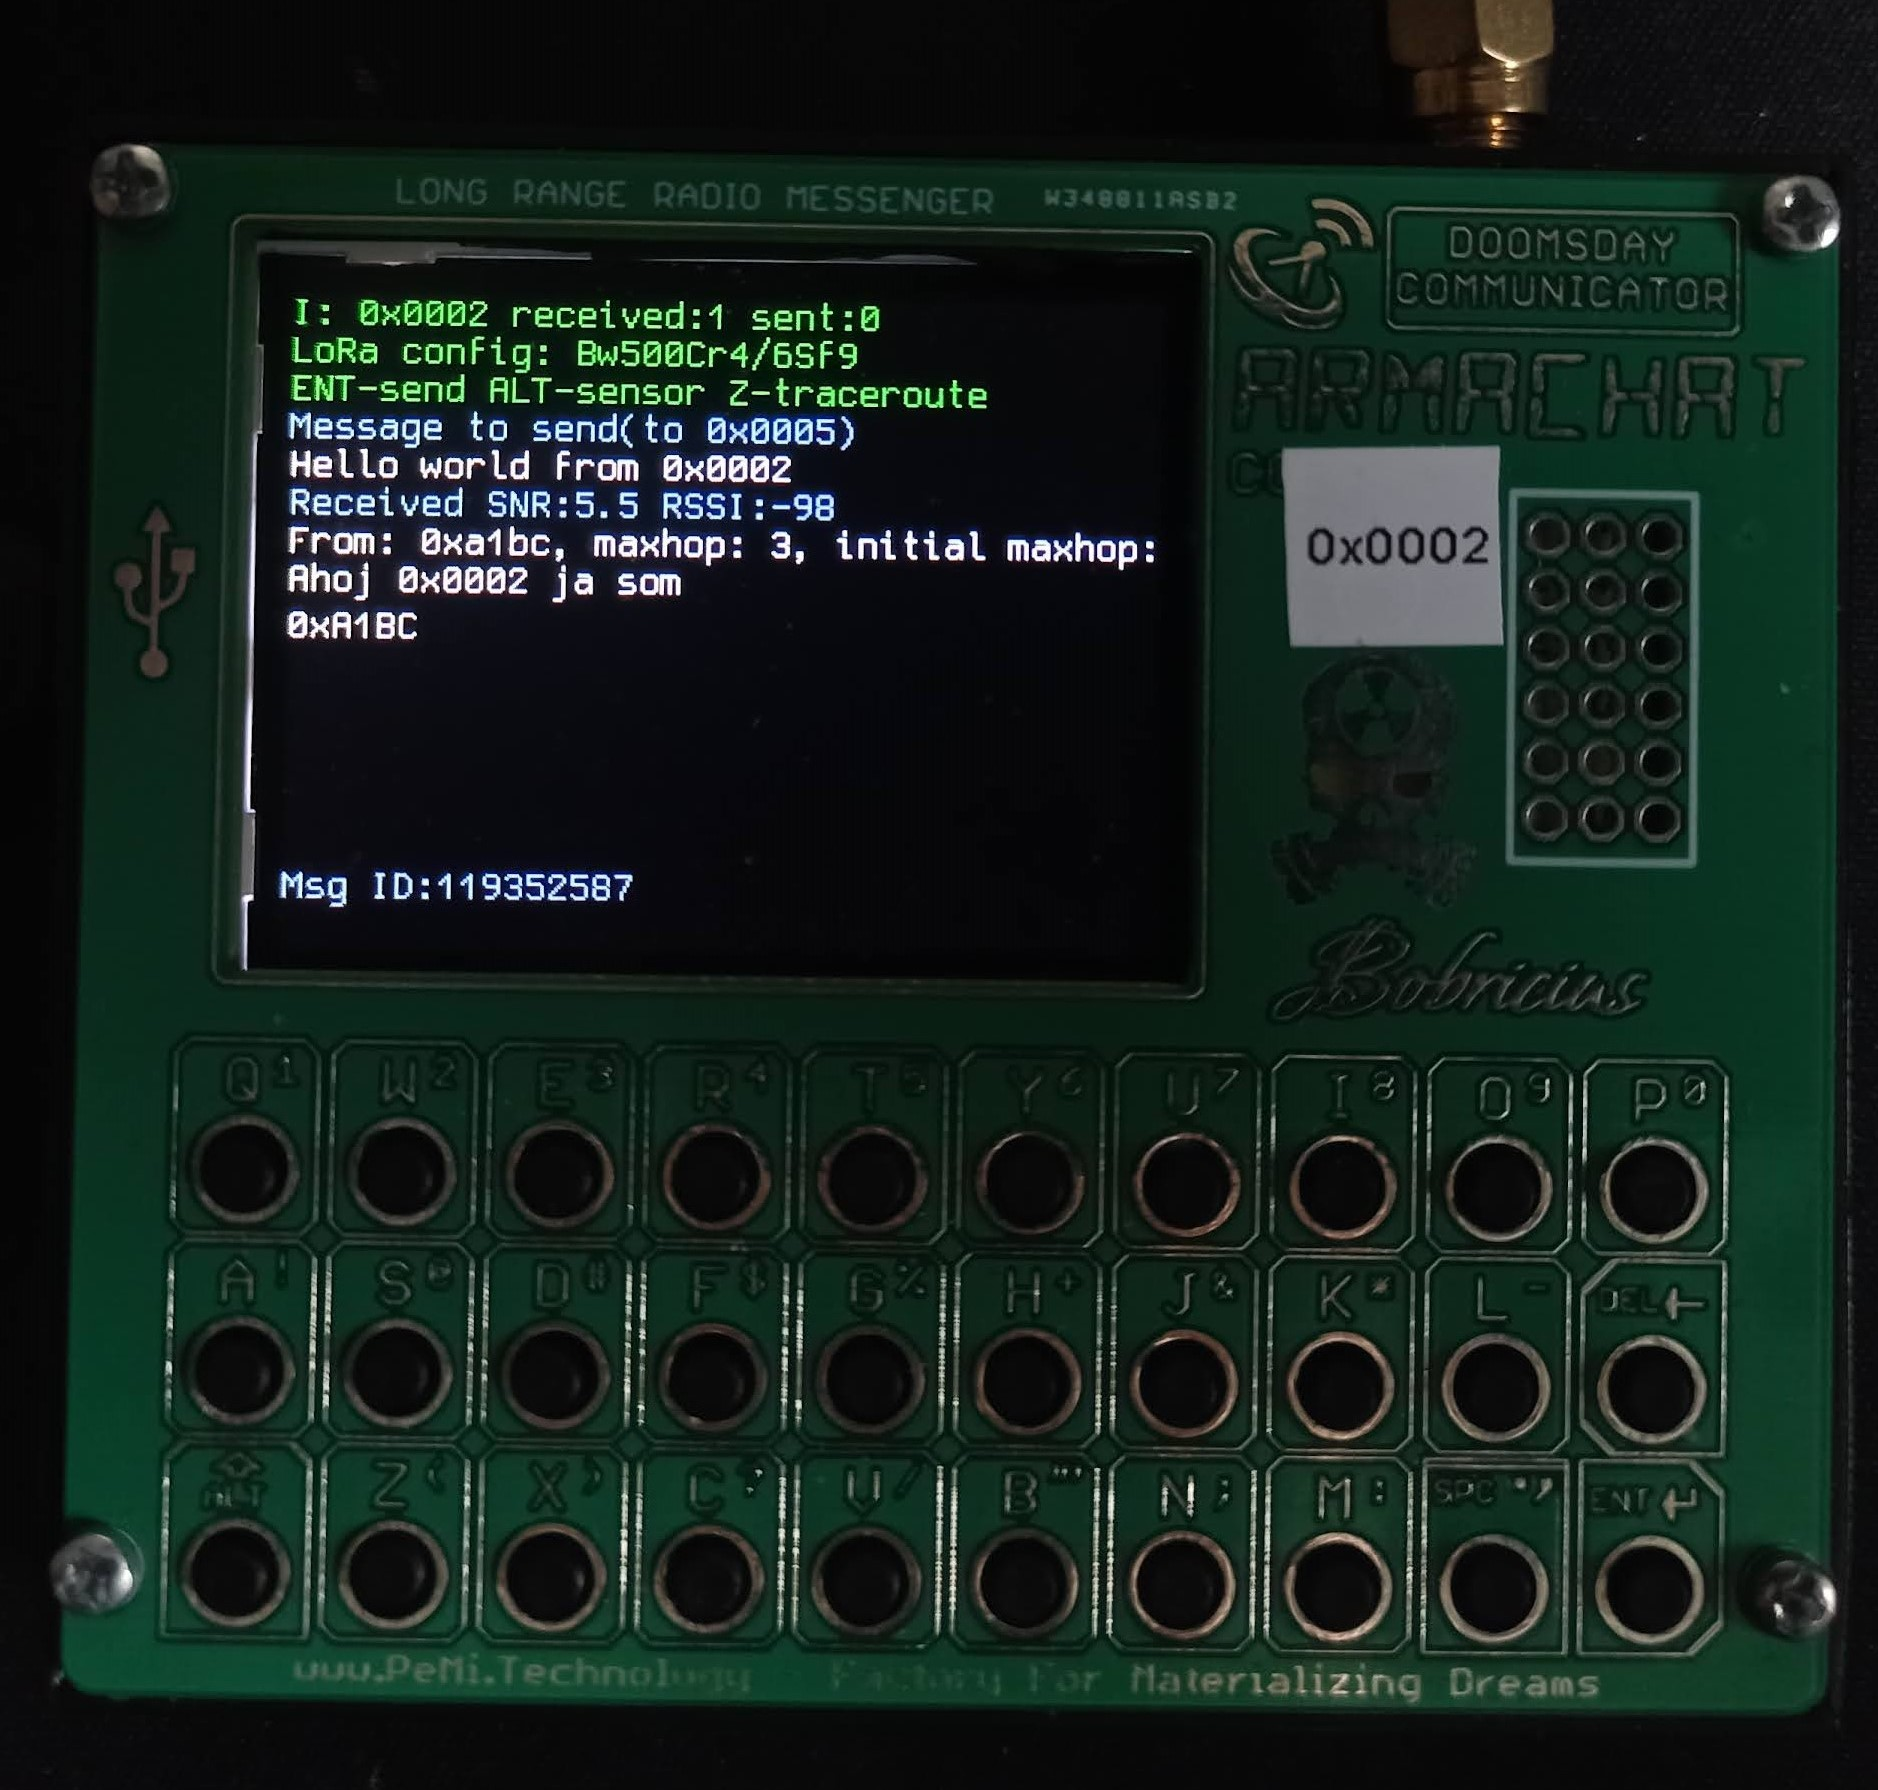
\includegraphics[width=0.6\textwidth]{Figures/armRec.jpg}
	\caption{Rozhranie zariadenia Armachat}
	\label{fig:armRec}
\end{figure}

Okrem obsahu správy, môžme vidieť hodnoty SNR a RSSI, s ktorými zariadenie správu prijalo, hodnotu max hop, ktorá predstavovala počet preskokov a hodnotu initial max hop, 
ktorá predstavovala pôvodný maximálny počet preskokov. Na základe rovnosti týchto dvoch hodnôt, môžme usúdiť, že správa prešla medzi dvoma zariadeniami bez toho aby prešla 
cez nejaké iné tretie zariadenie. Na spodku displeja môžme vidieť identifikátor prijatej správy.

Na ďalšom obrázku \ref{fig:armRec2} môžme vidieť, že rozdiel medzi hodnotami max hop a initial max hop bol 1. Indikuje to, že správa spravila preskok cez ďalšie zariadenie predtým ako 
bola doručená na cieľové zariadenie. Tento test sme vykonali tak, že sme tri zariadenia rozmiestnili s určitou vzdialenosťou medzi nimi, tak aby sme docielili preskok cez jedno zariadenie. 
Zariadenia mali nastavené adresy 0x0001, 0x0002 a 0xA1BC. Správa bola odoslaná zo zariadenia 0xA1BC na zariadenie 0x0002.

Taktiež si môžme všimnúť zmenu v podobe skrátenia názvov atribútov max hop a initial max hop, z dôvodu, že sa na displeji nezmestili do jedného riadku.
Okrem toho je na obrázku vidieť informačnú správu v podobe žltého textu na samom spodku displeja. V tejto informačnej správe sa zobrazujú 
rôzne informačné hlášky počas behu programu. Zariadenie 0x0002 prijalo správu od zariadenia 0xA1BC a následne vytvorilo ACK správu, ktorej ID bolo 1787352650.
V informačnej správe môžme vidieť, že v dobe vyhotovenia fotografie sa akurát táto ACK správa pridávala do message queue.

\begin{figure}
	\centering
	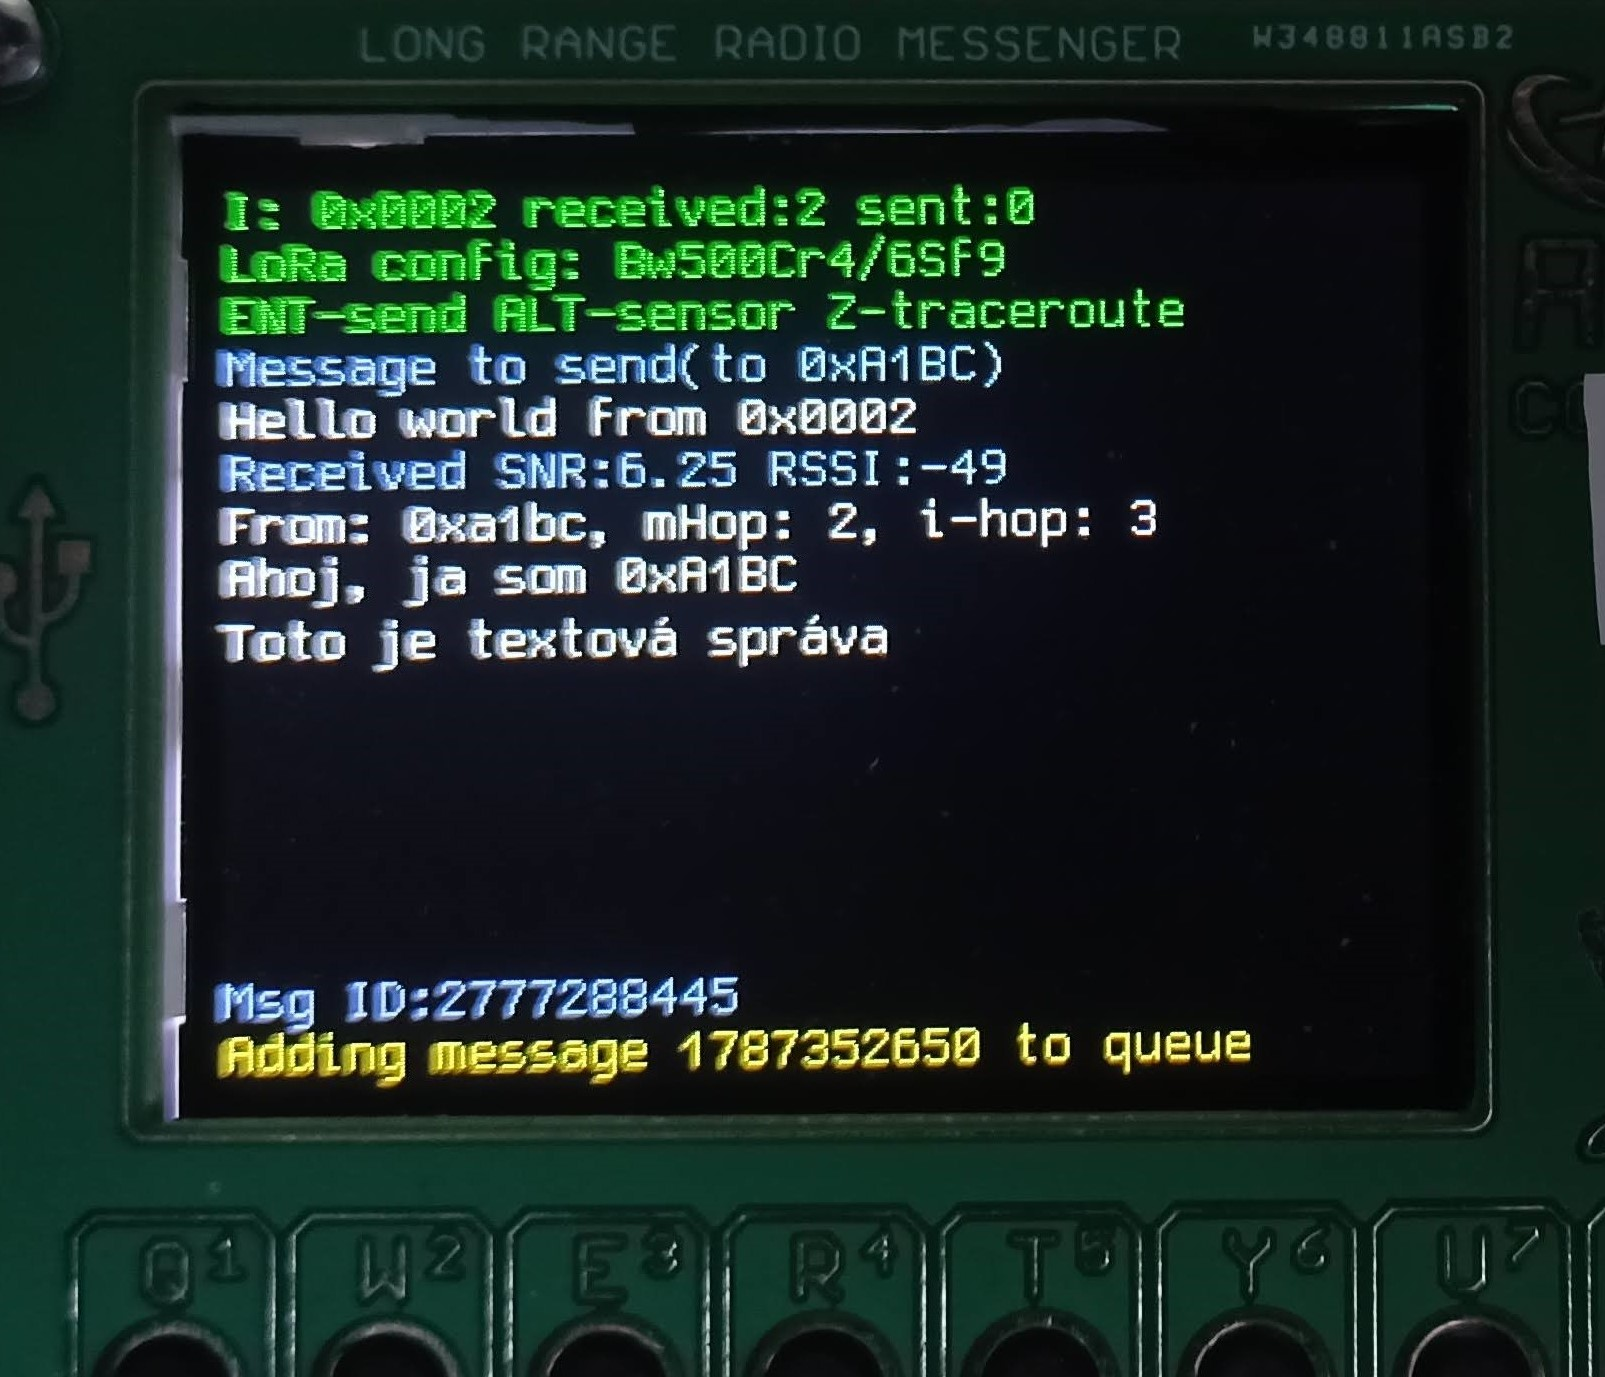
\includegraphics[width=0.6\textwidth]{Figures/armRec2.jpg}
	\caption{Zariadenie Armachat prijalo spravu s jedným preskokom}
	\label{fig:armRec2}
\end{figure}

Následne sme vyskúšali, pri rovnakom rozmiestnení zariadení, odoslať zo zariadenia 0x0002 žiadosť o traceroute na zariadenie 0xA1BC. Na obrázku \ref{fig:armTraceroute} môžme 
vidieť, ako zariadenie 0x0002 prijalo odpoveď na žiadosť o traceroute. V obsahu správy vidíme zoznam adries, cez ktoré správa putovala.

V tabuľke \ref{tab:packet} môžme vidieť vygenerovaný paket vo forme bajtov, ktorý bol odoslaný zo zariadenia 0xA1BC na zariadenie 0x0002. Obsah správy bol v tomto prípade, 
textový reťazec \uv{Ahoj}. V prvých 12 bajtoch, vidíme hlavičku paketu. V ďalších 6 vidíme počet preskokov, pôvodný počet preskokov a šifrovaný obsah správy.

\begin{figure}[!h]
	\centering
	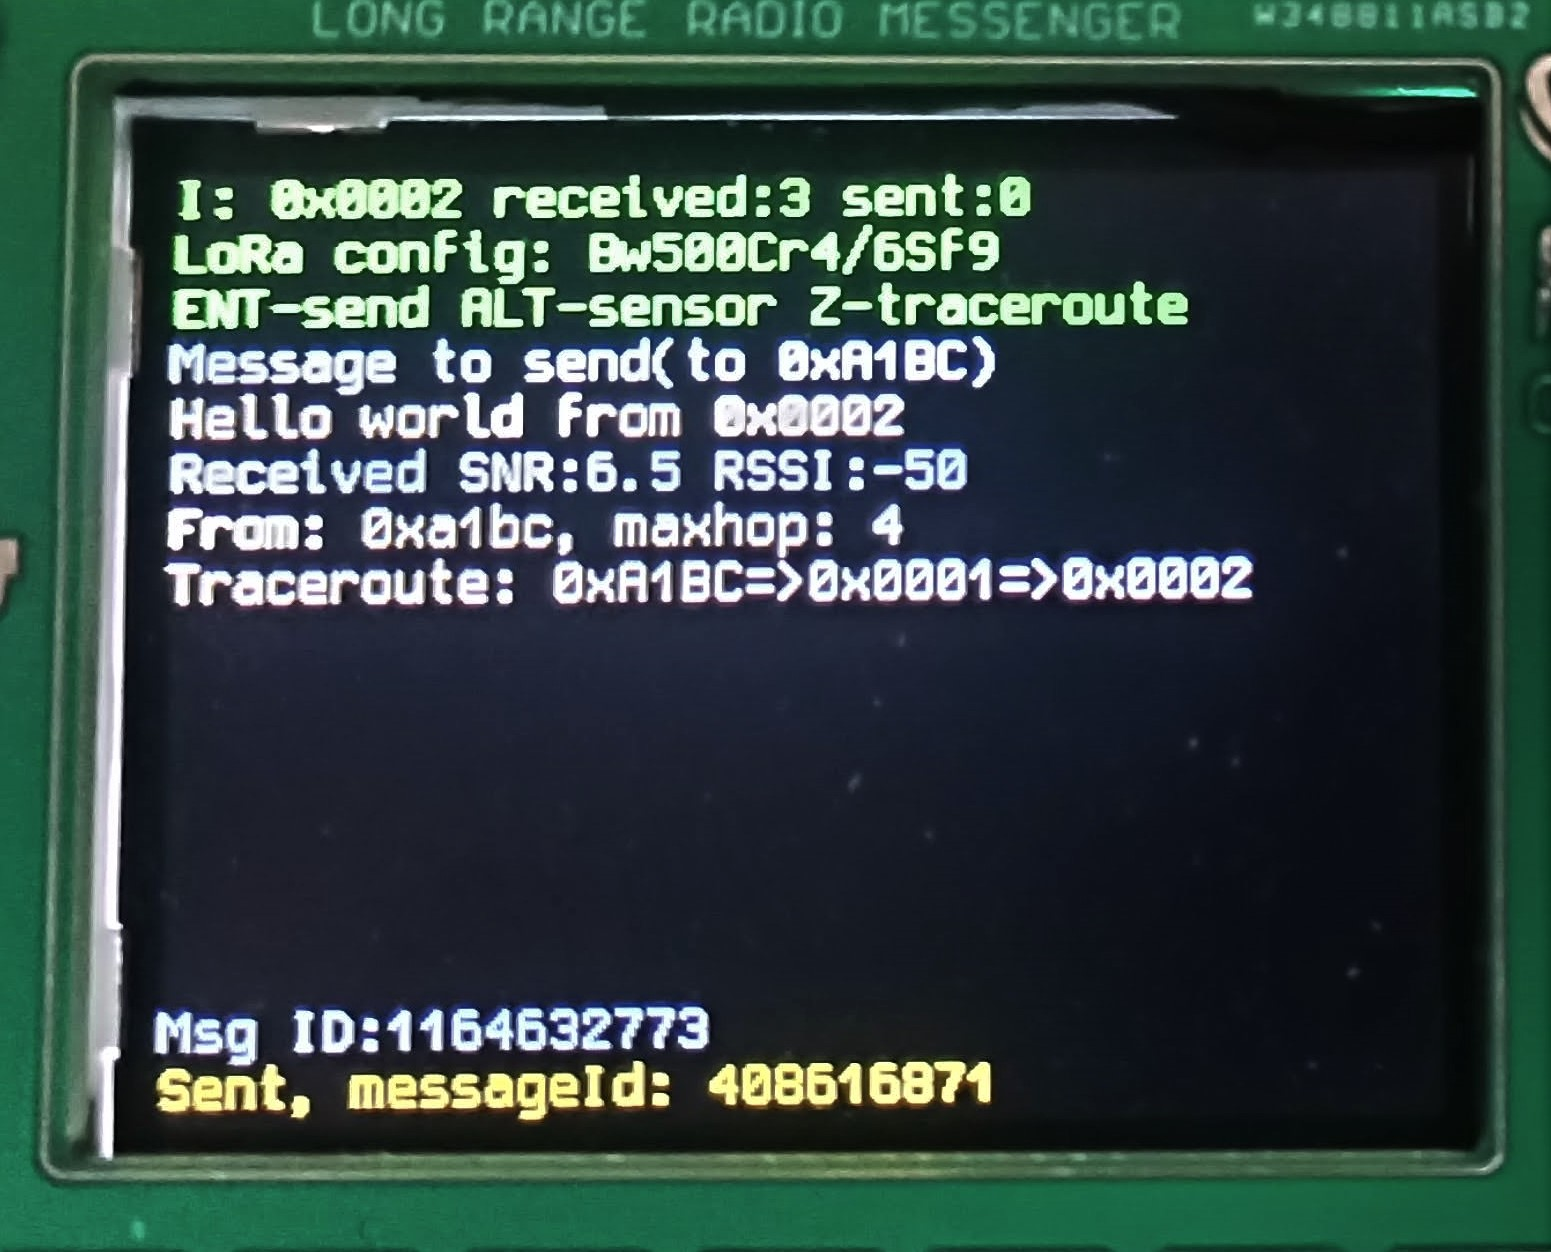
\includegraphics[width=0.7\textwidth]{Figures/armTraceroute.jpg}
	\caption{Zariadenie Armachat prijalo traceroute správu}
	\label{fig:armTraceroute}
\end{figure}

\begin{table}[!h]
  \small
  \setlength\tabcolsep{2pt}
	\centering
  \caption{Ukážka bajtov odoslaného paketu}
  \begin{tabular}{ c c | c c | c c c c |c c |c | c || c | c | c c c c }
    \multicolumn{12}{c ||}{Hlavička} & \multicolumn{6}{c}{Dátový rámec} \\
    \midrule
    0x00 & 0x02 & 0xA1 & 0xBC & 0xEF & 0x42 & 0x5D & 0xC2 & 0xF2 & 0x64 & 0x01 & 0x00 & 0x02 & 0x03 & 0xA4 & 0x4A & 0x33 & 0x56 \\
    \midrule
    \multicolumn{2}{c |}{\rotatebox[origin=c]{ 90}{Destinácia}} & \multicolumn{2}{c |}{\rotatebox[origin=c]{ 90}{Odosielateľ}} &
    \multicolumn{4}{c |}{ID správy} & \multicolumn{2}{c |}{\rotatebox[origin=c]{ 90}{Kontrólny súčet}} &
    \multicolumn{1}{c |}{\rotatebox[origin=c]{ 90}{Typ správy}} & \multicolumn{1}{c ||}{\rotatebox[origin=c]{ 90}{Priorita správy}} &
    \multicolumn{1}{c|}{\rotatebox[origin=c]{ 90}{Max hop}} & \multicolumn{1}{c|}{\rotatebox[origin=c]{ 90}{Initial max hop}} & \multicolumn{4}{c}{Šifrovaný obsah správy}\\
  \end{tabular}
  \label{tab:packet}
\end{table}

\section{Implementácia API pre webové rozhranie}
Pri používaní nášho protokolu mal používateľ možnosť využiť webové rozhranie, cez ktoré bolo možné ovládať zariadenie a 
pracovať s naším LoRa protokolom. Používateľ mal možnosť vytvárať alebo prijímať nove správy, ktoré sa zobrazovali na webovej stránke.
Okrem toho bolo možné cez webové rozhranie konfigurovať rôzne nastavenia týkajúce sa nášho protokolu, ako napríklad adresu zariadenia 
alebo nastavenie LoRa parametrov.

K tomu aby bolo možné cez webové rozhranie ovládať zariadenie a protokol, bolo nutné najskôr implementovať nejaké API. 
Cez API sme mohli komunikovať so zariadením z webového rozhrania. Toto API bežalo na serveri, ktorý bol spustený na zariadení 
spolu s naším protokolom. API bolo realizované prostredníctvom klasických HTTP požiadavkov.

Najpodstatnejšími časťami API boli funkcie, ktoré nám umožnili prijímať alebo odosielať správy. K tomu vznikli dve 
API prístupové body -- takzvané routy. \uv{/api/messages} a \uv{/api/send text message}.

Prvá routa slúžila na získanie správ, ktoré boli prijaté na zariadení. Bola volaná prostredníctvom HTTP GET požiadavku a 
vraciala zoznam obsahujúci entity jednotlivých správ. Každá správa bola reprezentovaná JSON objektom, ktorý obsahoval 
iba potrebné informácie o správe, k tomu aby bolo možné zobrazovať správy na webovej stránke. Štruktúru tohoto JSON 
objektu môžme vidieť na ukážke \ref{fig:messageObj}.

\begin{figure}[h!]
	\centering
	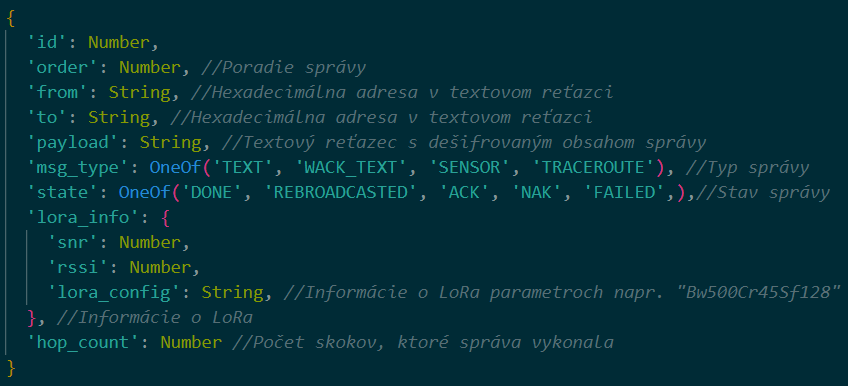
\includegraphics[width=0.9\textwidth]{Figures/msgObject.png}
	\caption{Štruktúra JSON objektu reprezentujúceho správu}
	\label{fig:messageObj}
\end{figure}

Druhá routa slúžila na odosielanie správ prostredníctvom HTTP POST požiadavku. Táto routa prijímala JSON objekt, ktorý reprezentoval novú správu.
V JSON objekte musia byť uvedené všetky potrebné informácie o správe, ktoré sú potrebné na jej správne odoslanie. 
Boli nimi destinácia, maximálny počet skokov, priorita, obsah správy a príznak, či chceme potvrdenie o doručení. 
API po prijatí požiadavku na vytvorenie novej správy validovala vstupné údaje a ak boli všetky údaje v poriadku, tak bola vytvorená nová správa. V 
opačnom prípade API vrátila chybovú hlášku. Z dôvodu limitácie LoRa paketov na maximálnu dĺžku 255 bajtov pre posielané dáta, bolo potrebné overiť či textová správa 
nie je príliš dlhá a prípadne ju orezať na maximálnu povolenú dĺžku.

Maximálna povolená dĺžka v tomto prípade nie je 255 bajtov ale len 238. Toto je výsledkom toho, 
že použitá LoRa knižnica povoľuje maximálnu dĺžku paketu 252 bajtov a to kvôli kompatibilite s inými knižnicami.
Pri našom protokole je okrem toho v každom LoRa pakete potrebné nejaké miesto ešte rezervovať pre hlavičku paketu a informácie o počte skokov.
Z toho nám ostáva maximálna dĺžka správy 238 bajtov.

Ďalším potrebným API prístupovým bodom bola routa na získavanie a zmenu aktuálnej konfigurácie. 
Vznikla na to routa \uv{/api/config}. Táto routa mohla byť volaná prostredníctvom HTTP GET požiadavku, kedy vrátila aktuálnu konfiguráciu 
alebo prostredníctvom HTTP PUT požiadavku, kedy nastavila novú konfiguráciu z poskytnutého JSON objektu, zachytávajúceho nové nastavenia.

Používateľ má možnosť nastaviť rôzne parametre, ktoré ovplyvňujú správanie protokolu. Nastavené hodnoty parametrov boli ukladané do 
JSON súboru na zariadení, konkrétne na umiestnení /data/settings.json. Tieto nastavenia si bližšie popíšeme v časti implementácie 
konfiguračného rozhrania.

\section{Návrh webového rozhrania}
Pred samotnou implementáciou webového rozhrania bolo nutné vytvoriť nejaký návrh, 
ako bude webové rozhranie vyzerať. Na vytvorenie návrhov webových stránok bol použitý dizajnérsky nástroj Figma \cite{figma}.

Bolo potrebné navrhnúť dokopy štyri web stránky, kde prvou bola úvodná stránka na ktorej mohol používateľ vidieť prijaté a odoslané správy. 
Taktiež tam bola možnosť odoslať novú správu.

Rozhodli sme sa pridať aj možnosť ukladať si kontakty do adresára, ktorý umožňoval používateľovi vidieť namiesto 
hexadecimálnych adries v správach, názov uloženého kontaktu. Tieto kontaktné adresáre boli rozdelené pre kontakty na iných používateľov a kontakty 
ne senzorové uzly. Z toho dôvodu boli potrebné dve ďalšie stránky, kde by používateľ mohol spravovať svoje kontakty.

Poslednou stránkou bola stránka na konfiguračné rozhranie. Táto stránka obsahovala všetky možnosti, ktoré mal používateľ možnosť nastavovať.

Výsledne návrhy môžeme vidieť na následujúcich obrázkoch. Stránky pre správu kontaktov ( Obr. \ref{fig:figma2} ) na používateľov a kontaktov na senzorové uzly budú vyzerať 
rovnako.

Na obrázku \ref{fig:figmaHome} zachytávajúcom návrh úvodnej stránky si môžme všimnúť, že niektoré adresy sú zobrazené ako mená z kontaktov.

Pri tvorbe návrhu stránky na konfiguráciu nastavení ( Obr. \ref{fig:figma2} ), nebolo ešte známe, aké všetky nastavenia 
bude môcť používateľ meniť a tak sú tam iba nastavenia adresy, šifrovacieho kľúča a LoRa parametrov.

\begin{figure}[h!]
  \centering
  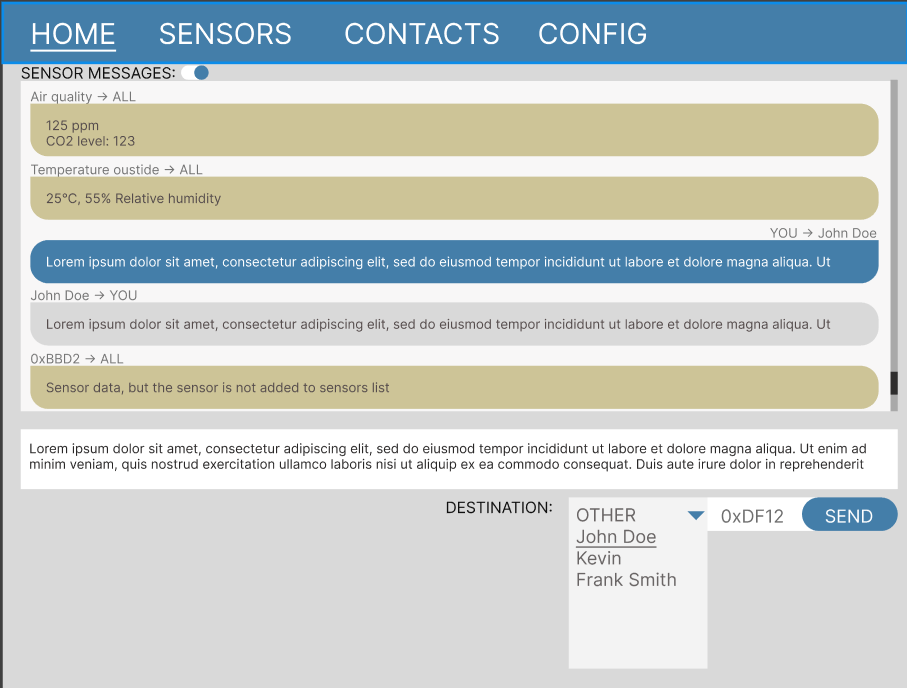
\includegraphics[width=0.9\textwidth]{Figures/figmaHome.png}
  \caption{Návrh úvodnej stránky}
  \label{fig:figmaHome}
\end{figure}

Keďže bola pridaná novú funkciu v podobe pridávania kontaktov, bolo potrebné vytvoriť novú API routu, ktorá vraciala 
zoznam kontaktov. Okrem toho bola vytvorená ďalšia routa, slúžiaca na pridávanie nových alebo mazanie starých kontaktov. 
Ako databáza kontaktov bol použitý JSON súbor, do ktorého sa kontakty ukladali priamo na zariadení do súborov /data/contacts.json a /data/sensors.json. 

\begin{figure}[h!]
  \centering
  \subfloat[\centering Kontakty]{{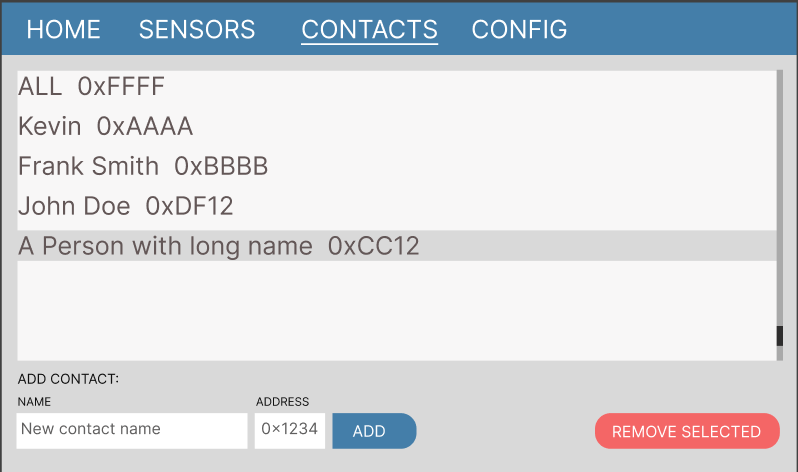
\includegraphics[width=0.77\textwidth]{Figures/figmaContacts.png} }}
  \qquad
  \subfloat[\centering Nastavenia]{{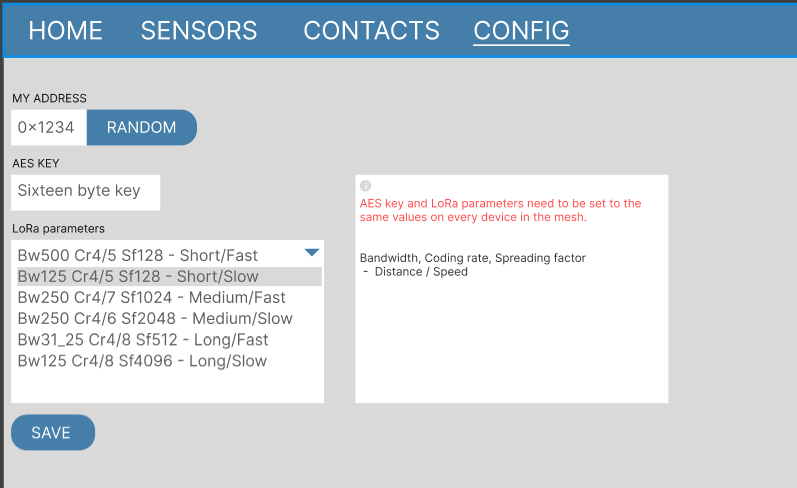
\includegraphics[width=0.76\textwidth]{Figures/figmaSettings.png} }}
  \caption{Návrhy stránok kontaktov a nastavení}
  \label{fig:figma2}
\end{figure}

\section{Implementácia webového rozhrania}
Na implementáciu webového rozhrania bola použitá kombinácia HTML, CSS a JavaScriptu. Na komunikáciu s API bolo použité fetch API, 
ktoré je súčasťou JavaScriptu. Ukážku volania za použitia fetch API môžeme vidieť v nasledujúcom kóde.
\newpage
\begin{lstlisting}[language=Python, label={lst:fetch}]
  const newMessage = {
    "destination":"0xA1F4",
    "message":"Ahoj",
    "max_hop":"3",
    "priority":"0",
    "wack":false
  };
  const requestOptions = {
    method: 'POST',
    headers: { 'Content-Type': 'application/json' },
    body: JSON.stringify(newMessage)
  };
  fetch('/api/send_text_message', requestOptions)
\end{lstlisting}

Webové stránky sme implementovali podľa pripravených návrhov. Avšak pri implementácii sme sa rozhodli, že 
niektoré veci trochu pozmeníme a pridáme. Ukážku finálnej implementácie webového rozhrania bude možné vidieť v časti testovania.

Jednou z hlavných zmien bolo pridanie statusu, ku jednotlivým správam. 
Tento status vo forme ikonky bol zobrazovaný pri nami odoslaných správach a indikoval, či bola správa prijatá alebo nie. 
Na obrázku \ref{fig:messageStates} vidíme ukážku, ako tieto jednotlive stavy vyzerali. Môžme si tiež všimnúť, že nad správu 
pribudla dodatočná informácia o použitých LoRa parametroch. Taktiež môžme vidieť nove tlačítko, ktoré sa zobrazovalo pri 
neúspešných správach.

\begin{figure}[h!]
  \centering
  \subfloat{{
    \subfloat[\centering Správa bez potvrdenia o doručení]{{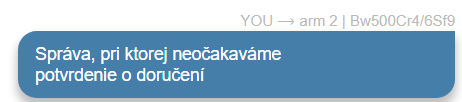
\includegraphics[width=0.4\textwidth]{Figures/nonWackMsg.png} }}
    \subfloat[\centering Správa čakajúca na potvrdenie o doručení]{{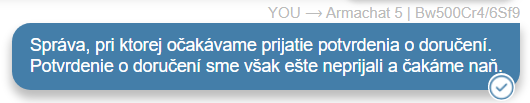
\includegraphics[width=0.4\textwidth]{Figures/ackWaiting.png} }}
  }}
  \newline
  \subfloat{{
    \subfloat[\centering Správa prijala potvrdenie o doručení]{{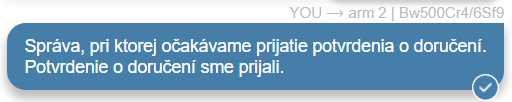
\includegraphics[width=0.45\textwidth]{Figures/ackDone.png} }}
    \subfloat[\centering Správa neprijala potvrdenie o doručení]{{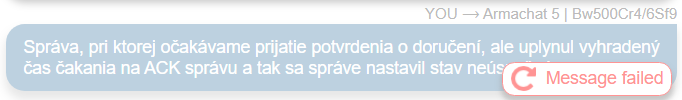
\includegraphics[width=0.5\textwidth]{Figures/ackFailed.png} }}
  }}
  \caption{Informačná ikonka v pravom dolnom rohu pri správach}
  \label{fig:messageStates}
\end{figure}

Tlačítko, zobrazujúce sa pri neúspešných správach, pridalo možnosť neúspešnú správu skúsiť znovu odoslať. K tomu aby to fungovalo, 
bolo potrebné pridať ďalšiu API routu. Táto routa prijímala ako parameter ID správy, ktorú sme chceli odoslať znovu a správa sa znova odoslala.

Stránku nastavení sme voči návrhu rozšírili o ďalšie nastavenia a spolu s tym sme rozšírili aj popis jednotlivých nastavení a čo robia. 
Pri niektorých nastaveniach bolo nutne reštartovať zariadenie, k týmto pribudol popis s informáciou o nutnom reštarte. 
Nastavenia vlastnej adresy bolo obmedzené na jednorázové nastavenie. Týmto sme sa snažili zamedziť tomu, aby si používateľ kedykoľvek 
upravoval svoju adresu a tým sa mohol vydávať za iného používateľa. Finálnu stránku nastavení vidíme na obrázku \ref{fig:webConfig}.

Všetky nastaviteľné položky boli validované predtým, ako sa novo upravené nastavenia odoslali na server. Táto validácia bola potom redundantne 
vykonávaná aj na strane serveru.

Na stránku nastavení sme pridali možnosť pridávať alebo odstraňovať WiFi siete. Na tieto siete sa zariadenie snažilo pripojiť pri spustení a 
po úspešnom pripojení sa spustil webový server. Pribudla aj možnosť definovať si vlastnú sieť typu access point. Pri použití tejto možnosti sa zariadenie pri spúštaní 
nepokúšalo pripájať na žiadnu WiFi sieť, ale vytvorilo svoju vlastnú.

\begin{figure}[h!]
  \centering
  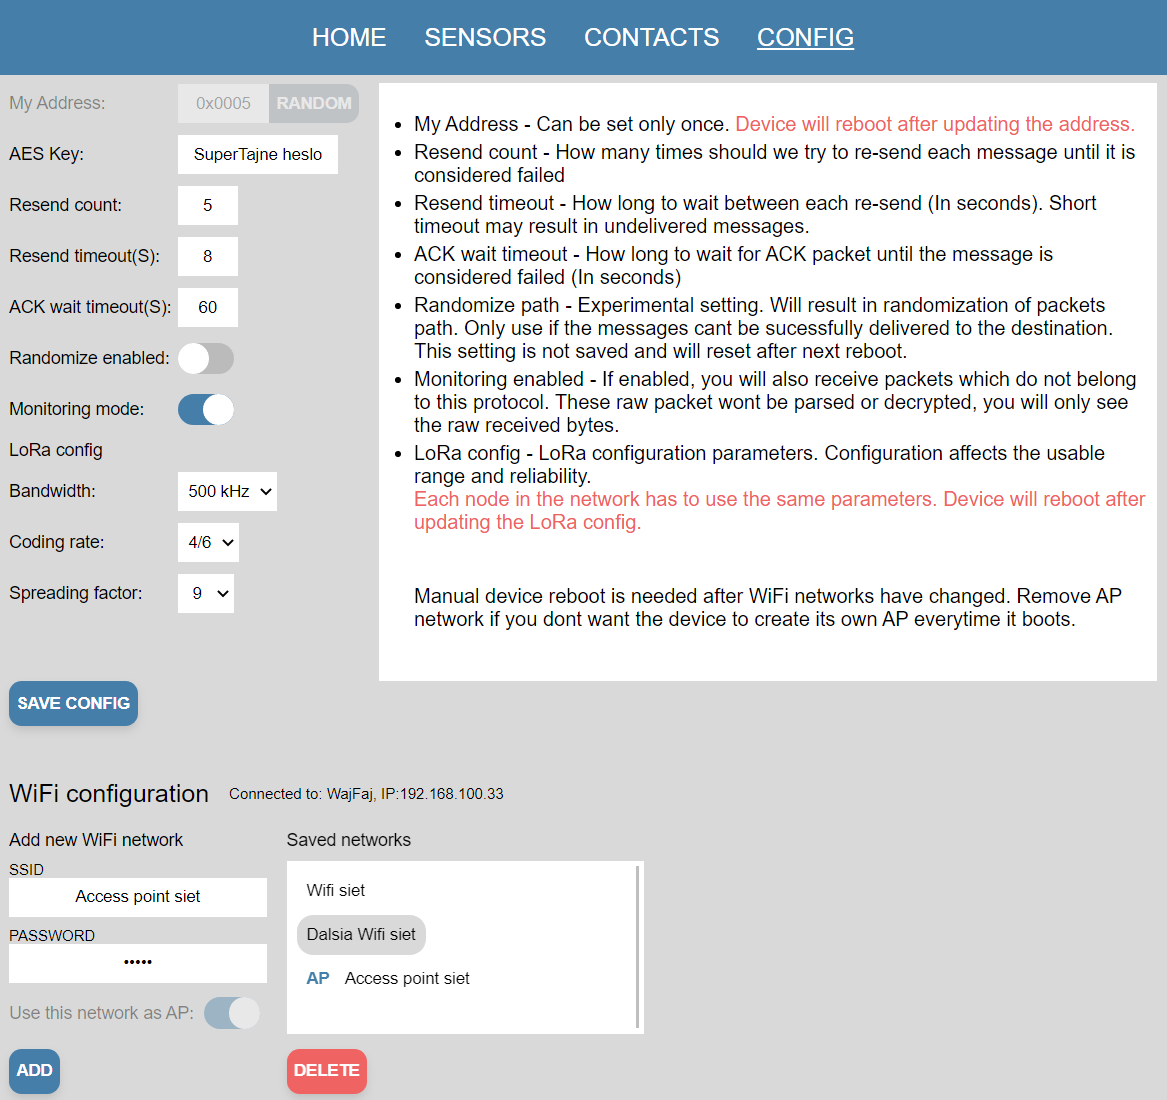
\includegraphics[width=0.9\textwidth]{Figures/webConfig.png}
  \caption{Stránka nastavení}
  \label{fig:webConfig}
\end{figure}
\newpage
\begin{wrapfigure}{r}{0.5\textwidth}
  \begin{center}
    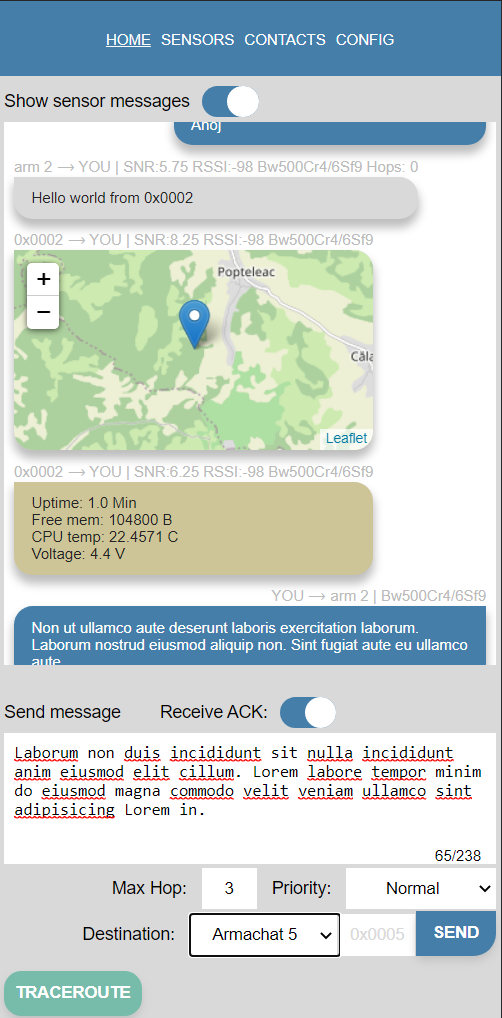
\includegraphics[width=0.5\textwidth]{Figures/mobileWeb.png}
  \end{center}
  \caption{Stránka na mobilnom zariadení}
  \label{fig:mobileWeb}
\end{wrapfigure}

V našej LoRa mesh sieti sa mohli vyskytovať senzorové uzly, ktoré obsahovali GPS modul. Z toho dôvodu sme pridali do webového rozhrania funkciu, 
ktorá zobrazovala na mape aktuálnu polohu zariadenia. Správy, ktoré sme chceli zobraziť ako polohu na mape, museli dodržiavať určitý formát 
a to taký, že správa musela obsahovať prefix \uv{GPS:} a následne nasledovali súradnice zemepisnej šírky a zemepisnej dĺžky oddelene čiarkou.
Ako takáto správa s mapou vyzerala, môžme vidieť na obrázku \ref{fig:mobileWeb}. Na integráciu mapy do webového rozhrania bola použitá knižnica Leaflet.js \cite{leaflet}.

Pri implementácií bol kladený dôraz na to, aby bolo možné webové rozhranie plnohodnotne používať aj na mobilných zariadeniach s malými displejmi. Preto sme 
spravili webové rozhranie responzívne na veľkosť obrazovky. Okrem toho, že sa pri menšej veľkosti obrazovky zmenšovali veľkosti jednotlivých prvkov a písma v rozhraní, 
menilo sa aj celkové usporiadanie prvkov na stránke tak, aby bolo používanie rozhrania prívetivejšie. 

Aby boli odlíšené nami odoslané správy od správ, ktoré sme prijali od nejakého iného uzlu, bolo pridané farebné označenie jednotlivých správ. Správy, ktoré sme 
prijali od iného používateľa boli zobrazené v sivej farbe. Správy ktoré sme prijali od senzorových uzlov, boli zobrazené v žltej farbe. A správy, ktoré sme odoslali 
my, boli modré. Toto farebné označenie je vidieť na obrázku \ref{fig:mobileWeb}. Spomínali sme aj možnosť posielania traceroute správ. Tieto správy boli zobrazené v zelenej farbe.

\section{Optimalizácia}
Po sfunkčnení celej aplikácie sme narazil na problém, v podobe nepostačujúceho miesta na zariadeniach. Dochádzalo k tomu, že ak zariadenie prijalo 
väčšie množstvo správ, tak mu došla pamäť a beh programu sa ukončil.

V zoznam správ boli uložené všetky správy, ktoré boli určené danému uzlu, alebo ktoré sám uzol vytvoril a odoslal. Tento prístup bol však neefektívny, a časom ako 
uzol prijímal a odosielal nove správy, veľkosť zoznamu správ rástla a volná pamäť zariadenia sa postupne znižovala.

Preto sme sa rozhodli, že dĺžku zoznamu správ budeme limitovať. Ak zoznam správ dosiahol určeného limitu, tak sa z neho odstránila najposlednejšia správa.
Po tejto úprave už nedochádzalo k spomínanému problému.

Ďalším problémom, ku ktorému dochádzalo taktiež z nedostatku pamäti bolo, že pri volaní API na získanie správ zariadeniu došla pamäť a program sa ukončil.
Dochádzalo k tomu preto, že funkcia na získanie správ sa snažila celý zoznam správ transformovať do JSON formátu, ktorý by následne poslala nazad. Pri tejto transformácií 
na JSON, sa však všetky dáta z jednotlivých správ kopírovali do nového JSON objektu. Keďže bolo v zozname správ veľa položiek, tak ich kopírovanie do JSON objektu zabralo 
nadmerné množstvo pamäti a program spadol.

API na získanie správ sme preto upravili tak, že používa takzvané stránkovanie. Toto stránkovanie funguje tak, že na API bol zoznam správ rozdelený na menšie časti -- stránky a 
vraciala sa vždy iba jedna stránka. Pri volaní API bol pridaný parameter špecifikujúci, ktorú stránku má API vrátiť. Tento prístup mal za následok, že 
webová stránka volala API na získanie správ nie raz, ale viac krát, až kym nezískala všetky stránky.

Vďaka tejto optimalizácií už nedochádzalo k problému s pamäťou.

\section{Implementácia pre Raspberry Pi 2B}
Implementácia pre Raspberry Pi 2B bola z väčšej časti rovnaká ako tá, pre zariadenia Armachat. Bolo potrebné na Raspberry Pi nainštalovať podporu pre 
CircuitPython, a následne sme mohli použiť rovnakú implementáciu ako pre Armachat.

Nami použité Raspberry Pi avšak neobsahuje WiFi modul. Miesto toho ponúka ethernetový port. Preto sme museli upraviť implementáciu tak, 
aby sa nepripájala na WiFi sieť, ale použila vstavané ethernetové pripojenie. A tým pádom bolo tiež potrebné, z webovej stránky nastavení, odstrániť možnosť 
pridávania WiFi siete keďže už nebola potrebná.

Vďaka tomu, že Raspberry Pi má väčšiu pamäť, sme mohli zvýšiť limit dĺžky zoznamu správ.

CircuitPython na Raspberry Pi nemal podporu pre všetky knižnice, ktoré boli používané v implementácií pre Armachat zariadenia. Bolo nutné nájsť vhodné náhrady pre 
knižnice, ktoré nemali podporu a prispôsobiť implementáciu náhradným knižniciam. Jednalo sa o knižnicu na šifrovanie pomocou AES šifry a knižnicu na webový server. 

\section{Implementácia pre zariadenia TTGO}
Z dôvodu menšieho výkonu a hlavne menšej pamäti sme sa rozhodli implementáciu pre TTGO zariadenia zjednodušiť. Keďže zariadenia TTGO nepodporujú 
CircuitPython, bolo nutné vytvoriť kompletne novú implementáciu v jazyku C++.

Určili sme, že zariadenia TTGO budu v našej mesh sieti reprezentovať jednoduché samostatné uzly, ktoré v určitých intervaloch posielali nejaké senzorové dáta. Implementácia preto 
neobsahovala žiadne užívateľské rozhranie, server ani webové rozhranie. Implementácia obsahovala iba základné funkcie, ktoré boli potrebné pre 
odosielanie senzorových správ. Senzorové uzly posielali správy iba jednosmerne, nebola potreba aby senzorové uzly nejaké správy prijímali. 
Kvôli tomu, že senzorové uzly nami možnosť prijímať žiadne správy, neboli schopné ani preposielať ďalej cudzie správy. Dosah mesh siete teda nebolo možné 
rozšíriť pomocou týchto uzlov.

Rovnako ako pri predošlých verziách pre Armachat a Raspberry Pi, bolo možné konfigurovať určité nastavenia. Táto konfigurácia sa vykonávala upravovaním konfiguračných 
premenných, predtým ako bol program preložený a nahraný do zariadenia. Súčasťou konfigurácie bol aj zoznam kontaktov, na ktoré senzorový uzol odosielal správy.

Implementácia pozostávala z funkcií, ktoré postupne poskladali hlavičku paketu a k nej pridali obsah senzorovej správy. Tieto novo vytvorené správy sa uložili do zoznamu 
a rovnako ako pri plnej verzii programu, sa zoznam správ cyklicky prechádzal a správy z neho sa odosielali, keď nadišiel ich čas.

Každá správa bola taktiež odosielaná viackrát. Počet pokusov koľko krát sa mala správa odoslať bol daný konfiguračnou premennou. Keďže táto zjednodušená implementácia neriešila prijímanie správ, 
každá správa sa opakovane posielala daný počet pokusov aj napriek tomu, že bola daná správa uz preposlaná ďalej nejakým iným uzlom. Po tom čo sa správa odoslala 
daný počet pokusov, sa správa zo zoznamu odstránila.

Hlavný chod programu pozostával z cyklu v ktorom sa prechádzali správy zo zoznamu a funkcie, ktorá generovala senzorové dáta. Na zariadení TTGO T-Beam bol použitý integrovaný 
GPS modul, z ktorého boli získavané GPS súradnice a z nich tvorený obsah senzorovej správy. Zariadenie TTGO LoRa32 malo integrovaný hall effect senzor, ktorý snímal 
úroveň magnetického poľa. Na tomto zariadení boli generované senzorové správy, ktorých obsahom bola úroveň magnetického poľa plus čas ako dlho bol daný senzor v prevádzke.

Funkcia na vygenerovanie novej senzorovej správy bola volaná v určitých intervaloch. Tento interval bolo možne nastaviť konfiguračnou premennou. Výsledkom bol tak 
uzol v mesh sieti, ktorý periodicky vysielal hodnoty zo senzorov. Adresátmi týchto správ boli uzly, ktorých adresy malo zariadenie uložené v konfiguračnej premennej kontaktov. 
Ak bola do zoznamu kontaktov zadaná broadcast adresa -- 0xFFFF, tak správa bola doručená všetkým uzlom v sieti.

Výsledná implementácia bola veľmi odľahčená verzia nášho protokolu, ktorá bola vhodná pre použitie na tých najjednoduchších zariadeniach. Pridávalo to možnosť rozšíriť sieť 
o rôzne monitorovacie senzorové zariadenia, ktorých obstarávacia cena je vďaka ich jednoduchosti pomerne nízka.


\section{Testovanie funkčnosti}
TODO

\begin{figure}[h]
  \centering
  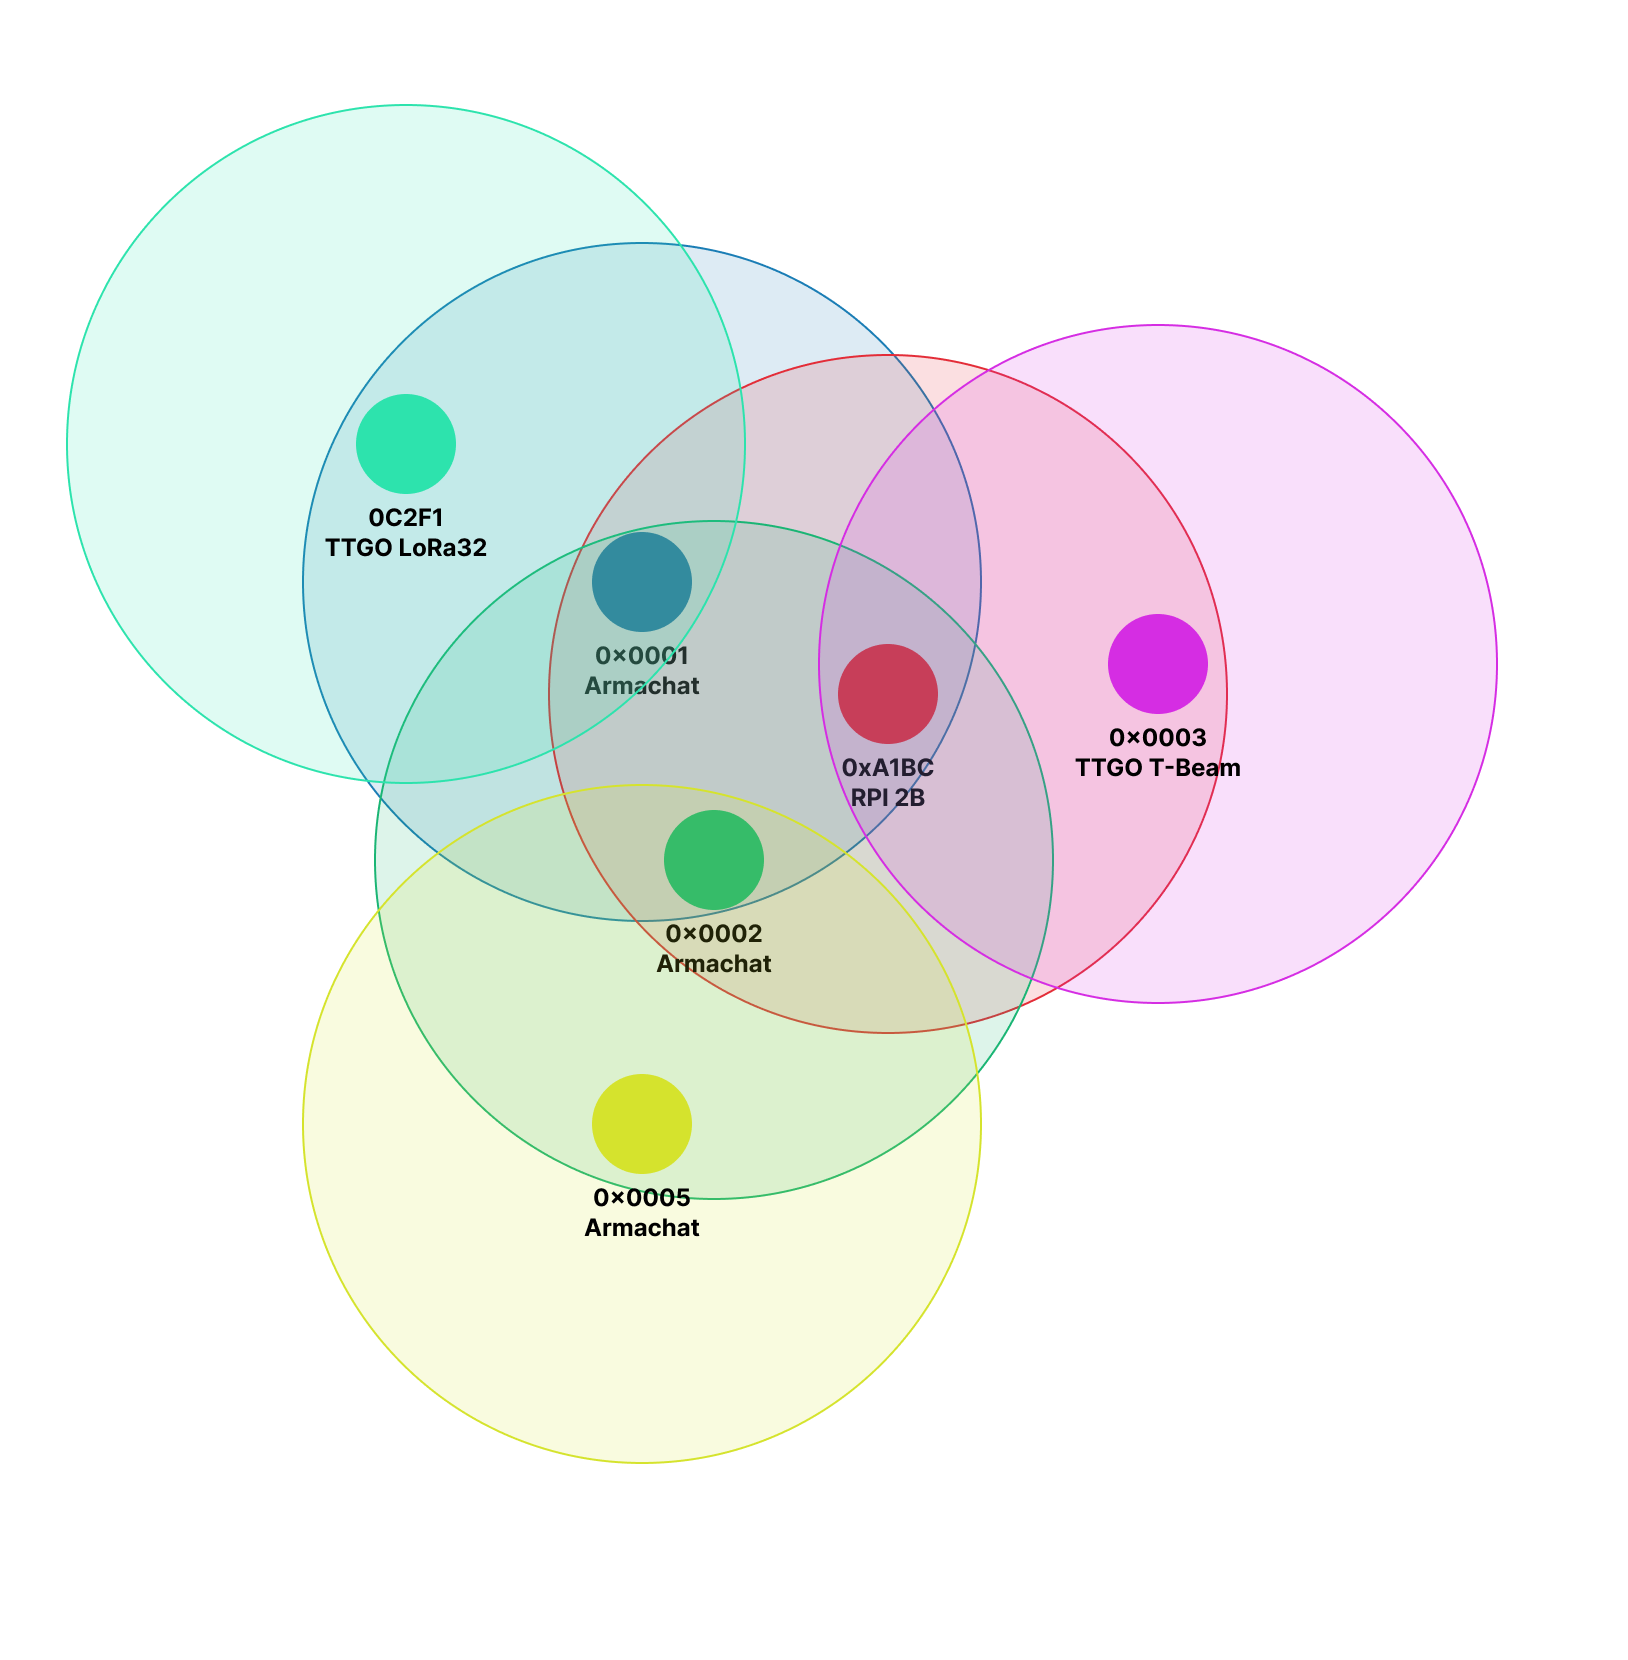
\includegraphics[width=0.8\textwidth]{Figures/topology.png}
  \caption{Rozmiestnenie zariadení použité pri testovaní}
  \label{fig:topology}
\end{figure}

- upravit nakres rozmiestnenia

- test ze to funguje, rozmiestnenie zariadeni, posielanie sprav, simulovanie sensorovych uzlov atd

- screenshoty z aplikacie

- test vykonnosti, packet loss, latency

- ttgo budu periodicky posielat senzor data na broadcast pripadne na 0x0005

- poslat traceroute z 0x0005 na 0x0001, ukazat vysledok

- na zariadeniach menit resend count z 1 na 5 a porovnat ako sa zmensuje packetloss s vyssim resend countom, spravit graf - packet loss vs resend count

\section{Problémy a limitácie}
Najväčším problémom, na ktorý sme narazili pri implementácii, bol spomínaný nedostatok pamäti na zariadeniach. Tento problém sa nám podarilo 
vyriešiť, ale nesie to so sebou istý kompromis v podobe obmedzeného počtu správ, ktoré môže jedno zariadenie u seba držať. Kvôli tomu, že na 
zariadení Armachat s WiFi modulom nám musel bežať webový server, bola pamäť zariadenia veľmi vyťažená. Limit na počet správ, ktoré môže zariadenie u seba držať, bol nastavený 
na 10 správ. 

Tento limit 10 správ, však v realite neznamenal až taký problém. Pokiaľ mal používateľ otvorené webové rozhranie tak sa správy ukladali aj na strane webovej aplikácie 
bežiacej v prehliadači používateľa. Ak došlo k dosiahnutiu maximálneho limitu správ tak sa z pamäte zariadenia odstránila najstaršia správa. V pamäti prehliadača na webovej aplikácii 
ale táto správa ostala. Takže používateľ bol schopný vidieť aj správy staršie ako posledných 10 správ.

Na zariadeniach Armachat bez WiFi modulu bolo možné vidieť len tu najnovšiu správu na displeji, takže limit 10 správ tu taktiež nebol problémom.

Veľkou limitáciou našej implementácie bolo, že CircuitPython nemá podporu pre externé prerušenia. Z toho dôvodu knižnica, ktorú sme použili na ovládanie zabudovaného LoRa modulu, 
nepracovala veľmi efektívne. Keď aktuálne LoRa modul prijímal nejaký paket, tak sa pozdržal cely zvyšok bežiaceho programu, až kým sa paket neprijal a neprečítal celý alebo kým nedošlo k vypršaniu 
časového limitu. Toto nam spomaľovalo beh programu zakaždým keď bol v sieti vysielaný nejaký paket.

Použitá knižnica na ovládanie LoRa modulu so sebou priniesla ešte dodatočnú limitáciu. Táto knižnica nesprávne pracovala s LoRa modulom a nebolo možné stabilne používať 
LoRa prenos pokiaľ bol nastavený rozprestierací faktor vyšší ako 9. Pri nastavení vyššieho rozprestieracieho faktoru sa spoľahlivosť prenosu dramaticky znížila. Pri 
našom testovaní sa nám nepodarilo úspešne doručiť ani jednu správu z desiatich pokusov pri použití najvyššieho rozprestieracieho faktoru. 
K tejto chybe existuje aj oficiálna chybová správa na GitHub stránke CircuitPython knižnice \cite{rfmIssue}.

Chybu v knižnici sme sa bezvýsledne snažili opraviť. Jedným z dôvodov, ktoré ku chybe prispievali bol nesprávne nastavený časový limit pre posielanie paketu. Knižnica odpočítavala časový limit dvoch sekúnd 
pri čítaní novo prijímaného paketu. Ak sa paket nestihol prečítať v tomto intervale tak sa čítanie prerušilo a prijatý paket sa zahodil. 
Avšak, keď sme si zobrali prípad paketu, ktorý mal veľkosť 100 bajtov a bol vysielaný s rozprestieracím faktorom 12, kódovacím pomerom 4/8, a šírkou pásma 125 kHz, zistili sme 
že čas potrebný na vyslanie tohto paketu sa blížil k 6 sekundám. Časový limit bol teda nedostačujúci na vysielanie paketov s vyššími rozprestieracími faktormi. Po 
zvýšení časového limitu v knižnici sme znovu otestovali spoľahlivosť prenosu. Tentokrát sa nam podarilo doručiť 2 správy z 10 pokusov. To avšak stále nebolo dostatočné a 
naznačovalo to, že problém bol ešte niekde inde. Ten sa nam už ale nepodarilo nájsť.

Zariadenie Raspberry Pi pico s WiFi modulom, bolo pomerné nové. CircuitPython knižnica pre podporu WiFi modulu je stále v beta verzií a ma veľa nedostatkov.
Neumožňovala prepnúť WiFi modul do režimu AP (Access Point) ak bol modul už predtým prepnutý do režimu station a rovnako nebolo možné prepnúť modul do režimu station ak bol 
už prepnutý do režimu AP. Jediný spôsob ako bolo možné WiFi modul úspešne prepnúť medzi režimami bolo tvrdé resetovanie zariadenia. 

Pôvodne sme mali v pláne implementovať štartovací proces zariadenia tak, že najskôr by sa zariadenie pokúsilo pripojiť k WiFi sieťam, ktoré malo uložené v zozname a ak sa mu nepodarilo 
pripojiť ku žiadnej z týchto sieti, tak vytvorilo svoju vlastnú WiFi sieť, na ktorú sa mohol používateľ pripojiť. Kvôli chybnému správaniu WiFi knižnice však tento prístup nebolo možné 
realizovať. V momente kedy sa snažil WiFi modul pripojiť na nejakú sieť zo zoznamu WiFi sieti, prepol sa do režimu station. Potom už nebolo možné modul prepnúť do režimu AP ak sa nepodarilo pripojiť 
k žiadnej zo sieti.

K WiFi knižnici sa viazal ešte jeden problém a to taký, že pokiaľ sa snažil používateľ pripojiť na webový server bežiaci na Armachat zariadení ihneď potom, ako sa zariadenie pripojilo na WiFi sieť, 
zariadenie sa dostalo do zamrznutého stavu a prestalo reagovať na čokoľvek. Na obnovenie funkcionality bol potrebný tvrdý reštart zariadenia. 
Tomuto problému sme sa snažili vyhýbať tak, že zariadenie zobrazovalo informáciu o spustenom web serveri až po určitom oneskorení a spoliehali sme na to, že používateľ 
sa bude pripájať na webový server až po zobrazení tejto informácie.

\chapter{Záver}
V tejto práci sa nam podarilo vytvoriť funkčný komunikačný protokol pre bezdrôtovú komunikáciu medzi zariadeniami v LoRa mesh sieti.
Funkcionalita protokolu bola otestovaná na rôznych zariadeniach kde bolo potvrdené, že protokol funguje správne. 

K obsluhe protokolu vzniklo webové rozhranie, na ktoré sa používateľ pripájal a mohol cez neho prijímať a odosielať správy, konfigurovať 
rôzne nastavenia, ktoré ovplyvňovali správanie protokolu, a spravovať zoznam kontaktov. Zoznam kontaktov slúžil na prekladanie 
hexadecimálnych adries zariadení na používateľom definované názvy.

Nami vytvorené riešenie je vhodné pre použitie v rôznych oblastiach, a ponúka oproti iným riešeniam isté výhody ako aj nevýhody.
Ak porovnáme naše riešenie voči niektorým spomínaným protokolom, ako napríklad LoRaBlink alebo Synchronous LoRa Mesh, 
tak náš protokol nie je závislý na žiadnych centrálnych uzloch, potrebných k riadeniu siete.

Naše riešenie by sa dalo prirovnať k projektu Meshtastic, ale oproti tomuto projektu ponúka naš protokol rôzne typy správ, ktoré umožňujú 
rozlične spracovávať správy zo senzorov a správy od používateľov. Okrem toho v našom protokole riešime aj slabinu projektu Meshtastic, ktorá 
sa prejavuje napríklad v situácií kedy by malo rozmiestnenie uzlov v sieti tvár písmena V.

Na obrázku \ref{fig:mestasticV} môžme vidieť takúto situáciu. Ak by sme z uzla číslo 0 chceli posielať správu do uzla číslo 4, nikdy by sa nám to nepodarilo.
A to z toho dôvodu, že vyslaná správa z uzlu 0 by bola prijatá uzlami 1 a 2, a keďže uzol 1 je od uzla 0 vzdialenejší ako uzol 2, bude mat horšiu hodnotu SNR.
Na základe horšej hodnoty SNR uzol 1 správu odvysiela skôr a správa sa ďalej bude šíriť už len v pravej vetve siete.

Na obrázku môžme vidieť rozmiestnenie uzlov a dosah ich signálu v simulátore Meshtasticator, patriaceho ku projektu Meshtastic. Taktiež môžme vidieť časový priebeh šírenia správy medzi uzlami. 
V tomto časovom priebehu su modrou farbou označené vysielania správy a zelenou prijatia správy.
\newpage
\begin{figure}[h!]
  \centering
  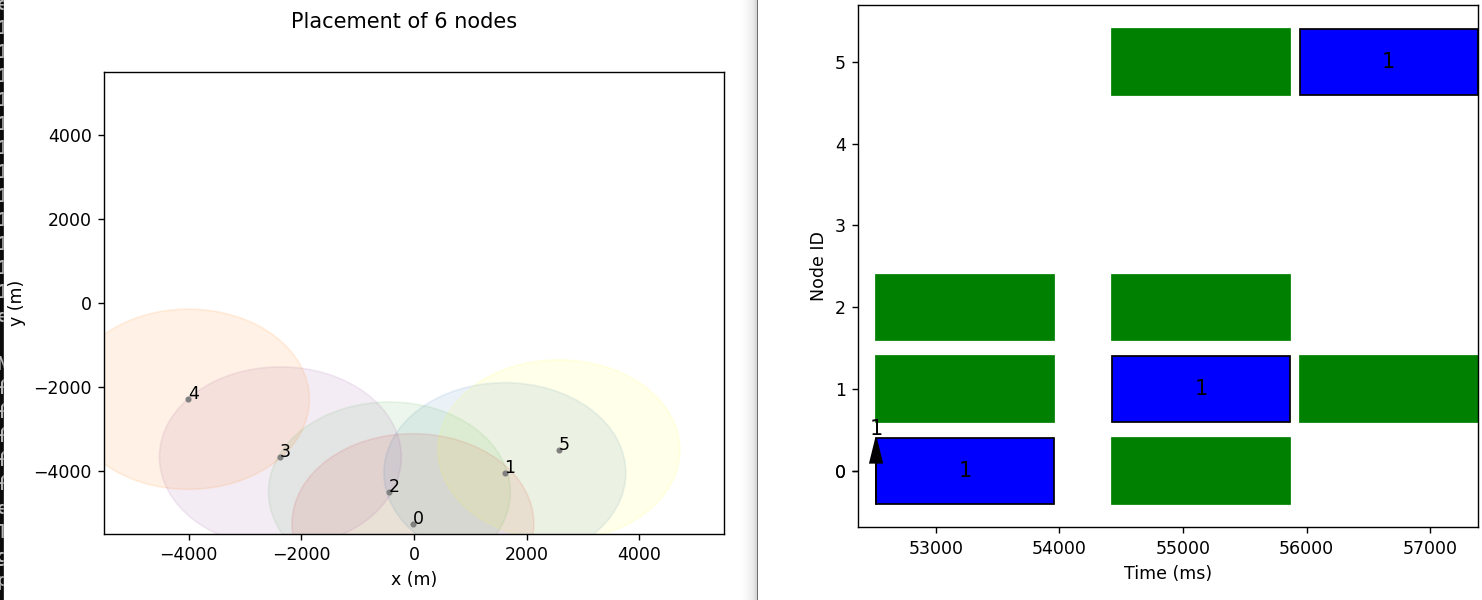
\includegraphics[width=0.8\textwidth]{Figures/meshtasticV.png}
  \caption{Meshtasticator simulátor}
  \label{fig:mestasticV}
\end{figure}

V našom riešení bolo pridané experimentálne nastavenie, ktoré po jeho zapnutí spôsobilo to, že poradie v ktorom sa správa odosielala z ďalších uzlov 
nebolo závislé na hodnote SNR ale bolo určovaná náhodne. Toto riešenie nebolo však úplne optimálne a vzhľadom na to, že poradie bolo určované 
náhodne,mohla nastať situácia, že náhodne vybraná trasa sa zhodovala s trasou vybranou 
na základe hodnôt SNR a správa sa teda tiež nedostala do cieľa. V tomto prípade bolo potrebné správu odoslať znovu. 
Tento problém by šlo optimálnejšie vyriešiť smerovacími tabuľkami, ktoré ale v našom protokole neboli použité.

Na obrázku \ref{fig:randomizePath} môžme vidieť časový priebeh šírenia správy medzi uzlami potom, čo sme upravili implementáciu simulátoru Meshtasticator tak, 
aby používal náhodnú trasu. Správa sa v tomto prípade už správne dostala z uzla 0 do uzla 4.

\begin{figure}[h!]
  \centering
  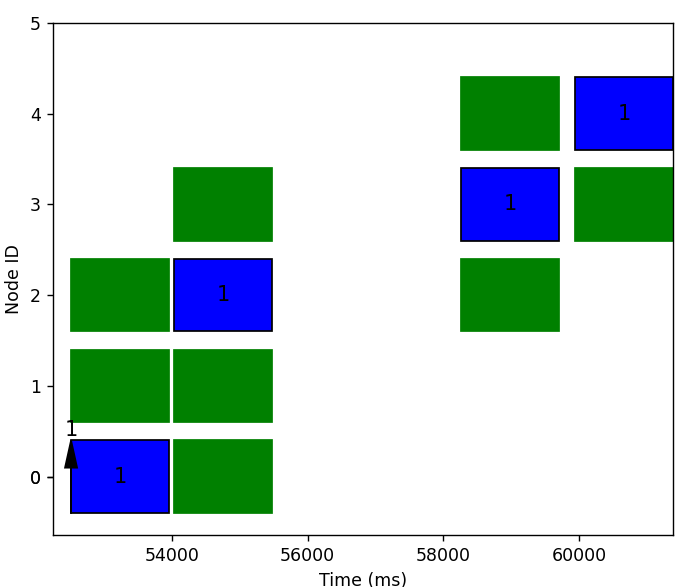
\includegraphics[width=0.4\textwidth]{Figures/randomizePath.png}
  \caption{Priebeh šírenia správy s náhodnou trasou}
  \label{fig:randomizePath}
\end{figure}

Náš protokol môže byť v budúcnosti rozšírený o ďalšie typy správ. Napríklad by bolo možné pridať nový typ správy určený pre binárne dáta, 
ktorá by sa mohla hodiť pri určitých aplikáciach. 
Taktiež by mohla byť funkcionalita rozšírená o možnosť rozdeľovať dlhšie správy na viacero menších správ, ktoré by sa potom posielali postupne.

% Seznam literatury
\printbibliography[title={Literatura}, heading=bibintoc]

% Prilohy
\appendix
\begin{figure}[]
  \centering
  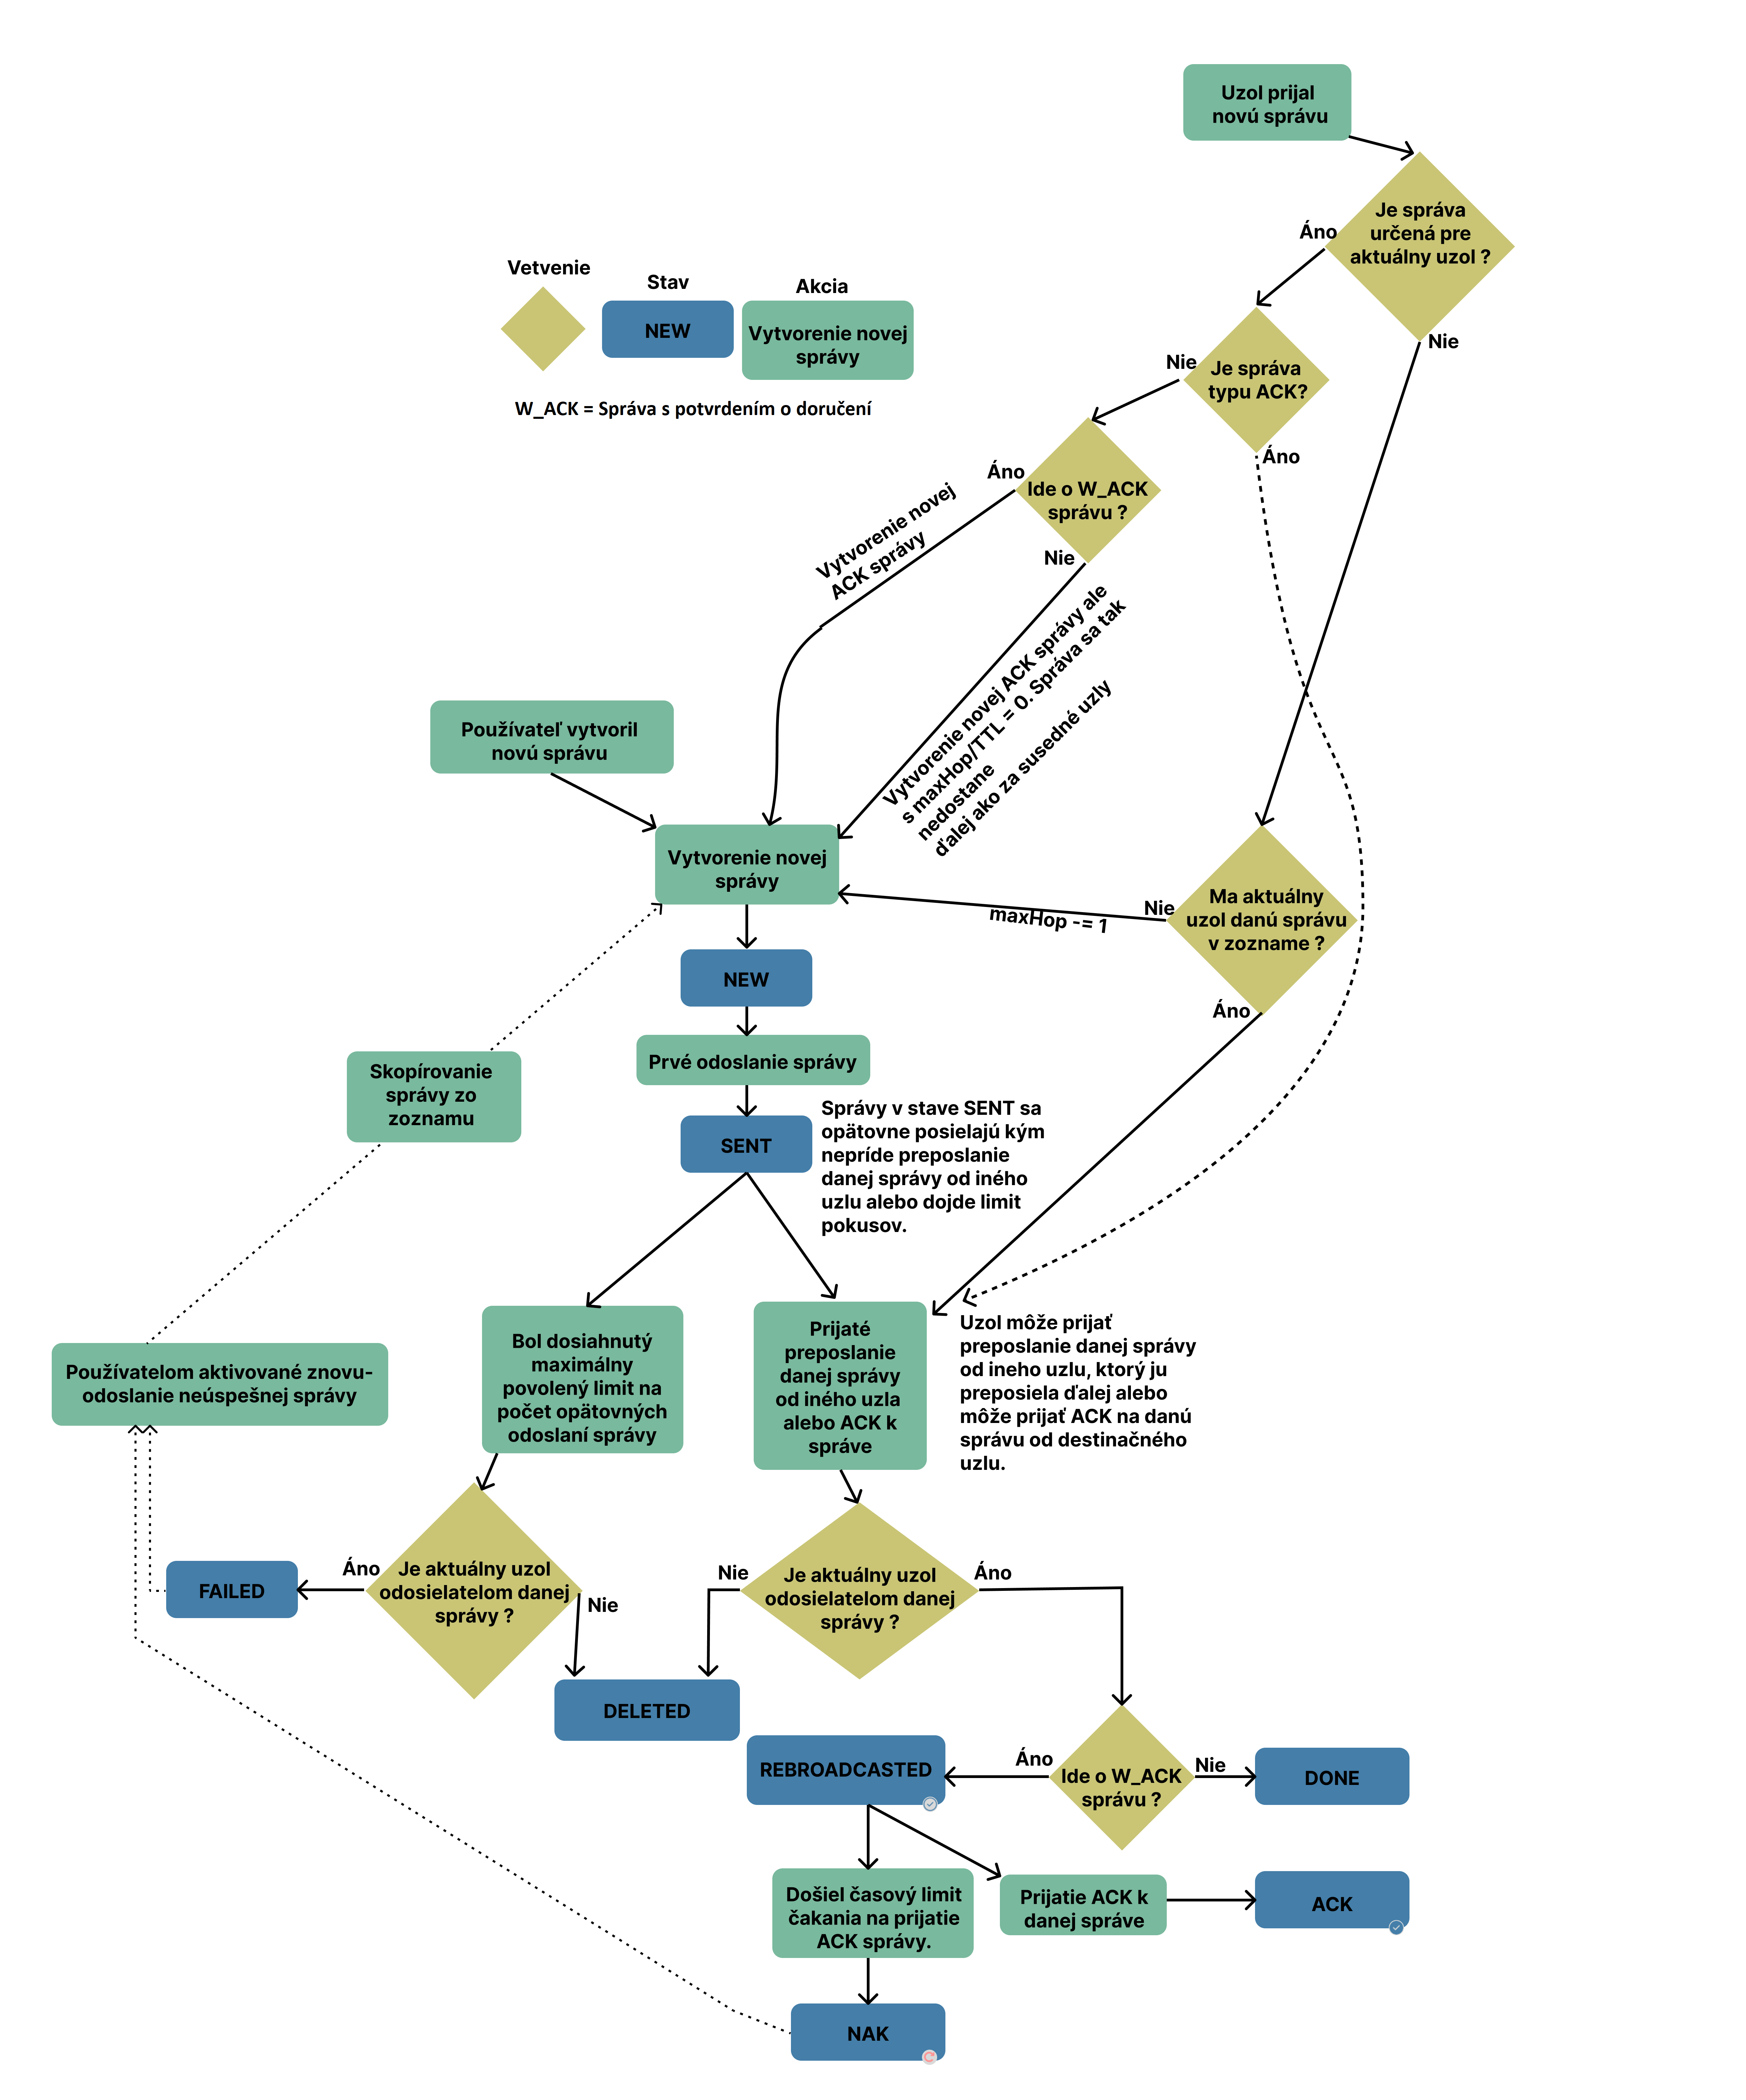
\includegraphics[width=1\textwidth]{Figures/state_flow_W.png}
  \caption{Zjednodušený stavový diagram}
  \label{fig:stateDiagram}
\end{figure}


\end{document}
